\documentclass{book}
\usepackage[a4paper,top=2.5cm,bottom=2.5cm,left=2.5cm,right=2.5cm]{geometry}
\usepackage{makeidx}
\usepackage{natbib}
\usepackage{graphicx}
\usepackage{multicol}
\usepackage{float}
\usepackage{listings}
\usepackage{color}
\usepackage{ifthen}
\usepackage[table]{xcolor}
\usepackage{textcomp}
\usepackage{alltt}
\usepackage{ifpdf}
\ifpdf
\usepackage[pdftex,
            pagebackref=true,
            colorlinks=true,
            linkcolor=blue,
            unicode
           ]{hyperref}
\else
\usepackage[ps2pdf,
            pagebackref=true,
            colorlinks=true,
            linkcolor=blue,
            unicode
           ]{hyperref}
\usepackage{pspicture}
\fi
\usepackage[utf8]{inputenc}
\usepackage{mathptmx}
\usepackage[scaled=.90]{helvet}
\usepackage{courier}
\usepackage{sectsty}
\usepackage{amssymb}
\usepackage[titles]{tocloft}
\usepackage{doxygen}
\lstset{language=C++,inputencoding=utf8,basicstyle=\footnotesize,breaklines=true,breakatwhitespace=true,tabsize=8,numbers=left }
\makeindex
\setcounter{tocdepth}{3}
\renewcommand{\footrulewidth}{0.4pt}
\renewcommand{\familydefault}{\sfdefault}
\hfuzz=15pt
\setlength{\emergencystretch}{15pt}
\hbadness=750
\tolerance=750
\begin{document}
\hypersetup{pageanchor=false,citecolor=blue}
\begin{titlepage}
\vspace*{7cm}
\begin{center}
{\Large Emma \\[1ex]\large 0.\-4 }\\
\vspace*{1cm}
{\large Generated by Doxygen 1.8.1.2}\\
\vspace*{0.5cm}
{\small Sun Dec 30 2012 13:02:49}\\
\end{center}
\end{titlepage}
\clearemptydoublepage
\pagenumbering{roman}
\tableofcontents
\clearemptydoublepage
\pagenumbering{arabic}
\hypersetup{pageanchor=true,citecolor=blue}
\chapter{File Index}
\section{File List}
Here is a list of all files with brief descriptions\-:\begin{DoxyCompactList}
\item\contentsline{section}{build/core/\hyperlink{colordoublearray_8cpp}{colordoublearray.\-cpp} }{\pageref{colordoublearray_8cpp}}{}
\item\contentsline{section}{build/core/\hyperlink{colorimage_8cpp}{colorimage.\-cpp} }{\pageref{colorimage_8cpp}}{}
\item\contentsline{section}{build/core/\hyperlink{comp__geometry_8cpp}{comp\-\_\-geometry.\-cpp} }{\pageref{comp__geometry_8cpp}}{}
\item\contentsline{section}{build/core/\hyperlink{doublearray_8cpp}{doublearray.\-cpp} }{\pageref{doublearray_8cpp}}{}
\item\contentsline{section}{build/core/\hyperlink{edge_8cpp}{edge.\-cpp} }{\pageref{edge_8cpp}}{}
\item\contentsline{section}{build/core/\hyperlink{ellipse_8cpp}{ellipse.\-cpp} }{\pageref{ellipse_8cpp}}{}
\item\contentsline{section}{build/core/\hyperlink{font_8cpp}{font.\-cpp} }{\pageref{font_8cpp}}{}
\item\contentsline{section}{build/core/\hyperlink{graph_8cpp}{graph.\-cpp} }{\pageref{graph_8cpp}}{}
\item\contentsline{section}{build/core/\hyperlink{graph__image_8cpp}{graph\-\_\-image.\-cpp} }{\pageref{graph__image_8cpp}}{}
\item\contentsline{section}{build/core/\hyperlink{int__images_8cpp}{int\-\_\-images.\-cpp} }{\pageref{int__images_8cpp}}{}
\item\contentsline{section}{build/core/\hyperlink{line_8cpp}{line.\-cpp} }{\pageref{line_8cpp}}{}
\item\contentsline{section}{build/core/\hyperlink{node_8cpp}{node.\-cpp} }{\pageref{node_8cpp}}{}
\item\contentsline{section}{build/core/\hyperlink{paint_8cpp}{paint.\-cpp} }{\pageref{paint_8cpp}}{}
\item\contentsline{section}{build/core/\hyperlink{plot_8cpp}{plot.\-cpp} }{\pageref{plot_8cpp}}{}
\item\contentsline{section}{build/core/\hyperlink{polygon_8cpp}{polygon.\-cpp} }{\pageref{polygon_8cpp}}{}
\item\contentsline{section}{build/core/\hyperlink{usr__misc_8cpp}{usr\-\_\-misc.\-cpp} }{\pageref{usr__misc_8cpp}}{}
\item\contentsline{section}{build/core/\hyperlink{vector3d_8cpp}{vector3d.\-cpp} }{\pageref{vector3d_8cpp}}{}
\item\contentsline{section}{build/io/\hyperlink{dcm_8cpp}{dcm.\-cpp} }{\pageref{dcm_8cpp}}{}
\item\contentsline{section}{build/io/\hyperlink{ema-fmt_8cpp}{ema-\/fmt.\-cpp} }{\pageref{ema-fmt_8cpp}}{}
\item\contentsline{section}{build/io/\hyperlink{graph__io_8cpp}{graph\-\_\-io.\-cpp} }{\pageref{graph__io_8cpp}}{}
\item\contentsline{section}{build/io/\hyperlink{image__io_8cpp}{image\-\_\-io.\-cpp} }{\pageref{image__io_8cpp}}{}
\item\contentsline{section}{build/io/\hyperlink{jpg_8cpp}{jpg.\-cpp} }{\pageref{jpg_8cpp}}{}
\item\contentsline{section}{build/io/\hyperlink{plot__io_8cpp}{plot\-\_\-io.\-cpp} }{\pageref{plot__io_8cpp}}{}
\item\contentsline{section}{build/io/\hyperlink{ppm_8cpp}{ppm.\-cpp} }{\pageref{ppm_8cpp}}{}
\end{DoxyCompactList}

\chapter{File Documentation}
\hypertarget{colordoublearray_8cpp}{\section{build/core/colordoublearray.cpp File Reference}
\label{colordoublearray_8cpp}\index{build/core/colordoublearray.\-cpp@{build/core/colordoublearray.\-cpp}}
}
{\ttfamily \#include \char`\"{}core/colordoublearray.\-h\char`\"{}}\\*
{\ttfamily \#include \char`\"{}core/int\-\_\-images.\-h\char`\"{}}\\*
Include dependency graph for colordoublearray.\-cpp\-:
\nopagebreak
\begin{figure}[H]
\begin{center}
\leavevmode
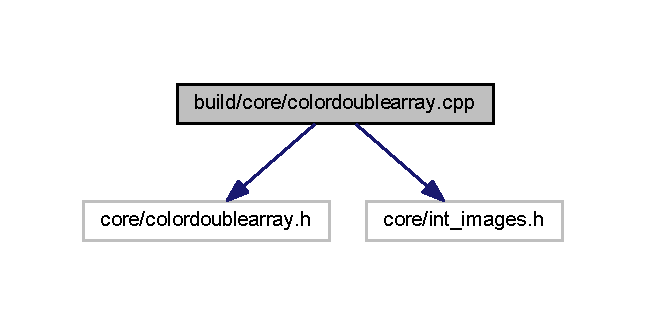
\includegraphics[width=310pt]{colordoublearray_8cpp__incl}
\end{center}
\end{figure}

\hypertarget{colorimage_8cpp}{\section{build/core/colorimage.cpp File Reference}
\label{colorimage_8cpp}\index{build/core/colorimage.\-cpp@{build/core/colorimage.\-cpp}}
}
{\ttfamily \#include \char`\"{}core/core.\-h\char`\"{}}\\*
{\ttfamily \#include \char`\"{}io/io.\-h\char`\"{}}\\*
{\ttfamily \#include $<$iostream$>$}\\*
Include dependency graph for colorimage.\-cpp\-:
\nopagebreak
\begin{figure}[H]
\begin{center}
\leavevmode
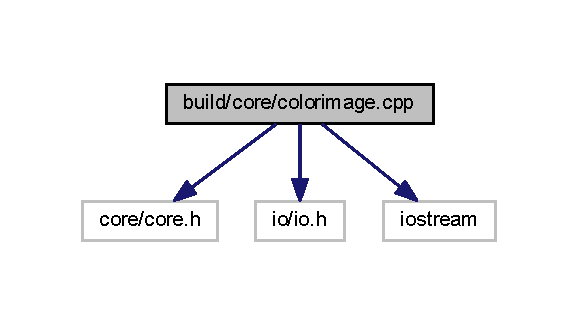
\includegraphics[width=278pt]{colorimage_8cpp__incl}
\end{center}
\end{figure}
\subsection*{Functions}
\begin{DoxyCompactItemize}
\item 
void \hyperlink{colorimage_8cpp_a045b42bc70d458788bc40b92a1ba5a18}{Transpose\-Color\-Array} (color $\ast$image, int N1, int N2, color $\ast$\&image\-T, int \&M1, int \&M2)
\end{DoxyCompactItemize}


\subsection{Function Documentation}
\hypertarget{colorimage_8cpp_a045b42bc70d458788bc40b92a1ba5a18}{\index{colorimage.\-cpp@{colorimage.\-cpp}!Transpose\-Color\-Array@{Transpose\-Color\-Array}}
\index{Transpose\-Color\-Array@{Transpose\-Color\-Array}!colorimage.cpp@{colorimage.\-cpp}}
\subsubsection[{Transpose\-Color\-Array}]{\setlength{\rightskip}{0pt plus 5cm}void Transpose\-Color\-Array (
\begin{DoxyParamCaption}
\item[{color $\ast$}]{image, }
\item[{int}]{N1, }
\item[{int}]{N2, }
\item[{color $\ast$\&}]{image\-T, }
\item[{int \&}]{M1, }
\item[{int \&}]{M2}
\end{DoxyParamCaption}
)}}\label{colorimage_8cpp_a045b42bc70d458788bc40b92a1ba5a18}


Definition at line 7 of file colorimage.\-cpp.


\hypertarget{comp__geometry_8cpp}{\section{build/core/comp\-\_\-geometry.cpp File Reference}
\label{comp__geometry_8cpp}\index{build/core/comp\-\_\-geometry.\-cpp@{build/core/comp\-\_\-geometry.\-cpp}}
}
{\ttfamily \#include $<$iostream$>$}\\*
{\ttfamily \#include $<$math.\-h$>$}\\*
{\ttfamily \#include $<$fstream$>$}\\*
{\ttfamily \#include $<$queue$>$}\\*
{\ttfamily \#include \char`\"{}core/common.\-h\char`\"{}}\\*
{\ttfamily \#include \char`\"{}core/comp\-\_\-geometry.\-h\char`\"{}}\\*
Include dependency graph for comp\-\_\-geometry.\-cpp\-:
\nopagebreak
\begin{figure}[H]
\begin{center}
\leavevmode
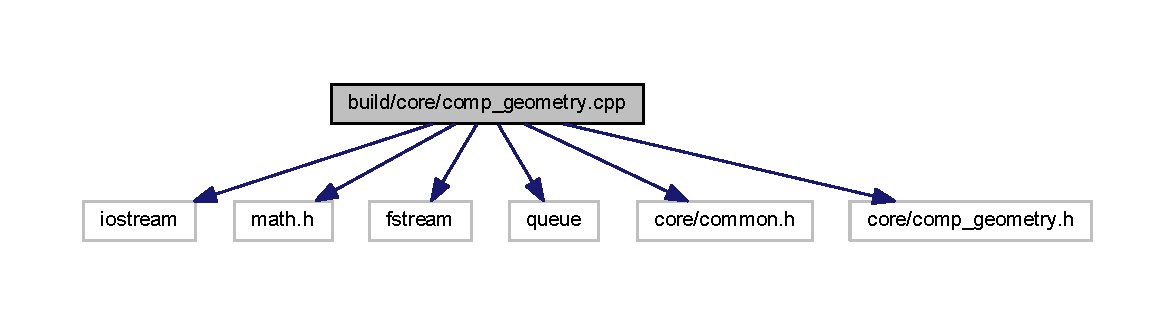
\includegraphics[width=350pt]{comp__geometry_8cpp__incl}
\end{center}
\end{figure}
\subsection*{Functions}
\begin{DoxyCompactItemize}
\item 
point \hyperlink{comp__geometry_8cpp_af347554b700856d257b5d3b6947778dd}{Polygon\-Centroid} (point $\ast$p, int np, double $\ast$area)
\item 
bool \hyperlink{comp__geometry_8cpp_a0ef1b95f8118540e26d99ae423b9b385}{Segment\-Intersect} (double Ax, double Ay, double Bx, double By, double Cx, double Cy, double Dx, double Dy, double \&X, double \&Y)
\item 
int \hyperlink{comp__geometry_8cpp_aac9e1c9ec2e6dd9d8ac0d147d72f2102}{Point\-In\-Polygon\-Test} (point $\ast$p, int N, double x, double y)
\item 
bool \hyperlink{comp__geometry_8cpp_a249e4aef00b1f29f718d33328e86edfb}{Poly\-Poly\-Intersect} (point $\ast$p, int np, point $\ast$q, int nq)
\item 
void \hyperlink{comp__geometry_8cpp_a7da8af9c400ec6d4dc1158c289ce579c}{Read\-Polygon} (char $\ast$poly\-\_\-file, polygon $\ast$poly)
\item 
void \hyperlink{comp__geometry_8cpp_a4028b729f373ea5ad22cfba68ac66df5}{Save\-Polygon} (polygon $\ast$poly, char $\ast$poly\-\_\-file)
\end{DoxyCompactItemize}


\subsection{Function Documentation}
\hypertarget{comp__geometry_8cpp_aac9e1c9ec2e6dd9d8ac0d147d72f2102}{\index{comp\-\_\-geometry.\-cpp@{comp\-\_\-geometry.\-cpp}!Point\-In\-Polygon\-Test@{Point\-In\-Polygon\-Test}}
\index{Point\-In\-Polygon\-Test@{Point\-In\-Polygon\-Test}!comp_geometry.cpp@{comp\-\_\-geometry.\-cpp}}
\subsubsection[{Point\-In\-Polygon\-Test}]{\setlength{\rightskip}{0pt plus 5cm}int Point\-In\-Polygon\-Test (
\begin{DoxyParamCaption}
\item[{point $\ast$}]{p, }
\item[{int}]{N, }
\item[{double}]{x, }
\item[{double}]{y}
\end{DoxyParamCaption}
)}}\label{comp__geometry_8cpp_aac9e1c9ec2e6dd9d8ac0d147d72f2102}


Definition at line 100 of file comp\-\_\-geometry.\-cpp.

\hypertarget{comp__geometry_8cpp_af347554b700856d257b5d3b6947778dd}{\index{comp\-\_\-geometry.\-cpp@{comp\-\_\-geometry.\-cpp}!Polygon\-Centroid@{Polygon\-Centroid}}
\index{Polygon\-Centroid@{Polygon\-Centroid}!comp_geometry.cpp@{comp\-\_\-geometry.\-cpp}}
\subsubsection[{Polygon\-Centroid}]{\setlength{\rightskip}{0pt plus 5cm}point Polygon\-Centroid (
\begin{DoxyParamCaption}
\item[{point $\ast$}]{p, }
\item[{int}]{np, }
\item[{double $\ast$}]{area}
\end{DoxyParamCaption}
)}}\label{comp__geometry_8cpp_af347554b700856d257b5d3b6947778dd}


Definition at line 11 of file comp\-\_\-geometry.\-cpp.

\hypertarget{comp__geometry_8cpp_a249e4aef00b1f29f718d33328e86edfb}{\index{comp\-\_\-geometry.\-cpp@{comp\-\_\-geometry.\-cpp}!Poly\-Poly\-Intersect@{Poly\-Poly\-Intersect}}
\index{Poly\-Poly\-Intersect@{Poly\-Poly\-Intersect}!comp_geometry.cpp@{comp\-\_\-geometry.\-cpp}}
\subsubsection[{Poly\-Poly\-Intersect}]{\setlength{\rightskip}{0pt plus 5cm}bool Poly\-Poly\-Intersect (
\begin{DoxyParamCaption}
\item[{point $\ast$}]{p, }
\item[{int}]{np, }
\item[{point $\ast$}]{q, }
\item[{int}]{nq}
\end{DoxyParamCaption}
)}}\label{comp__geometry_8cpp_a249e4aef00b1f29f718d33328e86edfb}


Definition at line 116 of file comp\-\_\-geometry.\-cpp.



Here is the call graph for this function\-:
\nopagebreak
\begin{figure}[H]
\begin{center}
\leavevmode
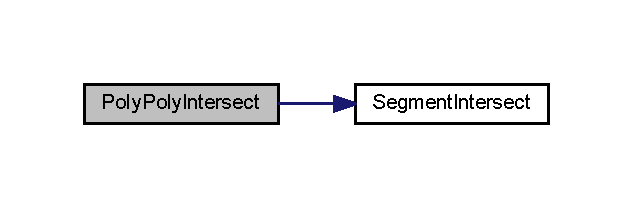
\includegraphics[width=304pt]{comp__geometry_8cpp_a249e4aef00b1f29f718d33328e86edfb_cgraph}
\end{center}
\end{figure}


\hypertarget{comp__geometry_8cpp_a7da8af9c400ec6d4dc1158c289ce579c}{\index{comp\-\_\-geometry.\-cpp@{comp\-\_\-geometry.\-cpp}!Read\-Polygon@{Read\-Polygon}}
\index{Read\-Polygon@{Read\-Polygon}!comp_geometry.cpp@{comp\-\_\-geometry.\-cpp}}
\subsubsection[{Read\-Polygon}]{\setlength{\rightskip}{0pt plus 5cm}void Read\-Polygon (
\begin{DoxyParamCaption}
\item[{char $\ast$}]{poly\-\_\-file, }
\item[{polygon $\ast$}]{poly}
\end{DoxyParamCaption}
)}}\label{comp__geometry_8cpp_a7da8af9c400ec6d4dc1158c289ce579c}


Definition at line 135 of file comp\-\_\-geometry.\-cpp.



Here is the call graph for this function\-:
\nopagebreak
\begin{figure}[H]
\begin{center}
\leavevmode
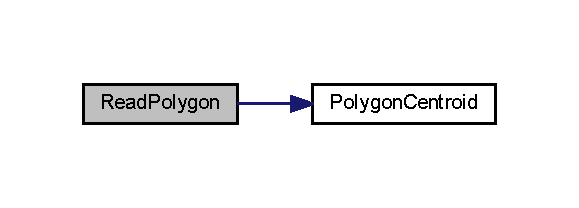
\includegraphics[width=278pt]{comp__geometry_8cpp_a7da8af9c400ec6d4dc1158c289ce579c_cgraph}
\end{center}
\end{figure}


\hypertarget{comp__geometry_8cpp_a4028b729f373ea5ad22cfba68ac66df5}{\index{comp\-\_\-geometry.\-cpp@{comp\-\_\-geometry.\-cpp}!Save\-Polygon@{Save\-Polygon}}
\index{Save\-Polygon@{Save\-Polygon}!comp_geometry.cpp@{comp\-\_\-geometry.\-cpp}}
\subsubsection[{Save\-Polygon}]{\setlength{\rightskip}{0pt plus 5cm}void Save\-Polygon (
\begin{DoxyParamCaption}
\item[{polygon $\ast$}]{poly, }
\item[{char $\ast$}]{poly\-\_\-file}
\end{DoxyParamCaption}
)}}\label{comp__geometry_8cpp_a4028b729f373ea5ad22cfba68ac66df5}


Definition at line 164 of file comp\-\_\-geometry.\-cpp.

\hypertarget{comp__geometry_8cpp_a0ef1b95f8118540e26d99ae423b9b385}{\index{comp\-\_\-geometry.\-cpp@{comp\-\_\-geometry.\-cpp}!Segment\-Intersect@{Segment\-Intersect}}
\index{Segment\-Intersect@{Segment\-Intersect}!comp_geometry.cpp@{comp\-\_\-geometry.\-cpp}}
\subsubsection[{Segment\-Intersect}]{\setlength{\rightskip}{0pt plus 5cm}bool Segment\-Intersect (
\begin{DoxyParamCaption}
\item[{double}]{Ax, }
\item[{double}]{Ay, }
\item[{double}]{Bx, }
\item[{double}]{By, }
\item[{double}]{Cx, }
\item[{double}]{Cy, }
\item[{double}]{Dx, }
\item[{double}]{Dy, }
\item[{double \&}]{X, }
\item[{double \&}]{Y}
\end{DoxyParamCaption}
)}}\label{comp__geometry_8cpp_a0ef1b95f8118540e26d99ae423b9b385}


Definition at line 49 of file comp\-\_\-geometry.\-cpp.


\hypertarget{doublearray_8cpp}{\section{build/core/doublearray.cpp File Reference}
\label{doublearray_8cpp}\index{build/core/doublearray.\-cpp@{build/core/doublearray.\-cpp}}
}
{\ttfamily \#include \char`\"{}core/core.\-h\char`\"{}}\\*
{\ttfamily \#include $<$math.\-h$>$}\\*
{\ttfamily \#include $<$stdio.\-h$>$}\\*
{\ttfamily \#include $<$iostream$>$}\\*
Include dependency graph for doublearray.\-cpp\-:
\nopagebreak
\begin{figure}[H]
\begin{center}
\leavevmode
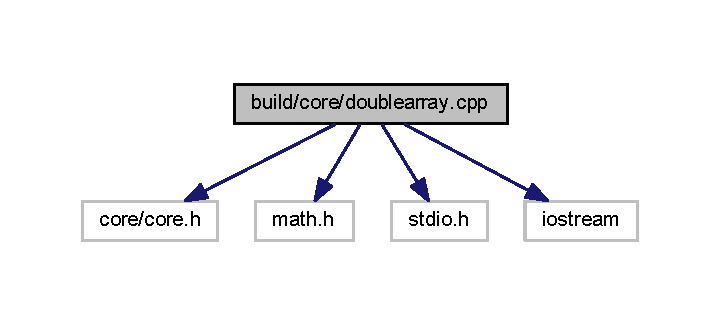
\includegraphics[width=346pt]{doublearray_8cpp__incl}
\end{center}
\end{figure}
\subsection*{Functions}
\begin{DoxyCompactItemize}
\item 
void \hyperlink{doublearray_8cpp_a0fe1cc9dcb110c5e9936c113d23a5ee0}{Paint\-By\-Numbers\-Double\-Array} (double $\ast$$\ast$arrs, int M1, int M2, int $\ast$labels, int L1, int L2, double $\ast$\&arr, int \&N1, int \&N2)
\item 
void \hyperlink{doublearray_8cpp_ae4e3b80458efff3f8e6756b8b9cc27a3}{Edges\-Laplacian\-Double\-Array} (double $\ast$arr, double $\ast$\&arr\-Out, int N1, int N2)
\item 
void \hyperlink{doublearray_8cpp_af3f1295a7e4a75c43907db64e40c2400}{Edges\-Sobel\-Double\-Array} (double $\ast$arr, double $\ast$\&arr\-Out, int N1, int N2)
\item 
void \hyperlink{doublearray_8cpp_ac683b719f8ce63556a6bcc0f7f306acd}{Stretch\-Double\-Array} (double $\ast$\&arr, int N1, int N2)
\item 
void \hyperlink{doublearray_8cpp_ac53c7e23c21938b1554e363ea46fb9ef}{Divide\-Double\-Arrays} (double $\ast$image1, double $\ast$image2, double $\ast$\&image\-Out, int N1, int N2)
\item 
void \hyperlink{doublearray_8cpp_ac30d94a9a4077fa308d6489ef0ef01a1}{Threshold\-Double\-Array} (double $\ast$\&arr, double threshold\-Low, double threshold\-High, int N1, int N2)
\item 
void \hyperlink{doublearray_8cpp_a05115ec8293000a3163007bcf88ee956}{Minimum\-Maximum\-Of\-Array} (double $\ast$arr, int N1, int N2, double \&min1, double \&max1)
\item 
void \hyperlink{doublearray_8cpp_a6641c67e5167774ccfcd0beb47a4df1b}{Log\-Double\-Array} (double $\ast$arr, int N1, int N2)
\item 
void \hyperlink{doublearray_8cpp_acad3a906d768ee20770f375fbf70a952}{Scale\-Double\-Array} (double $\ast$\&arr, double scalar, int N1, int N2)
\item 
void \hyperlink{doublearray_8cpp_acacf2689331cb439d1bebef68a1f8552}{Output\-Double\-Array\-To\-File} (char $\ast$filename, double $\ast$arr, int N1, int N2)
\item 
void \hyperlink{doublearray_8cpp_af5ae02f38013ee530b629f5e2cbb4093}{Copy\-Double\-To\-Double\-Array} (double $\ast$arr, double $\ast$\&arr\-Out, int N1, int N2)
\item 
void \hyperlink{doublearray_8cpp_a73c1563b450e254d24e80b7292b54ea5}{Draw\-Line\-In\-Double\-Array\-\_\-\-D\-D\-A} (double $\ast$\&arr, int N1, int N2, double x1, double y1, double x2, double y2, double val)
\item 
void \hyperlink{doublearray_8cpp_aa1bd64811b94064d93db7b17b0b3daca}{Polygon\-Double\-Array} (double $\ast$arr, int N1, int N2, point\-Double $\ast$p, int N, double x, double y, double W, double H, double val)
\item 
void \hyperlink{doublearray_8cpp_a1dc3c3f85d1bb420090295c8cd7b2499}{Rotate\-Angle\-Double\-Array} (double $\ast$arr, double $\ast$\&arr\-Out, int N1, int N2, double Radians)
\item 
void \hyperlink{doublearray_8cpp_a15e257b0d36560b30c262874f54f4a8b}{Rotate\-Right\-Double\-Array} (double $\ast$arr, int N1, int N2, double $\ast$\&arr\-Out, int \&M1, int \&M2)
\item 
void \hyperlink{doublearray_8cpp_a7c28b9f7097580074d8a9107f93fbd46}{Rotate\-Left\-Double\-Array} (double $\ast$arr, int N1, int N2, double $\ast$\&arr\-Out, int \&M1, int \&M2)
\item 
void \hyperlink{doublearray_8cpp_a4ef5c8e4ce7b4089ed2b89dc1d9c4e60}{Draw\-Line\-In\-Double\-Array} (double $\ast$\&arr, int N1, int N2, double x1, double y1, double x2, double y2, double val)
\item 
void \hyperlink{doublearray_8cpp_a500bba1190ba419fdab522f1dc7ab0aa}{Draw\-Line\-In\-Double\-Array\-\_\-\-N} (double $\ast$\&arr, int N1, int N2, double x1, double y1, double x2, double y2, double val, int N)
\item 
void \hyperlink{doublearray_8cpp_af26847f3b9f9980d624eb02b8c1212d7}{Draw\-Line\-In\-Double\-Array\-\_\-\-Bresenham\-\_\-\-N} (double $\ast$\&arr, int N1, int N2, double x1, double y1, double x2, double y2, double val, int N)
\item 
void \hyperlink{doublearray_8cpp_aefad9e5bcdd81f7f4e4cf0d694fc9dfb}{Draw\-Line\-In\-Double\-Array\-\_\-\-Bresenham} (double $\ast$\&arr, int N1, int N2, double x1, double y1, double x2, double y2, double val)
\item 
void \hyperlink{doublearray_8cpp_a452d0462be3b1c1229d65dd45c54298c}{Draw\-Line\-In\-Double\-Array\-\_\-\-D\-D\-A\-\_\-\-N} (double $\ast$\&arr, int N1, int N2, double x1, double y1, double x2, double y2, double val, int N)
\item 
void \hyperlink{doublearray_8cpp_acd3ed79a855f210de95c5202c5942756}{Draw\-Line\-In\-Double\-Array\-\_\-\-D\-D\-A\-\_\-\-N\-\_\-\-Helper} (double $\ast$\&arr, int N1, int N2, double x1, double y1, double x2, double y2, double val, int dn)
\item 
void \hyperlink{doublearray_8cpp_a52a21b223027d4451e19d0ba82ee7824}{Convolve\-Double\-Arrays} (double $\ast$arr1, double $\ast$arr2, double $\ast$\&arr3, int N1, int N2, int M1, int M2)
\item 
void \hyperlink{doublearray_8cpp_a511dff95c8f666b13a0d680d5c69c428}{Flip\-Vertical\-Double\-Array} (double $\ast$arr, double $\ast$arr\-Out, int N1, int N2)
\item 
void \hyperlink{doublearray_8cpp_ab3052e47549b941dce4a630a7fb3c7c1}{Flip\-Horizontal\-Double\-Array} (double $\ast$arr, double $\ast$arr\-Out, int N1, int N2)
\item 
void \hyperlink{doublearray_8cpp_a97bb928aff6f1afad8b0dfa3d703535e}{Locate\-Min\-Max\-Double\-Array} (double $\ast$arr, int N1, int N2, double \&min1, double \&max1, int \&mini, int \&minj, int \&maxi, int \&maxj)
\item 
void \hyperlink{doublearray_8cpp_ae050ddd846c56f992b5c5175ed449ad8}{Paste\-With\-Mask\-Double\-Array} (double $\ast$\&arr1, double $\ast$arr2, double $\ast$mask2, double x, double y, int N1, int N2, int M1, int M2)
\item 
void \hyperlink{doublearray_8cpp_a68d66dd58f1de9c0778ff6f80ab10dea}{Clip\-Double\-Array\-Using\-Z\-Score} (double $\ast$\&arr, double mean, double sigma, double Z\-Score, int N1, int N2)
\item 
void \hyperlink{doublearray_8cpp_aca71249ab74852cdecb47ad9b9e43f0f}{Statistics\-Of\-Double\-Array} (double $\ast$arr, double \&mean, double \&sigma, int N1, int N2)
\item 
void \hyperlink{doublearray_8cpp_a7cd45c83e7d79a0ed7529a02e8c2831a}{Subtract\-Scalar\-From\-Double\-Array} (double $\ast$\&arr, double scalar, int N1, int N2)
\item 
void \hyperlink{doublearray_8cpp_aa61d08caadf680da67f5fd233fb44ecc}{Subtract\-Double\-Arrays} (double $\ast$arr1, double $\ast$arr2, double $\ast$\&arr\-Out, int N1, int N2)
\item 
void \hyperlink{doublearray_8cpp_a94a0f3e08aecc9874677682fd5c982d2}{Close\-Double\-Array2} (double $\ast$arr, double $\ast$\&arr\-Out, int N1, int N2)
\item 
void \hyperlink{doublearray_8cpp_afcfc024419938e3553b330a315bc92cf}{Open\-Double\-Array2} (double $\ast$arr, double $\ast$\&arr\-Out, int N1, int N2)
\item 
void \hyperlink{doublearray_8cpp_a270594add95139649fdc8e84caa67169}{Transpose\-Double\-Array} (double $\ast$arr, int N1, int N2, double $\ast$\&arr\-Out, int \&M1, int \&M2)
\item 
void \hyperlink{doublearray_8cpp_a086d2dccfe8cbef8a954881b6aae65c1}{Multiply\-Double\-Arrays} (double $\ast$arr1, double $\ast$arr2, double $\ast$\&arr\-Out, int N1, int N2, int N3)
\item 
void \hyperlink{doublearray_8cpp_a05c67876c6eb936bce9e5d33ca8401ca}{Close\-Double\-Array} (double $\ast$\&arr, int N1, int N2)
\item 
void \hyperlink{doublearray_8cpp_a8199fd9d2030481ef8a987aef3b79634}{Open\-Double\-Array} (double $\ast$\&arr, int N1, int N2)
\item 
void \hyperlink{doublearray_8cpp_a04e473474ee3f5ab5d0c2591e1ee83d7}{Display\-Double\-Array} (double $\ast$arr, int R\-O\-W, int C\-O\-L)
\item 
void \hyperlink{doublearray_8cpp_accc37377f8bbbac93ac42802726741b5}{Dilate\-Double\-Array} (double $\ast$\&arr, int N1, int N2)
\item 
void \hyperlink{doublearray_8cpp_ac025547a3c77be19835c883ce233d902}{Erode\-Double\-Array} (double $\ast$\&arr, int N1, int N2)
\item 
void \hyperlink{doublearray_8cpp_aa26e1056a74ba31a3081a7b63a72ae0f}{Center\-Double\-Array} (double $\ast$\&arr, int N1, int N2)
\item 
void \hyperlink{doublearray_8cpp_aa074caff8bf0bb069a3f35a7f6bb4572}{Scale\-Size\-Double\-Array} (double $\ast$arr, double $\ast$\&arr\-Out, double sx, double sy, int N1, int N2, int \&M1, int \&M2)
\item 
void \hyperlink{doublearray_8cpp_ad38de193265b9dee386ec39996cf8612}{Translate\-Double\-Array} (double $\ast$arr, double $\ast$\&arr\-Out, double tx, double ty, int N1, int N2)
\item 
void \hyperlink{doublearray_8cpp_a4ae6098a7845fac0944ad664cb1abf79}{Dilate\-Double\-Array2} (double $\ast$arr, double $\ast$\&arr\-Out, int N1, int N2)
\item 
void \hyperlink{doublearray_8cpp_a05656fb702a00b8149dfa78bfae2582c}{Erode\-Double\-Array2} (double $\ast$arr, double $\ast$\&arr\-Out, int N1, int N2)
\item 
void \hyperlink{doublearray_8cpp_a18bd2f80b4e24d8ba98fd4ad0601b967}{Zero\-Double\-Array} (double $\ast$\&arr, int N1, int N2)
\item 
void \hyperlink{doublearray_8cpp_a85218774a5ad8746e40d11332f667e6a}{Add\-Double\-Array2} (double $\ast$\&arr1, double $\ast$arr2, double x, double y, int N1, int N2, int M1, int M2)
\item 
void \hyperlink{doublearray_8cpp_a3ae59dd7b331d1958c77d6c81391f491}{Subtract\-Double\-Array2} (double $\ast$\&arr1, double $\ast$arr2, double x, double y, int N1, int N2, int M1, int M2)
\item 
void \hyperlink{doublearray_8cpp_abff31a105bf6a91afd998deacdbf4d44}{Paste\-Double\-Array} (double $\ast$\&arr1, double $\ast$arr2, double x, double y, int N1, int N2, int M1, int M2)
\item 
void \hyperlink{doublearray_8cpp_a0901a62db5e9b8f00bb8d74b2f663061}{Extend\-Double\-Array} (double $\ast$arr, double $\ast$\&arr\-Out, double x, double y, int N1, int N2, int M1, int M2)
\item 
void \hyperlink{doublearray_8cpp_a5fa9442cc8a6b938abb47f05e4ab9b85}{Add\-Double\-Array} (double $\ast$arr1, double $\ast$arr2, double $\ast$\&arr\-Out, int N1, int N2)
\item 
void \hyperlink{doublearray_8cpp_a0598de03486bc65c7ae493e7dbcd9382}{Abs\-Double\-Array} (double $\ast$\&arr, int N1, int N2)
\end{DoxyCompactItemize}


\subsection{Function Documentation}
\hypertarget{doublearray_8cpp_a0598de03486bc65c7ae493e7dbcd9382}{\index{doublearray.\-cpp@{doublearray.\-cpp}!Abs\-Double\-Array@{Abs\-Double\-Array}}
\index{Abs\-Double\-Array@{Abs\-Double\-Array}!doublearray.cpp@{doublearray.\-cpp}}
\subsubsection[{Abs\-Double\-Array}]{\setlength{\rightskip}{0pt plus 5cm}void Abs\-Double\-Array (
\begin{DoxyParamCaption}
\item[{double $\ast$\&}]{arr, }
\item[{int}]{N1, }
\item[{int}]{N2}
\end{DoxyParamCaption}
)}}\label{doublearray_8cpp_a0598de03486bc65c7ae493e7dbcd9382}


Definition at line 930 of file doublearray.\-cpp.

\hypertarget{doublearray_8cpp_a5fa9442cc8a6b938abb47f05e4ab9b85}{\index{doublearray.\-cpp@{doublearray.\-cpp}!Add\-Double\-Array@{Add\-Double\-Array}}
\index{Add\-Double\-Array@{Add\-Double\-Array}!doublearray.cpp@{doublearray.\-cpp}}
\subsubsection[{Add\-Double\-Array}]{\setlength{\rightskip}{0pt plus 5cm}void Add\-Double\-Array (
\begin{DoxyParamCaption}
\item[{double $\ast$}]{arr1, }
\item[{double $\ast$}]{arr2, }
\item[{double $\ast$\&}]{arr\-Out, }
\item[{int}]{N1, }
\item[{int}]{N2}
\end{DoxyParamCaption}
)}}\label{doublearray_8cpp_a5fa9442cc8a6b938abb47f05e4ab9b85}


Definition at line 922 of file doublearray.\-cpp.

\hypertarget{doublearray_8cpp_a85218774a5ad8746e40d11332f667e6a}{\index{doublearray.\-cpp@{doublearray.\-cpp}!Add\-Double\-Array2@{Add\-Double\-Array2}}
\index{Add\-Double\-Array2@{Add\-Double\-Array2}!doublearray.cpp@{doublearray.\-cpp}}
\subsubsection[{Add\-Double\-Array2}]{\setlength{\rightskip}{0pt plus 5cm}void Add\-Double\-Array2 (
\begin{DoxyParamCaption}
\item[{double $\ast$\&}]{arr1, }
\item[{double $\ast$}]{arr2, }
\item[{double}]{x, }
\item[{double}]{y, }
\item[{int}]{N1, }
\item[{int}]{N2, }
\item[{int}]{M1, }
\item[{int}]{M2}
\end{DoxyParamCaption}
)}}\label{doublearray_8cpp_a85218774a5ad8746e40d11332f667e6a}


Definition at line 863 of file doublearray.\-cpp.



Here is the call graph for this function\-:
\nopagebreak
\begin{figure}[H]
\begin{center}
\leavevmode
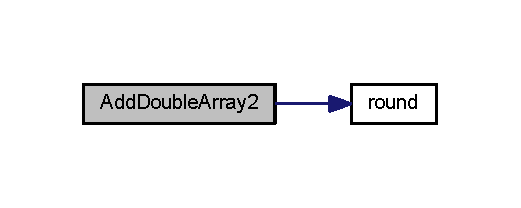
\includegraphics[width=250pt]{doublearray_8cpp_a85218774a5ad8746e40d11332f667e6a_cgraph}
\end{center}
\end{figure}


\hypertarget{doublearray_8cpp_aa26e1056a74ba31a3081a7b63a72ae0f}{\index{doublearray.\-cpp@{doublearray.\-cpp}!Center\-Double\-Array@{Center\-Double\-Array}}
\index{Center\-Double\-Array@{Center\-Double\-Array}!doublearray.cpp@{doublearray.\-cpp}}
\subsubsection[{Center\-Double\-Array}]{\setlength{\rightskip}{0pt plus 5cm}void Center\-Double\-Array (
\begin{DoxyParamCaption}
\item[{double $\ast$\&}]{arr, }
\item[{int}]{N1, }
\item[{int}]{N2}
\end{DoxyParamCaption}
)}}\label{doublearray_8cpp_aa26e1056a74ba31a3081a7b63a72ae0f}


Definition at line 743 of file doublearray.\-cpp.



Here is the call graph for this function\-:
\nopagebreak
\begin{figure}[H]
\begin{center}
\leavevmode
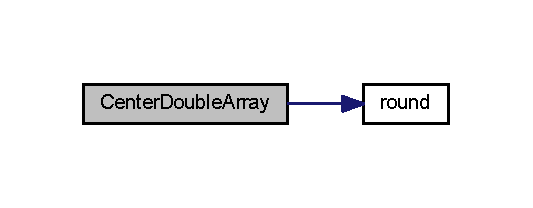
\includegraphics[width=256pt]{doublearray_8cpp_aa26e1056a74ba31a3081a7b63a72ae0f_cgraph}
\end{center}
\end{figure}


\hypertarget{doublearray_8cpp_a68d66dd58f1de9c0778ff6f80ab10dea}{\index{doublearray.\-cpp@{doublearray.\-cpp}!Clip\-Double\-Array\-Using\-Z\-Score@{Clip\-Double\-Array\-Using\-Z\-Score}}
\index{Clip\-Double\-Array\-Using\-Z\-Score@{Clip\-Double\-Array\-Using\-Z\-Score}!doublearray.cpp@{doublearray.\-cpp}}
\subsubsection[{Clip\-Double\-Array\-Using\-Z\-Score}]{\setlength{\rightskip}{0pt plus 5cm}void Clip\-Double\-Array\-Using\-Z\-Score (
\begin{DoxyParamCaption}
\item[{double $\ast$\&}]{arr, }
\item[{double}]{mean, }
\item[{double}]{sigma, }
\item[{double}]{Z\-Score, }
\item[{int}]{N1, }
\item[{int}]{N2}
\end{DoxyParamCaption}
)}}\label{doublearray_8cpp_a68d66dd58f1de9c0778ff6f80ab10dea}


Definition at line 609 of file doublearray.\-cpp.

\hypertarget{doublearray_8cpp_a05c67876c6eb936bce9e5d33ca8401ca}{\index{doublearray.\-cpp@{doublearray.\-cpp}!Close\-Double\-Array@{Close\-Double\-Array}}
\index{Close\-Double\-Array@{Close\-Double\-Array}!doublearray.cpp@{doublearray.\-cpp}}
\subsubsection[{Close\-Double\-Array}]{\setlength{\rightskip}{0pt plus 5cm}void Close\-Double\-Array (
\begin{DoxyParamCaption}
\item[{double $\ast$\&}]{arr, }
\item[{int}]{N1, }
\item[{int}]{N2}
\end{DoxyParamCaption}
)}}\label{doublearray_8cpp_a05c67876c6eb936bce9e5d33ca8401ca}


Definition at line 695 of file doublearray.\-cpp.



Here is the call graph for this function\-:
\nopagebreak
\begin{figure}[H]
\begin{center}
\leavevmode
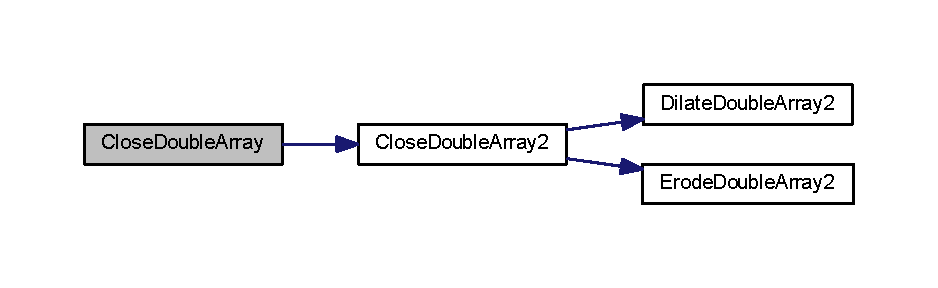
\includegraphics[width=350pt]{doublearray_8cpp_a05c67876c6eb936bce9e5d33ca8401ca_cgraph}
\end{center}
\end{figure}


\hypertarget{doublearray_8cpp_a94a0f3e08aecc9874677682fd5c982d2}{\index{doublearray.\-cpp@{doublearray.\-cpp}!Close\-Double\-Array2@{Close\-Double\-Array2}}
\index{Close\-Double\-Array2@{Close\-Double\-Array2}!doublearray.cpp@{doublearray.\-cpp}}
\subsubsection[{Close\-Double\-Array2}]{\setlength{\rightskip}{0pt plus 5cm}void Close\-Double\-Array2 (
\begin{DoxyParamCaption}
\item[{double $\ast$}]{arr, }
\item[{double $\ast$\&}]{arr\-Out, }
\item[{int}]{N1, }
\item[{int}]{N2}
\end{DoxyParamCaption}
)}}\label{doublearray_8cpp_a94a0f3e08aecc9874677682fd5c982d2}


Definition at line 654 of file doublearray.\-cpp.



Here is the call graph for this function\-:
\nopagebreak
\begin{figure}[H]
\begin{center}
\leavevmode
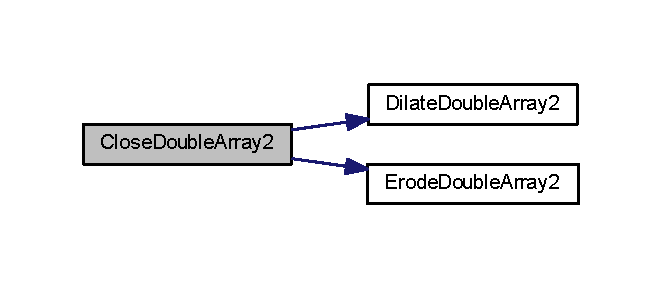
\includegraphics[width=318pt]{doublearray_8cpp_a94a0f3e08aecc9874677682fd5c982d2_cgraph}
\end{center}
\end{figure}


\hypertarget{doublearray_8cpp_a52a21b223027d4451e19d0ba82ee7824}{\index{doublearray.\-cpp@{doublearray.\-cpp}!Convolve\-Double\-Arrays@{Convolve\-Double\-Arrays}}
\index{Convolve\-Double\-Arrays@{Convolve\-Double\-Arrays}!doublearray.cpp@{doublearray.\-cpp}}
\subsubsection[{Convolve\-Double\-Arrays}]{\setlength{\rightskip}{0pt plus 5cm}void Convolve\-Double\-Arrays (
\begin{DoxyParamCaption}
\item[{double $\ast$}]{arr1, }
\item[{double $\ast$}]{arr2, }
\item[{double $\ast$\&}]{arr3, }
\item[{int}]{N1, }
\item[{int}]{N2, }
\item[{int}]{M1, }
\item[{int}]{M2}
\end{DoxyParamCaption}
)}}\label{doublearray_8cpp_a52a21b223027d4451e19d0ba82ee7824}


Definition at line 540 of file doublearray.\-cpp.

\hypertarget{doublearray_8cpp_af5ae02f38013ee530b629f5e2cbb4093}{\index{doublearray.\-cpp@{doublearray.\-cpp}!Copy\-Double\-To\-Double\-Array@{Copy\-Double\-To\-Double\-Array}}
\index{Copy\-Double\-To\-Double\-Array@{Copy\-Double\-To\-Double\-Array}!doublearray.cpp@{doublearray.\-cpp}}
\subsubsection[{Copy\-Double\-To\-Double\-Array}]{\setlength{\rightskip}{0pt plus 5cm}void Copy\-Double\-To\-Double\-Array (
\begin{DoxyParamCaption}
\item[{double $\ast$}]{arr, }
\item[{double $\ast$\&}]{arr\-Out, }
\item[{int}]{N1, }
\item[{int}]{N2}
\end{DoxyParamCaption}
)}}\label{doublearray_8cpp_af5ae02f38013ee530b629f5e2cbb4093}


Definition at line 176 of file doublearray.\-cpp.

\hypertarget{doublearray_8cpp_accc37377f8bbbac93ac42802726741b5}{\index{doublearray.\-cpp@{doublearray.\-cpp}!Dilate\-Double\-Array@{Dilate\-Double\-Array}}
\index{Dilate\-Double\-Array@{Dilate\-Double\-Array}!doublearray.cpp@{doublearray.\-cpp}}
\subsubsection[{Dilate\-Double\-Array}]{\setlength{\rightskip}{0pt plus 5cm}void Dilate\-Double\-Array (
\begin{DoxyParamCaption}
\item[{double $\ast$\&}]{arr, }
\item[{int}]{N1, }
\item[{int}]{N2}
\end{DoxyParamCaption}
)}}\label{doublearray_8cpp_accc37377f8bbbac93ac42802726741b5}


Definition at line 725 of file doublearray.\-cpp.



Here is the call graph for this function\-:
\nopagebreak
\begin{figure}[H]
\begin{center}
\leavevmode
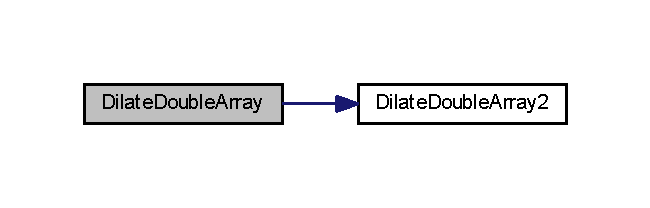
\includegraphics[width=312pt]{doublearray_8cpp_accc37377f8bbbac93ac42802726741b5_cgraph}
\end{center}
\end{figure}


\hypertarget{doublearray_8cpp_a4ae6098a7845fac0944ad664cb1abf79}{\index{doublearray.\-cpp@{doublearray.\-cpp}!Dilate\-Double\-Array2@{Dilate\-Double\-Array2}}
\index{Dilate\-Double\-Array2@{Dilate\-Double\-Array2}!doublearray.cpp@{doublearray.\-cpp}}
\subsubsection[{Dilate\-Double\-Array2}]{\setlength{\rightskip}{0pt plus 5cm}void Dilate\-Double\-Array2 (
\begin{DoxyParamCaption}
\item[{double $\ast$}]{arr, }
\item[{double $\ast$\&}]{arr\-Out, }
\item[{int}]{N1, }
\item[{int}]{N2}
\end{DoxyParamCaption}
)}}\label{doublearray_8cpp_a4ae6098a7845fac0944ad664cb1abf79}


Definition at line 798 of file doublearray.\-cpp.

\hypertarget{doublearray_8cpp_a04e473474ee3f5ab5d0c2591e1ee83d7}{\index{doublearray.\-cpp@{doublearray.\-cpp}!Display\-Double\-Array@{Display\-Double\-Array}}
\index{Display\-Double\-Array@{Display\-Double\-Array}!doublearray.cpp@{doublearray.\-cpp}}
\subsubsection[{Display\-Double\-Array}]{\setlength{\rightskip}{0pt plus 5cm}void Display\-Double\-Array (
\begin{DoxyParamCaption}
\item[{double $\ast$}]{arr, }
\item[{int}]{R\-O\-W, }
\item[{int}]{C\-O\-L}
\end{DoxyParamCaption}
)}}\label{doublearray_8cpp_a04e473474ee3f5ab5d0c2591e1ee83d7}


Definition at line 713 of file doublearray.\-cpp.

\hypertarget{doublearray_8cpp_ac53c7e23c21938b1554e363ea46fb9ef}{\index{doublearray.\-cpp@{doublearray.\-cpp}!Divide\-Double\-Arrays@{Divide\-Double\-Arrays}}
\index{Divide\-Double\-Arrays@{Divide\-Double\-Arrays}!doublearray.cpp@{doublearray.\-cpp}}
\subsubsection[{Divide\-Double\-Arrays}]{\setlength{\rightskip}{0pt plus 5cm}void Divide\-Double\-Arrays (
\begin{DoxyParamCaption}
\item[{double $\ast$}]{image1, }
\item[{double $\ast$}]{image2, }
\item[{double $\ast$\&}]{image\-Out, }
\item[{int}]{N1, }
\item[{int}]{N2}
\end{DoxyParamCaption}
)}}\label{doublearray_8cpp_ac53c7e23c21938b1554e363ea46fb9ef}


Definition at line 93 of file doublearray.\-cpp.

\hypertarget{doublearray_8cpp_a4ef5c8e4ce7b4089ed2b89dc1d9c4e60}{\index{doublearray.\-cpp@{doublearray.\-cpp}!Draw\-Line\-In\-Double\-Array@{Draw\-Line\-In\-Double\-Array}}
\index{Draw\-Line\-In\-Double\-Array@{Draw\-Line\-In\-Double\-Array}!doublearray.cpp@{doublearray.\-cpp}}
\subsubsection[{Draw\-Line\-In\-Double\-Array}]{\setlength{\rightskip}{0pt plus 5cm}void Draw\-Line\-In\-Double\-Array (
\begin{DoxyParamCaption}
\item[{double $\ast$\&}]{arr, }
\item[{int}]{N1, }
\item[{int}]{N2, }
\item[{double}]{x1, }
\item[{double}]{y1, }
\item[{double}]{x2, }
\item[{double}]{y2, }
\item[{double}]{val}
\end{DoxyParamCaption}
)}}\label{doublearray_8cpp_a4ef5c8e4ce7b4089ed2b89dc1d9c4e60}


Definition at line 358 of file doublearray.\-cpp.



Here is the call graph for this function\-:
\nopagebreak
\begin{figure}[H]
\begin{center}
\leavevmode
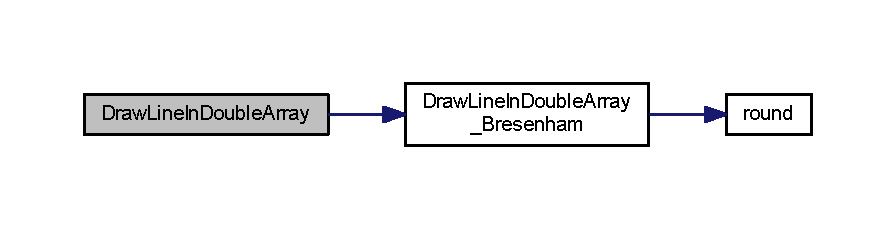
\includegraphics[width=350pt]{doublearray_8cpp_a4ef5c8e4ce7b4089ed2b89dc1d9c4e60_cgraph}
\end{center}
\end{figure}


\hypertarget{doublearray_8cpp_aefad9e5bcdd81f7f4e4cf0d694fc9dfb}{\index{doublearray.\-cpp@{doublearray.\-cpp}!Draw\-Line\-In\-Double\-Array\-\_\-\-Bresenham@{Draw\-Line\-In\-Double\-Array\-\_\-\-Bresenham}}
\index{Draw\-Line\-In\-Double\-Array\-\_\-\-Bresenham@{Draw\-Line\-In\-Double\-Array\-\_\-\-Bresenham}!doublearray.cpp@{doublearray.\-cpp}}
\subsubsection[{Draw\-Line\-In\-Double\-Array\-\_\-\-Bresenham}]{\setlength{\rightskip}{0pt plus 5cm}void Draw\-Line\-In\-Double\-Array\-\_\-\-Bresenham (
\begin{DoxyParamCaption}
\item[{double $\ast$\&}]{arr, }
\item[{int}]{N1, }
\item[{int}]{N2, }
\item[{double}]{x1, }
\item[{double}]{y1, }
\item[{double}]{x2, }
\item[{double}]{y2, }
\item[{double}]{val}
\end{DoxyParamCaption}
)}}\label{doublearray_8cpp_aefad9e5bcdd81f7f4e4cf0d694fc9dfb}


Definition at line 404 of file doublearray.\-cpp.



Here is the call graph for this function\-:
\nopagebreak
\begin{figure}[H]
\begin{center}
\leavevmode
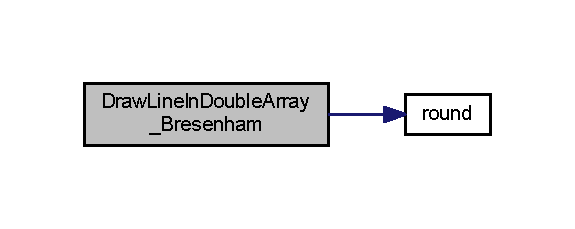
\includegraphics[width=276pt]{doublearray_8cpp_aefad9e5bcdd81f7f4e4cf0d694fc9dfb_cgraph}
\end{center}
\end{figure}


\hypertarget{doublearray_8cpp_af26847f3b9f9980d624eb02b8c1212d7}{\index{doublearray.\-cpp@{doublearray.\-cpp}!Draw\-Line\-In\-Double\-Array\-\_\-\-Bresenham\-\_\-\-N@{Draw\-Line\-In\-Double\-Array\-\_\-\-Bresenham\-\_\-\-N}}
\index{Draw\-Line\-In\-Double\-Array\-\_\-\-Bresenham\-\_\-\-N@{Draw\-Line\-In\-Double\-Array\-\_\-\-Bresenham\-\_\-\-N}!doublearray.cpp@{doublearray.\-cpp}}
\subsubsection[{Draw\-Line\-In\-Double\-Array\-\_\-\-Bresenham\-\_\-\-N}]{\setlength{\rightskip}{0pt plus 5cm}void Draw\-Line\-In\-Double\-Array\-\_\-\-Bresenham\-\_\-\-N (
\begin{DoxyParamCaption}
\item[{double $\ast$\&}]{arr, }
\item[{int}]{N1, }
\item[{int}]{N2, }
\item[{double}]{x1, }
\item[{double}]{y1, }
\item[{double}]{x2, }
\item[{double}]{y2, }
\item[{double}]{val, }
\item[{int}]{N}
\end{DoxyParamCaption}
)}}\label{doublearray_8cpp_af26847f3b9f9980d624eb02b8c1212d7}


Definition at line 372 of file doublearray.\-cpp.



Here is the call graph for this function\-:
\nopagebreak
\begin{figure}[H]
\begin{center}
\leavevmode
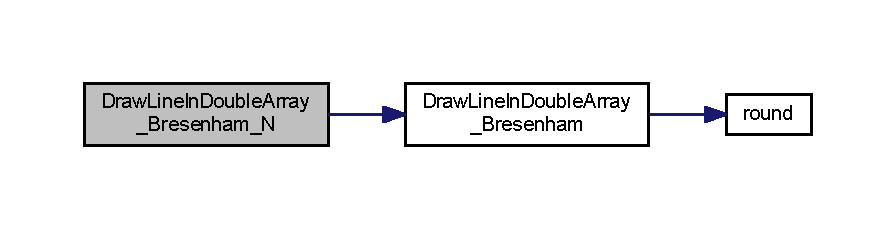
\includegraphics[width=350pt]{doublearray_8cpp_af26847f3b9f9980d624eb02b8c1212d7_cgraph}
\end{center}
\end{figure}


\hypertarget{doublearray_8cpp_a73c1563b450e254d24e80b7292b54ea5}{\index{doublearray.\-cpp@{doublearray.\-cpp}!Draw\-Line\-In\-Double\-Array\-\_\-\-D\-D\-A@{Draw\-Line\-In\-Double\-Array\-\_\-\-D\-D\-A}}
\index{Draw\-Line\-In\-Double\-Array\-\_\-\-D\-D\-A@{Draw\-Line\-In\-Double\-Array\-\_\-\-D\-D\-A}!doublearray.cpp@{doublearray.\-cpp}}
\subsubsection[{Draw\-Line\-In\-Double\-Array\-\_\-\-D\-D\-A}]{\setlength{\rightskip}{0pt plus 5cm}void Draw\-Line\-In\-Double\-Array\-\_\-\-D\-D\-A (
\begin{DoxyParamCaption}
\item[{double $\ast$\&}]{arr, }
\item[{int}]{N1, }
\item[{int}]{N2, }
\item[{double}]{x1, }
\item[{double}]{y1, }
\item[{double}]{x2, }
\item[{double}]{y2, }
\item[{double}]{val}
\end{DoxyParamCaption}
)}}\label{doublearray_8cpp_a73c1563b450e254d24e80b7292b54ea5}


Definition at line 182 of file doublearray.\-cpp.



Here is the call graph for this function\-:
\nopagebreak
\begin{figure}[H]
\begin{center}
\leavevmode
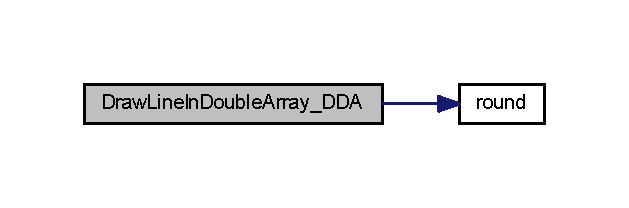
\includegraphics[width=302pt]{doublearray_8cpp_a73c1563b450e254d24e80b7292b54ea5_cgraph}
\end{center}
\end{figure}


\hypertarget{doublearray_8cpp_a452d0462be3b1c1229d65dd45c54298c}{\index{doublearray.\-cpp@{doublearray.\-cpp}!Draw\-Line\-In\-Double\-Array\-\_\-\-D\-D\-A\-\_\-\-N@{Draw\-Line\-In\-Double\-Array\-\_\-\-D\-D\-A\-\_\-\-N}}
\index{Draw\-Line\-In\-Double\-Array\-\_\-\-D\-D\-A\-\_\-\-N@{Draw\-Line\-In\-Double\-Array\-\_\-\-D\-D\-A\-\_\-\-N}!doublearray.cpp@{doublearray.\-cpp}}
\subsubsection[{Draw\-Line\-In\-Double\-Array\-\_\-\-D\-D\-A\-\_\-\-N}]{\setlength{\rightskip}{0pt plus 5cm}void Draw\-Line\-In\-Double\-Array\-\_\-\-D\-D\-A\-\_\-\-N (
\begin{DoxyParamCaption}
\item[{double $\ast$\&}]{arr, }
\item[{int}]{N1, }
\item[{int}]{N2, }
\item[{double}]{x1, }
\item[{double}]{y1, }
\item[{double}]{x2, }
\item[{double}]{y2, }
\item[{double}]{val, }
\item[{int}]{N}
\end{DoxyParamCaption}
)}}\label{doublearray_8cpp_a452d0462be3b1c1229d65dd45c54298c}


Definition at line 470 of file doublearray.\-cpp.



Here is the call graph for this function\-:
\nopagebreak
\begin{figure}[H]
\begin{center}
\leavevmode
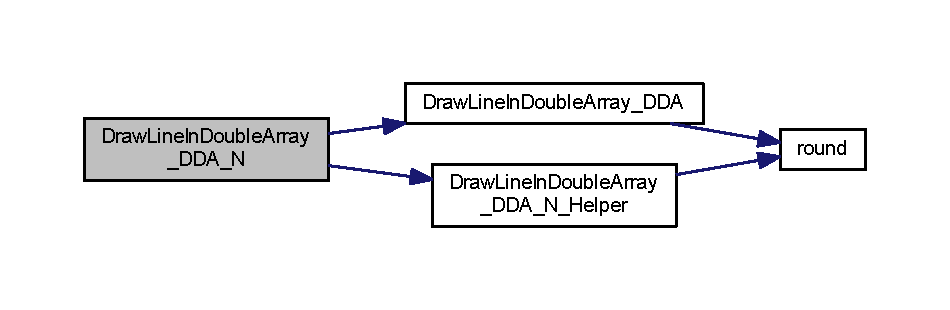
\includegraphics[width=350pt]{doublearray_8cpp_a452d0462be3b1c1229d65dd45c54298c_cgraph}
\end{center}
\end{figure}


\hypertarget{doublearray_8cpp_acd3ed79a855f210de95c5202c5942756}{\index{doublearray.\-cpp@{doublearray.\-cpp}!Draw\-Line\-In\-Double\-Array\-\_\-\-D\-D\-A\-\_\-\-N\-\_\-\-Helper@{Draw\-Line\-In\-Double\-Array\-\_\-\-D\-D\-A\-\_\-\-N\-\_\-\-Helper}}
\index{Draw\-Line\-In\-Double\-Array\-\_\-\-D\-D\-A\-\_\-\-N\-\_\-\-Helper@{Draw\-Line\-In\-Double\-Array\-\_\-\-D\-D\-A\-\_\-\-N\-\_\-\-Helper}!doublearray.cpp@{doublearray.\-cpp}}
\subsubsection[{Draw\-Line\-In\-Double\-Array\-\_\-\-D\-D\-A\-\_\-\-N\-\_\-\-Helper}]{\setlength{\rightskip}{0pt plus 5cm}void Draw\-Line\-In\-Double\-Array\-\_\-\-D\-D\-A\-\_\-\-N\-\_\-\-Helper (
\begin{DoxyParamCaption}
\item[{double $\ast$\&}]{arr, }
\item[{int}]{N1, }
\item[{int}]{N2, }
\item[{double}]{x1, }
\item[{double}]{y1, }
\item[{double}]{x2, }
\item[{double}]{y2, }
\item[{double}]{val, }
\item[{int}]{dn}
\end{DoxyParamCaption}
)}}\label{doublearray_8cpp_acd3ed79a855f210de95c5202c5942756}


Definition at line 484 of file doublearray.\-cpp.



Here is the call graph for this function\-:
\nopagebreak
\begin{figure}[H]
\begin{center}
\leavevmode
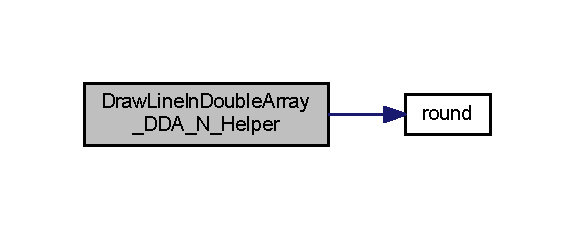
\includegraphics[width=276pt]{doublearray_8cpp_acd3ed79a855f210de95c5202c5942756_cgraph}
\end{center}
\end{figure}


\hypertarget{doublearray_8cpp_a500bba1190ba419fdab522f1dc7ab0aa}{\index{doublearray.\-cpp@{doublearray.\-cpp}!Draw\-Line\-In\-Double\-Array\-\_\-\-N@{Draw\-Line\-In\-Double\-Array\-\_\-\-N}}
\index{Draw\-Line\-In\-Double\-Array\-\_\-\-N@{Draw\-Line\-In\-Double\-Array\-\_\-\-N}!doublearray.cpp@{doublearray.\-cpp}}
\subsubsection[{Draw\-Line\-In\-Double\-Array\-\_\-\-N}]{\setlength{\rightskip}{0pt plus 5cm}void Draw\-Line\-In\-Double\-Array\-\_\-\-N (
\begin{DoxyParamCaption}
\item[{double $\ast$\&}]{arr, }
\item[{int}]{N1, }
\item[{int}]{N2, }
\item[{double}]{x1, }
\item[{double}]{y1, }
\item[{double}]{x2, }
\item[{double}]{y2, }
\item[{double}]{val, }
\item[{int}]{N}
\end{DoxyParamCaption}
)}}\label{doublearray_8cpp_a500bba1190ba419fdab522f1dc7ab0aa}


Definition at line 363 of file doublearray.\-cpp.



Here is the call graph for this function\-:
\nopagebreak
\begin{figure}[H]
\begin{center}
\leavevmode
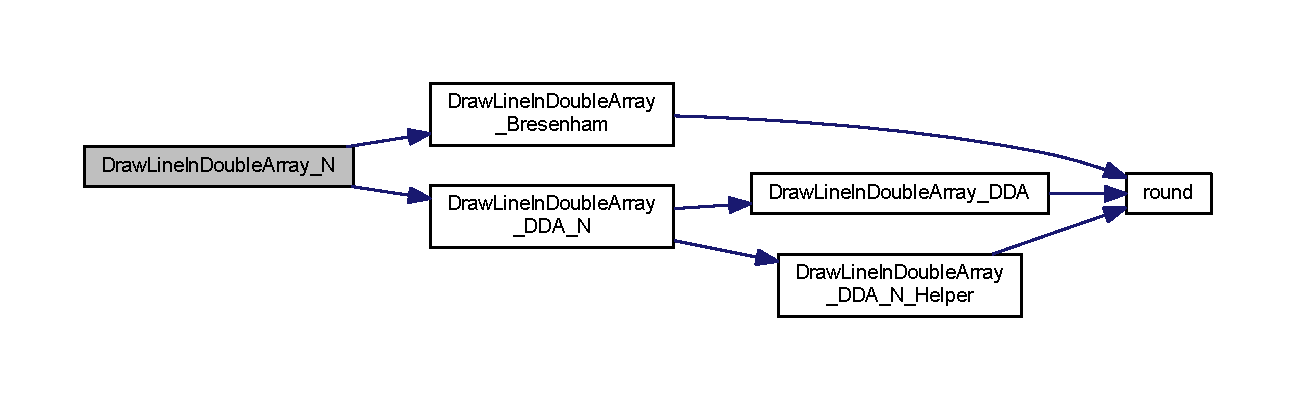
\includegraphics[width=350pt]{doublearray_8cpp_a500bba1190ba419fdab522f1dc7ab0aa_cgraph}
\end{center}
\end{figure}


\hypertarget{doublearray_8cpp_ae4e3b80458efff3f8e6756b8b9cc27a3}{\index{doublearray.\-cpp@{doublearray.\-cpp}!Edges\-Laplacian\-Double\-Array@{Edges\-Laplacian\-Double\-Array}}
\index{Edges\-Laplacian\-Double\-Array@{Edges\-Laplacian\-Double\-Array}!doublearray.cpp@{doublearray.\-cpp}}
\subsubsection[{Edges\-Laplacian\-Double\-Array}]{\setlength{\rightskip}{0pt plus 5cm}void Edges\-Laplacian\-Double\-Array (
\begin{DoxyParamCaption}
\item[{double $\ast$}]{arr, }
\item[{double $\ast$\&}]{arr\-Out, }
\item[{int}]{N1, }
\item[{int}]{N2}
\end{DoxyParamCaption}
)}}\label{doublearray_8cpp_ae4e3b80458efff3f8e6756b8b9cc27a3}


Definition at line 26 of file doublearray.\-cpp.



Here is the call graph for this function\-:
\nopagebreak
\begin{figure}[H]
\begin{center}
\leavevmode
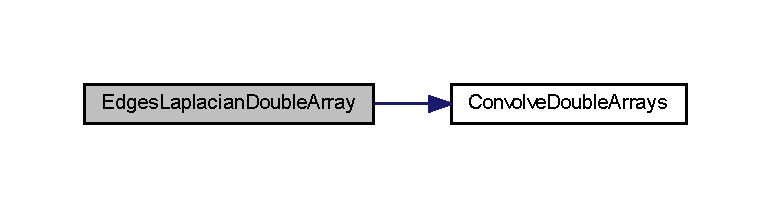
\includegraphics[width=350pt]{doublearray_8cpp_ae4e3b80458efff3f8e6756b8b9cc27a3_cgraph}
\end{center}
\end{figure}


\hypertarget{doublearray_8cpp_af3f1295a7e4a75c43907db64e40c2400}{\index{doublearray.\-cpp@{doublearray.\-cpp}!Edges\-Sobel\-Double\-Array@{Edges\-Sobel\-Double\-Array}}
\index{Edges\-Sobel\-Double\-Array@{Edges\-Sobel\-Double\-Array}!doublearray.cpp@{doublearray.\-cpp}}
\subsubsection[{Edges\-Sobel\-Double\-Array}]{\setlength{\rightskip}{0pt plus 5cm}void Edges\-Sobel\-Double\-Array (
\begin{DoxyParamCaption}
\item[{double $\ast$}]{arr, }
\item[{double $\ast$\&}]{arr\-Out, }
\item[{int}]{N1, }
\item[{int}]{N2}
\end{DoxyParamCaption}
)}}\label{doublearray_8cpp_af3f1295a7e4a75c43907db64e40c2400}


Definition at line 36 of file doublearray.\-cpp.



Here is the call graph for this function\-:
\nopagebreak
\begin{figure}[H]
\begin{center}
\leavevmode
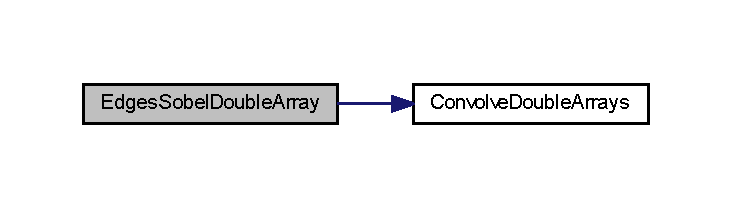
\includegraphics[width=350pt]{doublearray_8cpp_af3f1295a7e4a75c43907db64e40c2400_cgraph}
\end{center}
\end{figure}


\hypertarget{doublearray_8cpp_ac025547a3c77be19835c883ce233d902}{\index{doublearray.\-cpp@{doublearray.\-cpp}!Erode\-Double\-Array@{Erode\-Double\-Array}}
\index{Erode\-Double\-Array@{Erode\-Double\-Array}!doublearray.cpp@{doublearray.\-cpp}}
\subsubsection[{Erode\-Double\-Array}]{\setlength{\rightskip}{0pt plus 5cm}void Erode\-Double\-Array (
\begin{DoxyParamCaption}
\item[{double $\ast$\&}]{arr, }
\item[{int}]{N1, }
\item[{int}]{N2}
\end{DoxyParamCaption}
)}}\label{doublearray_8cpp_ac025547a3c77be19835c883ce233d902}


Definition at line 734 of file doublearray.\-cpp.



Here is the call graph for this function\-:
\nopagebreak
\begin{figure}[H]
\begin{center}
\leavevmode
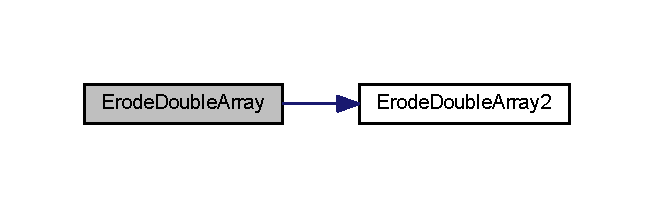
\includegraphics[width=314pt]{doublearray_8cpp_ac025547a3c77be19835c883ce233d902_cgraph}
\end{center}
\end{figure}


\hypertarget{doublearray_8cpp_a05656fb702a00b8149dfa78bfae2582c}{\index{doublearray.\-cpp@{doublearray.\-cpp}!Erode\-Double\-Array2@{Erode\-Double\-Array2}}
\index{Erode\-Double\-Array2@{Erode\-Double\-Array2}!doublearray.cpp@{doublearray.\-cpp}}
\subsubsection[{Erode\-Double\-Array2}]{\setlength{\rightskip}{0pt plus 5cm}void Erode\-Double\-Array2 (
\begin{DoxyParamCaption}
\item[{double $\ast$}]{arr, }
\item[{double $\ast$\&}]{arr\-Out, }
\item[{int}]{N1, }
\item[{int}]{N2}
\end{DoxyParamCaption}
)}}\label{doublearray_8cpp_a05656fb702a00b8149dfa78bfae2582c}


Definition at line 826 of file doublearray.\-cpp.

\hypertarget{doublearray_8cpp_a0901a62db5e9b8f00bb8d74b2f663061}{\index{doublearray.\-cpp@{doublearray.\-cpp}!Extend\-Double\-Array@{Extend\-Double\-Array}}
\index{Extend\-Double\-Array@{Extend\-Double\-Array}!doublearray.cpp@{doublearray.\-cpp}}
\subsubsection[{Extend\-Double\-Array}]{\setlength{\rightskip}{0pt plus 5cm}void Extend\-Double\-Array (
\begin{DoxyParamCaption}
\item[{double $\ast$}]{arr, }
\item[{double $\ast$\&}]{arr\-Out, }
\item[{double}]{x, }
\item[{double}]{y, }
\item[{int}]{N1, }
\item[{int}]{N2, }
\item[{int}]{M1, }
\item[{int}]{M2}
\end{DoxyParamCaption}
)}}\label{doublearray_8cpp_a0901a62db5e9b8f00bb8d74b2f663061}


Definition at line 905 of file doublearray.\-cpp.



Here is the call graph for this function\-:
\nopagebreak
\begin{figure}[H]
\begin{center}
\leavevmode
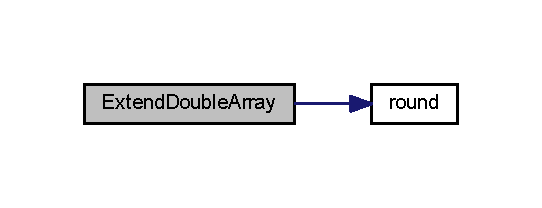
\includegraphics[width=260pt]{doublearray_8cpp_a0901a62db5e9b8f00bb8d74b2f663061_cgraph}
\end{center}
\end{figure}


\hypertarget{doublearray_8cpp_ab3052e47549b941dce4a630a7fb3c7c1}{\index{doublearray.\-cpp@{doublearray.\-cpp}!Flip\-Horizontal\-Double\-Array@{Flip\-Horizontal\-Double\-Array}}
\index{Flip\-Horizontal\-Double\-Array@{Flip\-Horizontal\-Double\-Array}!doublearray.cpp@{doublearray.\-cpp}}
\subsubsection[{Flip\-Horizontal\-Double\-Array}]{\setlength{\rightskip}{0pt plus 5cm}void Flip\-Horizontal\-Double\-Array (
\begin{DoxyParamCaption}
\item[{double $\ast$}]{arr, }
\item[{double $\ast$}]{arr\-Out, }
\item[{int}]{N1, }
\item[{int}]{N2}
\end{DoxyParamCaption}
)}}\label{doublearray_8cpp_ab3052e47549b941dce4a630a7fb3c7c1}


Definition at line 568 of file doublearray.\-cpp.

\hypertarget{doublearray_8cpp_a511dff95c8f666b13a0d680d5c69c428}{\index{doublearray.\-cpp@{doublearray.\-cpp}!Flip\-Vertical\-Double\-Array@{Flip\-Vertical\-Double\-Array}}
\index{Flip\-Vertical\-Double\-Array@{Flip\-Vertical\-Double\-Array}!doublearray.cpp@{doublearray.\-cpp}}
\subsubsection[{Flip\-Vertical\-Double\-Array}]{\setlength{\rightskip}{0pt plus 5cm}void Flip\-Vertical\-Double\-Array (
\begin{DoxyParamCaption}
\item[{double $\ast$}]{arr, }
\item[{double $\ast$}]{arr\-Out, }
\item[{int}]{N1, }
\item[{int}]{N2}
\end{DoxyParamCaption}
)}}\label{doublearray_8cpp_a511dff95c8f666b13a0d680d5c69c428}


Definition at line 561 of file doublearray.\-cpp.

\hypertarget{doublearray_8cpp_a97bb928aff6f1afad8b0dfa3d703535e}{\index{doublearray.\-cpp@{doublearray.\-cpp}!Locate\-Min\-Max\-Double\-Array@{Locate\-Min\-Max\-Double\-Array}}
\index{Locate\-Min\-Max\-Double\-Array@{Locate\-Min\-Max\-Double\-Array}!doublearray.cpp@{doublearray.\-cpp}}
\subsubsection[{Locate\-Min\-Max\-Double\-Array}]{\setlength{\rightskip}{0pt plus 5cm}void Locate\-Min\-Max\-Double\-Array (
\begin{DoxyParamCaption}
\item[{double $\ast$}]{arr, }
\item[{int}]{N1, }
\item[{int}]{N2, }
\item[{double \&}]{min1, }
\item[{double \&}]{max1, }
\item[{int \&}]{mini, }
\item[{int \&}]{minj, }
\item[{int \&}]{maxi, }
\item[{int \&}]{maxj}
\end{DoxyParamCaption}
)}}\label{doublearray_8cpp_a97bb928aff6f1afad8b0dfa3d703535e}


Definition at line 576 of file doublearray.\-cpp.

\hypertarget{doublearray_8cpp_a6641c67e5167774ccfcd0beb47a4df1b}{\index{doublearray.\-cpp@{doublearray.\-cpp}!Log\-Double\-Array@{Log\-Double\-Array}}
\index{Log\-Double\-Array@{Log\-Double\-Array}!doublearray.cpp@{doublearray.\-cpp}}
\subsubsection[{Log\-Double\-Array}]{\setlength{\rightskip}{0pt plus 5cm}void Log\-Double\-Array (
\begin{DoxyParamCaption}
\item[{double $\ast$}]{arr, }
\item[{int}]{N1, }
\item[{int}]{N2}
\end{DoxyParamCaption}
)}}\label{doublearray_8cpp_a6641c67e5167774ccfcd0beb47a4df1b}


Definition at line 133 of file doublearray.\-cpp.



Here is the call graph for this function\-:
\nopagebreak
\begin{figure}[H]
\begin{center}
\leavevmode
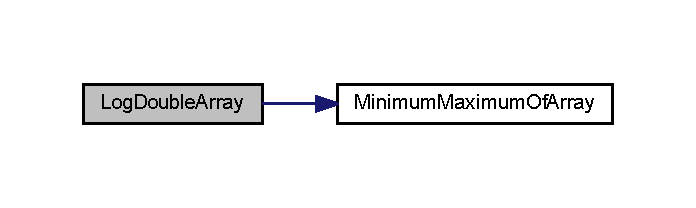
\includegraphics[width=334pt]{doublearray_8cpp_a6641c67e5167774ccfcd0beb47a4df1b_cgraph}
\end{center}
\end{figure}


\hypertarget{doublearray_8cpp_a05115ec8293000a3163007bcf88ee956}{\index{doublearray.\-cpp@{doublearray.\-cpp}!Minimum\-Maximum\-Of\-Array@{Minimum\-Maximum\-Of\-Array}}
\index{Minimum\-Maximum\-Of\-Array@{Minimum\-Maximum\-Of\-Array}!doublearray.cpp@{doublearray.\-cpp}}
\subsubsection[{Minimum\-Maximum\-Of\-Array}]{\setlength{\rightskip}{0pt plus 5cm}void Minimum\-Maximum\-Of\-Array (
\begin{DoxyParamCaption}
\item[{double $\ast$}]{arr, }
\item[{int}]{N1, }
\item[{int}]{N2, }
\item[{double \&}]{min1, }
\item[{double \&}]{max1}
\end{DoxyParamCaption}
)}}\label{doublearray_8cpp_a05115ec8293000a3163007bcf88ee956}


Definition at line 123 of file doublearray.\-cpp.

\hypertarget{doublearray_8cpp_a086d2dccfe8cbef8a954881b6aae65c1}{\index{doublearray.\-cpp@{doublearray.\-cpp}!Multiply\-Double\-Arrays@{Multiply\-Double\-Arrays}}
\index{Multiply\-Double\-Arrays@{Multiply\-Double\-Arrays}!doublearray.cpp@{doublearray.\-cpp}}
\subsubsection[{Multiply\-Double\-Arrays}]{\setlength{\rightskip}{0pt plus 5cm}void Multiply\-Double\-Arrays (
\begin{DoxyParamCaption}
\item[{double $\ast$}]{arr1, }
\item[{double $\ast$}]{arr2, }
\item[{double $\ast$\&}]{arr\-Out, }
\item[{int}]{N1, }
\item[{int}]{N2, }
\item[{int}]{N3}
\end{DoxyParamCaption}
)}}\label{doublearray_8cpp_a086d2dccfe8cbef8a954881b6aae65c1}


Definition at line 682 of file doublearray.\-cpp.

\hypertarget{doublearray_8cpp_a8199fd9d2030481ef8a987aef3b79634}{\index{doublearray.\-cpp@{doublearray.\-cpp}!Open\-Double\-Array@{Open\-Double\-Array}}
\index{Open\-Double\-Array@{Open\-Double\-Array}!doublearray.cpp@{doublearray.\-cpp}}
\subsubsection[{Open\-Double\-Array}]{\setlength{\rightskip}{0pt plus 5cm}void Open\-Double\-Array (
\begin{DoxyParamCaption}
\item[{double $\ast$\&}]{arr, }
\item[{int}]{N1, }
\item[{int}]{N2}
\end{DoxyParamCaption}
)}}\label{doublearray_8cpp_a8199fd9d2030481ef8a987aef3b79634}


Definition at line 704 of file doublearray.\-cpp.



Here is the call graph for this function\-:
\nopagebreak
\begin{figure}[H]
\begin{center}
\leavevmode
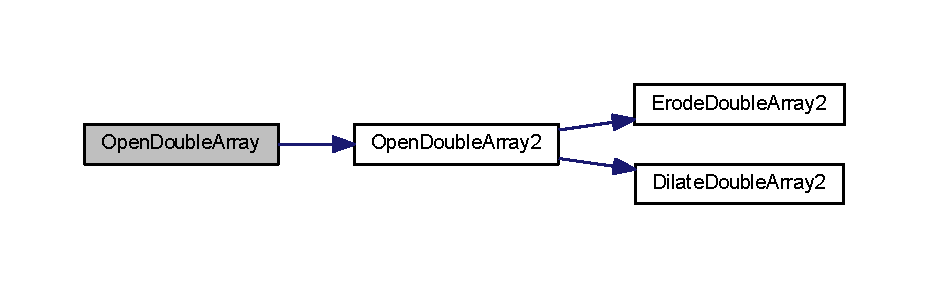
\includegraphics[width=350pt]{doublearray_8cpp_a8199fd9d2030481ef8a987aef3b79634_cgraph}
\end{center}
\end{figure}


\hypertarget{doublearray_8cpp_afcfc024419938e3553b330a315bc92cf}{\index{doublearray.\-cpp@{doublearray.\-cpp}!Open\-Double\-Array2@{Open\-Double\-Array2}}
\index{Open\-Double\-Array2@{Open\-Double\-Array2}!doublearray.cpp@{doublearray.\-cpp}}
\subsubsection[{Open\-Double\-Array2}]{\setlength{\rightskip}{0pt plus 5cm}void Open\-Double\-Array2 (
\begin{DoxyParamCaption}
\item[{double $\ast$}]{arr, }
\item[{double $\ast$\&}]{arr\-Out, }
\item[{int}]{N1, }
\item[{int}]{N2}
\end{DoxyParamCaption}
)}}\label{doublearray_8cpp_afcfc024419938e3553b330a315bc92cf}


Definition at line 663 of file doublearray.\-cpp.



Here is the call graph for this function\-:
\nopagebreak
\begin{figure}[H]
\begin{center}
\leavevmode
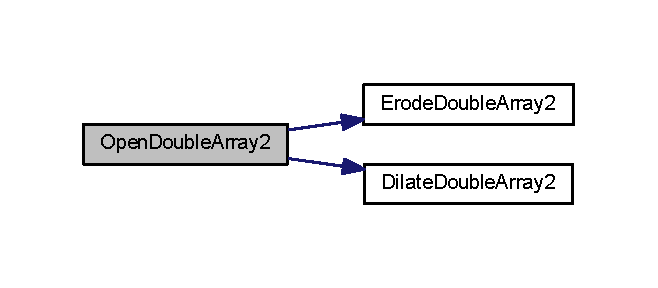
\includegraphics[width=316pt]{doublearray_8cpp_afcfc024419938e3553b330a315bc92cf_cgraph}
\end{center}
\end{figure}


\hypertarget{doublearray_8cpp_acacf2689331cb439d1bebef68a1f8552}{\index{doublearray.\-cpp@{doublearray.\-cpp}!Output\-Double\-Array\-To\-File@{Output\-Double\-Array\-To\-File}}
\index{Output\-Double\-Array\-To\-File@{Output\-Double\-Array\-To\-File}!doublearray.cpp@{doublearray.\-cpp}}
\subsubsection[{Output\-Double\-Array\-To\-File}]{\setlength{\rightskip}{0pt plus 5cm}void Output\-Double\-Array\-To\-File (
\begin{DoxyParamCaption}
\item[{char $\ast$}]{filename, }
\item[{double $\ast$}]{arr, }
\item[{int}]{N1, }
\item[{int}]{N2}
\end{DoxyParamCaption}
)}}\label{doublearray_8cpp_acacf2689331cb439d1bebef68a1f8552}


Definition at line 162 of file doublearray.\-cpp.

\hypertarget{doublearray_8cpp_a0fe1cc9dcb110c5e9936c113d23a5ee0}{\index{doublearray.\-cpp@{doublearray.\-cpp}!Paint\-By\-Numbers\-Double\-Array@{Paint\-By\-Numbers\-Double\-Array}}
\index{Paint\-By\-Numbers\-Double\-Array@{Paint\-By\-Numbers\-Double\-Array}!doublearray.cpp@{doublearray.\-cpp}}
\subsubsection[{Paint\-By\-Numbers\-Double\-Array}]{\setlength{\rightskip}{0pt plus 5cm}void Paint\-By\-Numbers\-Double\-Array (
\begin{DoxyParamCaption}
\item[{double $\ast$$\ast$}]{arrs, }
\item[{int}]{M1, }
\item[{int}]{M2, }
\item[{int $\ast$}]{labels, }
\item[{int}]{L1, }
\item[{int}]{L2, }
\item[{double $\ast$\&}]{arr, }
\item[{int \&}]{N1, }
\item[{int \&}]{N2}
\end{DoxyParamCaption}
)}}\label{doublearray_8cpp_a0fe1cc9dcb110c5e9936c113d23a5ee0}


Definition at line 12 of file doublearray.\-cpp.



Here is the call graph for this function\-:
\nopagebreak
\begin{figure}[H]
\begin{center}
\leavevmode
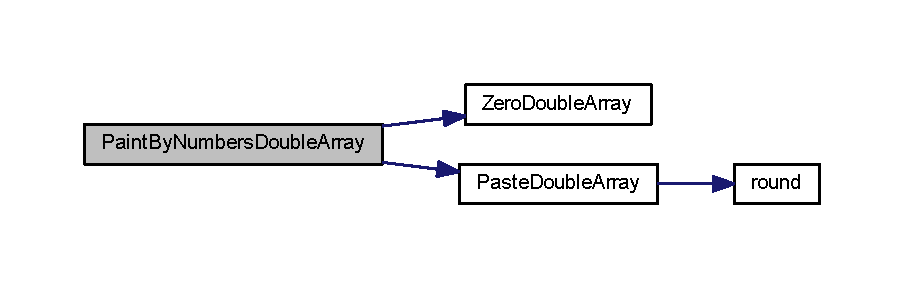
\includegraphics[width=350pt]{doublearray_8cpp_a0fe1cc9dcb110c5e9936c113d23a5ee0_cgraph}
\end{center}
\end{figure}


\hypertarget{doublearray_8cpp_abff31a105bf6a91afd998deacdbf4d44}{\index{doublearray.\-cpp@{doublearray.\-cpp}!Paste\-Double\-Array@{Paste\-Double\-Array}}
\index{Paste\-Double\-Array@{Paste\-Double\-Array}!doublearray.cpp@{doublearray.\-cpp}}
\subsubsection[{Paste\-Double\-Array}]{\setlength{\rightskip}{0pt plus 5cm}void Paste\-Double\-Array (
\begin{DoxyParamCaption}
\item[{double $\ast$\&}]{arr1, }
\item[{double $\ast$}]{arr2, }
\item[{double}]{x, }
\item[{double}]{y, }
\item[{int}]{N1, }
\item[{int}]{N2, }
\item[{int}]{M1, }
\item[{int}]{M2}
\end{DoxyParamCaption}
)}}\label{doublearray_8cpp_abff31a105bf6a91afd998deacdbf4d44}


Definition at line 891 of file doublearray.\-cpp.



Here is the call graph for this function\-:
\nopagebreak
\begin{figure}[H]
\begin{center}
\leavevmode
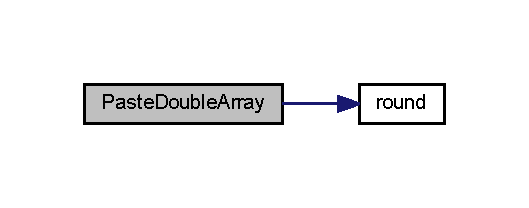
\includegraphics[width=254pt]{doublearray_8cpp_abff31a105bf6a91afd998deacdbf4d44_cgraph}
\end{center}
\end{figure}


\hypertarget{doublearray_8cpp_ae050ddd846c56f992b5c5175ed449ad8}{\index{doublearray.\-cpp@{doublearray.\-cpp}!Paste\-With\-Mask\-Double\-Array@{Paste\-With\-Mask\-Double\-Array}}
\index{Paste\-With\-Mask\-Double\-Array@{Paste\-With\-Mask\-Double\-Array}!doublearray.cpp@{doublearray.\-cpp}}
\subsubsection[{Paste\-With\-Mask\-Double\-Array}]{\setlength{\rightskip}{0pt plus 5cm}void Paste\-With\-Mask\-Double\-Array (
\begin{DoxyParamCaption}
\item[{double $\ast$\&}]{arr1, }
\item[{double $\ast$}]{arr2, }
\item[{double $\ast$}]{mask2, }
\item[{double}]{x, }
\item[{double}]{y, }
\item[{int}]{N1, }
\item[{int}]{N2, }
\item[{int}]{M1, }
\item[{int}]{M2}
\end{DoxyParamCaption}
)}}\label{doublearray_8cpp_ae050ddd846c56f992b5c5175ed449ad8}


Definition at line 595 of file doublearray.\-cpp.



Here is the call graph for this function\-:
\nopagebreak
\begin{figure}[H]
\begin{center}
\leavevmode
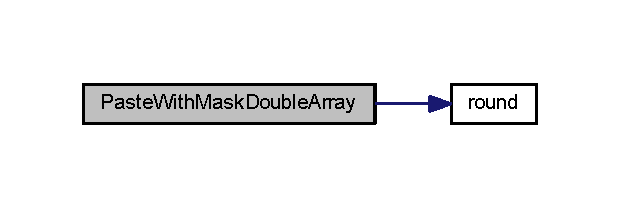
\includegraphics[width=298pt]{doublearray_8cpp_ae050ddd846c56f992b5c5175ed449ad8_cgraph}
\end{center}
\end{figure}


\hypertarget{doublearray_8cpp_aa1bd64811b94064d93db7b17b0b3daca}{\index{doublearray.\-cpp@{doublearray.\-cpp}!Polygon\-Double\-Array@{Polygon\-Double\-Array}}
\index{Polygon\-Double\-Array@{Polygon\-Double\-Array}!doublearray.cpp@{doublearray.\-cpp}}
\subsubsection[{Polygon\-Double\-Array}]{\setlength{\rightskip}{0pt plus 5cm}void Polygon\-Double\-Array (
\begin{DoxyParamCaption}
\item[{double $\ast$}]{arr, }
\item[{int}]{N1, }
\item[{int}]{N2, }
\item[{point\-Double $\ast$}]{p, }
\item[{int}]{N, }
\item[{double}]{x, }
\item[{double}]{y, }
\item[{double}]{W, }
\item[{double}]{H, }
\item[{double}]{val}
\end{DoxyParamCaption}
)}}\label{doublearray_8cpp_aa1bd64811b94064d93db7b17b0b3daca}


Definition at line 228 of file doublearray.\-cpp.



Here is the call graph for this function\-:
\nopagebreak
\begin{figure}[H]
\begin{center}
\leavevmode
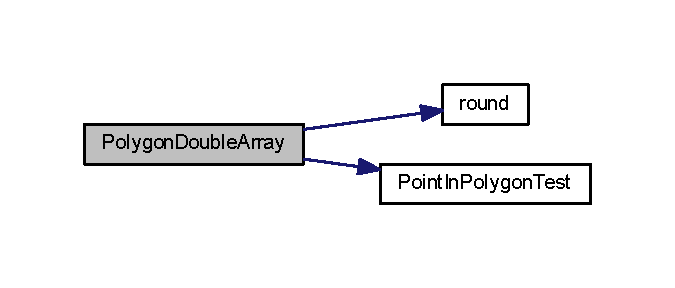
\includegraphics[width=324pt]{doublearray_8cpp_aa1bd64811b94064d93db7b17b0b3daca_cgraph}
\end{center}
\end{figure}


\hypertarget{doublearray_8cpp_a1dc3c3f85d1bb420090295c8cd7b2499}{\index{doublearray.\-cpp@{doublearray.\-cpp}!Rotate\-Angle\-Double\-Array@{Rotate\-Angle\-Double\-Array}}
\index{Rotate\-Angle\-Double\-Array@{Rotate\-Angle\-Double\-Array}!doublearray.cpp@{doublearray.\-cpp}}
\subsubsection[{Rotate\-Angle\-Double\-Array}]{\setlength{\rightskip}{0pt plus 5cm}void Rotate\-Angle\-Double\-Array (
\begin{DoxyParamCaption}
\item[{double $\ast$}]{arr, }
\item[{double $\ast$\&}]{arr\-Out, }
\item[{int}]{N1, }
\item[{int}]{N2, }
\item[{double}]{Radians}
\end{DoxyParamCaption}
)}}\label{doublearray_8cpp_a1dc3c3f85d1bb420090295c8cd7b2499}


Definition at line 250 of file doublearray.\-cpp.



Here is the call graph for this function\-:
\nopagebreak
\begin{figure}[H]
\begin{center}
\leavevmode
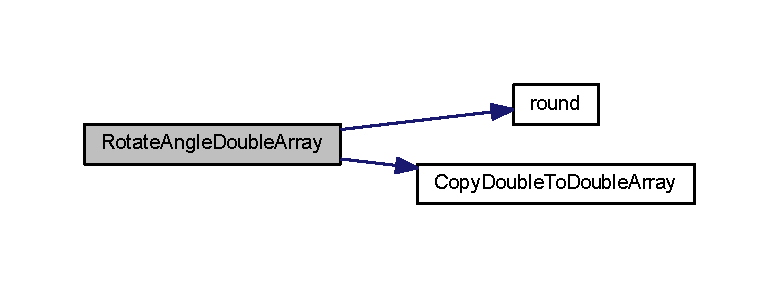
\includegraphics[width=350pt]{doublearray_8cpp_a1dc3c3f85d1bb420090295c8cd7b2499_cgraph}
\end{center}
\end{figure}


\hypertarget{doublearray_8cpp_a7c28b9f7097580074d8a9107f93fbd46}{\index{doublearray.\-cpp@{doublearray.\-cpp}!Rotate\-Left\-Double\-Array@{Rotate\-Left\-Double\-Array}}
\index{Rotate\-Left\-Double\-Array@{Rotate\-Left\-Double\-Array}!doublearray.cpp@{doublearray.\-cpp}}
\subsubsection[{Rotate\-Left\-Double\-Array}]{\setlength{\rightskip}{0pt plus 5cm}void Rotate\-Left\-Double\-Array (
\begin{DoxyParamCaption}
\item[{double $\ast$}]{arr, }
\item[{int}]{N1, }
\item[{int}]{N2, }
\item[{double $\ast$\&}]{arr\-Out, }
\item[{int \&}]{M1, }
\item[{int \&}]{M2}
\end{DoxyParamCaption}
)}}\label{doublearray_8cpp_a7c28b9f7097580074d8a9107f93fbd46}


Definition at line 347 of file doublearray.\-cpp.

\hypertarget{doublearray_8cpp_a15e257b0d36560b30c262874f54f4a8b}{\index{doublearray.\-cpp@{doublearray.\-cpp}!Rotate\-Right\-Double\-Array@{Rotate\-Right\-Double\-Array}}
\index{Rotate\-Right\-Double\-Array@{Rotate\-Right\-Double\-Array}!doublearray.cpp@{doublearray.\-cpp}}
\subsubsection[{Rotate\-Right\-Double\-Array}]{\setlength{\rightskip}{0pt plus 5cm}void Rotate\-Right\-Double\-Array (
\begin{DoxyParamCaption}
\item[{double $\ast$}]{arr, }
\item[{int}]{N1, }
\item[{int}]{N2, }
\item[{double $\ast$\&}]{arr\-Out, }
\item[{int \&}]{M1, }
\item[{int \&}]{M2}
\end{DoxyParamCaption}
)}}\label{doublearray_8cpp_a15e257b0d36560b30c262874f54f4a8b}


Definition at line 336 of file doublearray.\-cpp.

\hypertarget{doublearray_8cpp_acad3a906d768ee20770f375fbf70a952}{\index{doublearray.\-cpp@{doublearray.\-cpp}!Scale\-Double\-Array@{Scale\-Double\-Array}}
\index{Scale\-Double\-Array@{Scale\-Double\-Array}!doublearray.cpp@{doublearray.\-cpp}}
\subsubsection[{Scale\-Double\-Array}]{\setlength{\rightskip}{0pt plus 5cm}void Scale\-Double\-Array (
\begin{DoxyParamCaption}
\item[{double $\ast$\&}]{arr, }
\item[{double}]{scalar, }
\item[{int}]{N1, }
\item[{int}]{N2}
\end{DoxyParamCaption}
)}}\label{doublearray_8cpp_acad3a906d768ee20770f375fbf70a952}


Definition at line 152 of file doublearray.\-cpp.

\hypertarget{doublearray_8cpp_aa074caff8bf0bb069a3f35a7f6bb4572}{\index{doublearray.\-cpp@{doublearray.\-cpp}!Scale\-Size\-Double\-Array@{Scale\-Size\-Double\-Array}}
\index{Scale\-Size\-Double\-Array@{Scale\-Size\-Double\-Array}!doublearray.cpp@{doublearray.\-cpp}}
\subsubsection[{Scale\-Size\-Double\-Array}]{\setlength{\rightskip}{0pt plus 5cm}void Scale\-Size\-Double\-Array (
\begin{DoxyParamCaption}
\item[{double $\ast$}]{arr, }
\item[{double $\ast$\&}]{arr\-Out, }
\item[{double}]{sx, }
\item[{double}]{sy, }
\item[{int}]{N1, }
\item[{int}]{N2, }
\item[{int \&}]{M1, }
\item[{int \&}]{M2}
\end{DoxyParamCaption}
)}}\label{doublearray_8cpp_aa074caff8bf0bb069a3f35a7f6bb4572}


Definition at line 764 of file doublearray.\-cpp.



Here is the call graph for this function\-:
\nopagebreak
\begin{figure}[H]
\begin{center}
\leavevmode
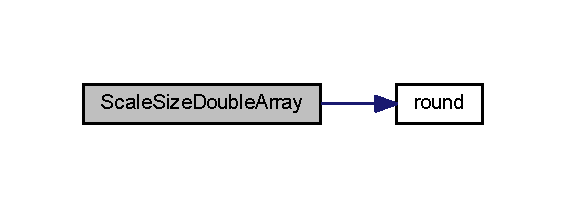
\includegraphics[width=272pt]{doublearray_8cpp_aa074caff8bf0bb069a3f35a7f6bb4572_cgraph}
\end{center}
\end{figure}


\hypertarget{doublearray_8cpp_aca71249ab74852cdecb47ad9b9e43f0f}{\index{doublearray.\-cpp@{doublearray.\-cpp}!Statistics\-Of\-Double\-Array@{Statistics\-Of\-Double\-Array}}
\index{Statistics\-Of\-Double\-Array@{Statistics\-Of\-Double\-Array}!doublearray.cpp@{doublearray.\-cpp}}
\subsubsection[{Statistics\-Of\-Double\-Array}]{\setlength{\rightskip}{0pt plus 5cm}void Statistics\-Of\-Double\-Array (
\begin{DoxyParamCaption}
\item[{double $\ast$}]{arr, }
\item[{double \&}]{mean, }
\item[{double \&}]{sigma, }
\item[{int}]{N1, }
\item[{int}]{N2}
\end{DoxyParamCaption}
)}}\label{doublearray_8cpp_aca71249ab74852cdecb47ad9b9e43f0f}


Definition at line 622 of file doublearray.\-cpp.

\hypertarget{doublearray_8cpp_ac683b719f8ce63556a6bcc0f7f306acd}{\index{doublearray.\-cpp@{doublearray.\-cpp}!Stretch\-Double\-Array@{Stretch\-Double\-Array}}
\index{Stretch\-Double\-Array@{Stretch\-Double\-Array}!doublearray.cpp@{doublearray.\-cpp}}
\subsubsection[{Stretch\-Double\-Array}]{\setlength{\rightskip}{0pt plus 5cm}void Stretch\-Double\-Array (
\begin{DoxyParamCaption}
\item[{double $\ast$\&}]{arr, }
\item[{int}]{N1, }
\item[{int}]{N2}
\end{DoxyParamCaption}
)}}\label{doublearray_8cpp_ac683b719f8ce63556a6bcc0f7f306acd}


Definition at line 62 of file doublearray.\-cpp.

\hypertarget{doublearray_8cpp_a3ae59dd7b331d1958c77d6c81391f491}{\index{doublearray.\-cpp@{doublearray.\-cpp}!Subtract\-Double\-Array2@{Subtract\-Double\-Array2}}
\index{Subtract\-Double\-Array2@{Subtract\-Double\-Array2}!doublearray.cpp@{doublearray.\-cpp}}
\subsubsection[{Subtract\-Double\-Array2}]{\setlength{\rightskip}{0pt plus 5cm}void Subtract\-Double\-Array2 (
\begin{DoxyParamCaption}
\item[{double $\ast$\&}]{arr1, }
\item[{double $\ast$}]{arr2, }
\item[{double}]{x, }
\item[{double}]{y, }
\item[{int}]{N1, }
\item[{int}]{N2, }
\item[{int}]{M1, }
\item[{int}]{M2}
\end{DoxyParamCaption}
)}}\label{doublearray_8cpp_a3ae59dd7b331d1958c77d6c81391f491}


Definition at line 877 of file doublearray.\-cpp.



Here is the call graph for this function\-:
\nopagebreak
\begin{figure}[H]
\begin{center}
\leavevmode
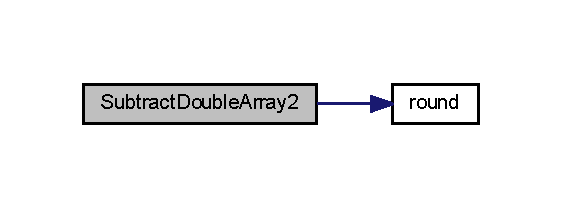
\includegraphics[width=270pt]{doublearray_8cpp_a3ae59dd7b331d1958c77d6c81391f491_cgraph}
\end{center}
\end{figure}


\hypertarget{doublearray_8cpp_aa61d08caadf680da67f5fd233fb44ecc}{\index{doublearray.\-cpp@{doublearray.\-cpp}!Subtract\-Double\-Arrays@{Subtract\-Double\-Arrays}}
\index{Subtract\-Double\-Arrays@{Subtract\-Double\-Arrays}!doublearray.cpp@{doublearray.\-cpp}}
\subsubsection[{Subtract\-Double\-Arrays}]{\setlength{\rightskip}{0pt plus 5cm}void Subtract\-Double\-Arrays (
\begin{DoxyParamCaption}
\item[{double $\ast$}]{arr1, }
\item[{double $\ast$}]{arr2, }
\item[{double $\ast$\&}]{arr\-Out, }
\item[{int}]{N1, }
\item[{int}]{N2}
\end{DoxyParamCaption}
)}}\label{doublearray_8cpp_aa61d08caadf680da67f5fd233fb44ecc}


Definition at line 646 of file doublearray.\-cpp.

\hypertarget{doublearray_8cpp_a7cd45c83e7d79a0ed7529a02e8c2831a}{\index{doublearray.\-cpp@{doublearray.\-cpp}!Subtract\-Scalar\-From\-Double\-Array@{Subtract\-Scalar\-From\-Double\-Array}}
\index{Subtract\-Scalar\-From\-Double\-Array@{Subtract\-Scalar\-From\-Double\-Array}!doublearray.cpp@{doublearray.\-cpp}}
\subsubsection[{Subtract\-Scalar\-From\-Double\-Array}]{\setlength{\rightskip}{0pt plus 5cm}void Subtract\-Scalar\-From\-Double\-Array (
\begin{DoxyParamCaption}
\item[{double $\ast$\&}]{arr, }
\item[{double}]{scalar, }
\item[{int}]{N1, }
\item[{int}]{N2}
\end{DoxyParamCaption}
)}}\label{doublearray_8cpp_a7cd45c83e7d79a0ed7529a02e8c2831a}


Definition at line 638 of file doublearray.\-cpp.

\hypertarget{doublearray_8cpp_ac30d94a9a4077fa308d6489ef0ef01a1}{\index{doublearray.\-cpp@{doublearray.\-cpp}!Threshold\-Double\-Array@{Threshold\-Double\-Array}}
\index{Threshold\-Double\-Array@{Threshold\-Double\-Array}!doublearray.cpp@{doublearray.\-cpp}}
\subsubsection[{Threshold\-Double\-Array}]{\setlength{\rightskip}{0pt plus 5cm}void Threshold\-Double\-Array (
\begin{DoxyParamCaption}
\item[{double $\ast$\&}]{arr, }
\item[{double}]{threshold\-Low, }
\item[{double}]{threshold\-High, }
\item[{int}]{N1, }
\item[{int}]{N2}
\end{DoxyParamCaption}
)}}\label{doublearray_8cpp_ac30d94a9a4077fa308d6489ef0ef01a1}


Definition at line 107 of file doublearray.\-cpp.

\hypertarget{doublearray_8cpp_ad38de193265b9dee386ec39996cf8612}{\index{doublearray.\-cpp@{doublearray.\-cpp}!Translate\-Double\-Array@{Translate\-Double\-Array}}
\index{Translate\-Double\-Array@{Translate\-Double\-Array}!doublearray.cpp@{doublearray.\-cpp}}
\subsubsection[{Translate\-Double\-Array}]{\setlength{\rightskip}{0pt plus 5cm}void Translate\-Double\-Array (
\begin{DoxyParamCaption}
\item[{double $\ast$}]{arr, }
\item[{double $\ast$\&}]{arr\-Out, }
\item[{double}]{tx, }
\item[{double}]{ty, }
\item[{int}]{N1, }
\item[{int}]{N2}
\end{DoxyParamCaption}
)}}\label{doublearray_8cpp_ad38de193265b9dee386ec39996cf8612}


Definition at line 781 of file doublearray.\-cpp.



Here is the call graph for this function\-:
\nopagebreak
\begin{figure}[H]
\begin{center}
\leavevmode
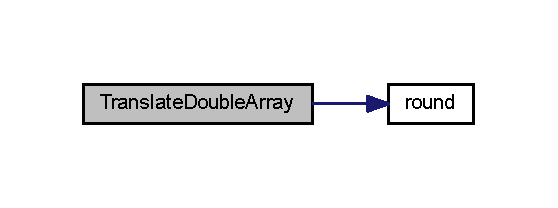
\includegraphics[width=268pt]{doublearray_8cpp_ad38de193265b9dee386ec39996cf8612_cgraph}
\end{center}
\end{figure}


\hypertarget{doublearray_8cpp_a270594add95139649fdc8e84caa67169}{\index{doublearray.\-cpp@{doublearray.\-cpp}!Transpose\-Double\-Array@{Transpose\-Double\-Array}}
\index{Transpose\-Double\-Array@{Transpose\-Double\-Array}!doublearray.cpp@{doublearray.\-cpp}}
\subsubsection[{Transpose\-Double\-Array}]{\setlength{\rightskip}{0pt plus 5cm}void Transpose\-Double\-Array (
\begin{DoxyParamCaption}
\item[{double $\ast$}]{arr, }
\item[{int}]{N1, }
\item[{int}]{N2, }
\item[{double $\ast$\&}]{arr\-Out, }
\item[{int \&}]{M1, }
\item[{int \&}]{M2}
\end{DoxyParamCaption}
)}}\label{doublearray_8cpp_a270594add95139649fdc8e84caa67169}


Definition at line 673 of file doublearray.\-cpp.

\hypertarget{doublearray_8cpp_a18bd2f80b4e24d8ba98fd4ad0601b967}{\index{doublearray.\-cpp@{doublearray.\-cpp}!Zero\-Double\-Array@{Zero\-Double\-Array}}
\index{Zero\-Double\-Array@{Zero\-Double\-Array}!doublearray.cpp@{doublearray.\-cpp}}
\subsubsection[{Zero\-Double\-Array}]{\setlength{\rightskip}{0pt plus 5cm}void Zero\-Double\-Array (
\begin{DoxyParamCaption}
\item[{double $\ast$\&}]{arr, }
\item[{int}]{N1, }
\item[{int}]{N2}
\end{DoxyParamCaption}
)}}\label{doublearray_8cpp_a18bd2f80b4e24d8ba98fd4ad0601b967}


Definition at line 855 of file doublearray.\-cpp.


\hypertarget{edge_8cpp}{\section{build/core/edge.cpp File Reference}
\label{edge_8cpp}\index{build/core/edge.\-cpp@{build/core/edge.\-cpp}}
}
{\ttfamily \#include $<$iostream$>$}\\*
{\ttfamily \#include $<$math.\-h$>$}\\*
{\ttfamily \#include \char`\"{}core/core.\-h\char`\"{}}\\*
Include dependency graph for edge.\-cpp\-:
\nopagebreak
\begin{figure}[H]
\begin{center}
\leavevmode
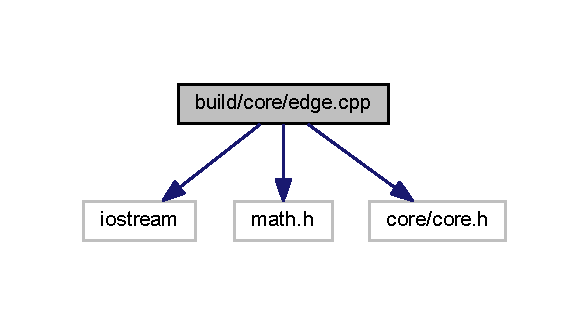
\includegraphics[width=282pt]{edge_8cpp__incl}
\end{center}
\end{figure}
\subsection*{Functions}
\begin{DoxyCompactItemize}
\item 
ostream \& \hyperlink{edge_8cpp_a9f33fecfcff810dd3ad378d382ef02b2}{operator$<$$<$} (ostream \&os, const Edge \&e)
\item 
istream \& \hyperlink{edge_8cpp_ad46346f3781394c9f7ec5d77f60c2522}{operator$>$$>$} (istream \&is, Edge \&e)
\end{DoxyCompactItemize}


\subsection{Function Documentation}
\hypertarget{edge_8cpp_a9f33fecfcff810dd3ad378d382ef02b2}{\index{edge.\-cpp@{edge.\-cpp}!operator$<$$<$@{operator$<$$<$}}
\index{operator$<$$<$@{operator$<$$<$}!edge.cpp@{edge.\-cpp}}
\subsubsection[{operator$<$$<$}]{\setlength{\rightskip}{0pt plus 5cm}ostream\& operator$<$$<$ (
\begin{DoxyParamCaption}
\item[{ostream \&}]{os, }
\item[{const Edge \&}]{e}
\end{DoxyParamCaption}
)}}\label{edge_8cpp_a9f33fecfcff810dd3ad378d382ef02b2}


Definition at line 7 of file edge.\-cpp.

\hypertarget{edge_8cpp_ad46346f3781394c9f7ec5d77f60c2522}{\index{edge.\-cpp@{edge.\-cpp}!operator$>$$>$@{operator$>$$>$}}
\index{operator$>$$>$@{operator$>$$>$}!edge.cpp@{edge.\-cpp}}
\subsubsection[{operator$>$$>$}]{\setlength{\rightskip}{0pt plus 5cm}istream\& operator$>$$>$ (
\begin{DoxyParamCaption}
\item[{istream \&}]{is, }
\item[{Edge \&}]{e}
\end{DoxyParamCaption}
)}}\label{edge_8cpp_ad46346f3781394c9f7ec5d77f60c2522}


Definition at line 17 of file edge.\-cpp.


\hypertarget{ellipse_8cpp}{\section{build/core/ellipse.cpp File Reference}
\label{ellipse_8cpp}\index{build/core/ellipse.\-cpp@{build/core/ellipse.\-cpp}}
}
{\ttfamily \#include \char`\"{}core/core.\-h\char`\"{}}\\*
{\ttfamily \#include $<$math.\-h$>$}\\*
{\ttfamily \#include $<$iostream$>$}\\*
Include dependency graph for ellipse.\-cpp\-:
\nopagebreak
\begin{figure}[H]
\begin{center}
\leavevmode
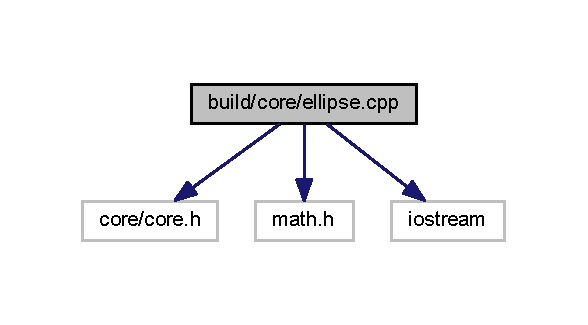
\includegraphics[width=282pt]{ellipse_8cpp__incl}
\end{center}
\end{figure}
\subsection*{Functions}
\begin{DoxyCompactItemize}
\item 
void \hyperlink{ellipse_8cpp_ae494b0e4133b1b8b4eaf339383479221}{Ellipse} (int $\ast$img, int w, int h, double cx, double cy, double rx, double ry, int val)
\item 
void \hyperlink{ellipse_8cpp_a24f9c0ec7b6928b7b615f784a713af69}{Fill\-Ellipse} (int $\ast$img, int w, int h, double cx, double cy, double rx, double ry, int val)
\end{DoxyCompactItemize}


\subsection{Function Documentation}
\hypertarget{ellipse_8cpp_ae494b0e4133b1b8b4eaf339383479221}{\index{ellipse.\-cpp@{ellipse.\-cpp}!Ellipse@{Ellipse}}
\index{Ellipse@{Ellipse}!ellipse.cpp@{ellipse.\-cpp}}
\subsubsection[{Ellipse}]{\setlength{\rightskip}{0pt plus 5cm}void Ellipse (
\begin{DoxyParamCaption}
\item[{int $\ast$}]{img, }
\item[{int}]{w, }
\item[{int}]{h, }
\item[{double}]{cx, }
\item[{double}]{cy, }
\item[{double}]{rx, }
\item[{double}]{ry, }
\item[{int}]{val}
\end{DoxyParamCaption}
)}}\label{ellipse_8cpp_ae494b0e4133b1b8b4eaf339383479221}


Definition at line 7 of file ellipse.\-cpp.



Here is the call graph for this function\-:
\nopagebreak
\begin{figure}[H]
\begin{center}
\leavevmode
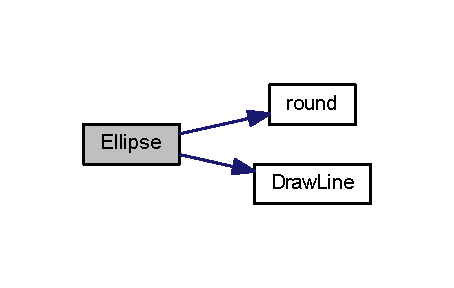
\includegraphics[width=218pt]{ellipse_8cpp_ae494b0e4133b1b8b4eaf339383479221_cgraph}
\end{center}
\end{figure}


\hypertarget{ellipse_8cpp_a24f9c0ec7b6928b7b615f784a713af69}{\index{ellipse.\-cpp@{ellipse.\-cpp}!Fill\-Ellipse@{Fill\-Ellipse}}
\index{Fill\-Ellipse@{Fill\-Ellipse}!ellipse.cpp@{ellipse.\-cpp}}
\subsubsection[{Fill\-Ellipse}]{\setlength{\rightskip}{0pt plus 5cm}void Fill\-Ellipse (
\begin{DoxyParamCaption}
\item[{int $\ast$}]{img, }
\item[{int}]{w, }
\item[{int}]{h, }
\item[{double}]{cx, }
\item[{double}]{cy, }
\item[{double}]{rx, }
\item[{double}]{ry, }
\item[{int}]{val}
\end{DoxyParamCaption}
)}}\label{ellipse_8cpp_a24f9c0ec7b6928b7b615f784a713af69}


Definition at line 27 of file ellipse.\-cpp.


\hypertarget{font_8cpp}{\section{build/core/font.cpp File Reference}
\label{font_8cpp}\index{build/core/font.\-cpp@{build/core/font.\-cpp}}
}
{\ttfamily \#include $<$iostream$>$}\\*
{\ttfamily \#include \char`\"{}core/core.\-h\char`\"{}}\\*
{\ttfamily \#include $<$fstream$>$}\\*
Include dependency graph for font.\-cpp\-:
\nopagebreak
\begin{figure}[H]
\begin{center}
\leavevmode
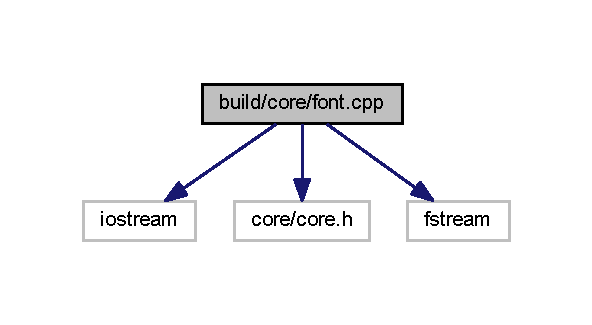
\includegraphics[width=284pt]{font_8cpp__incl}
\end{center}
\end{figure}
\subsection*{Functions}
\begin{DoxyCompactItemize}
\item 
void \hyperlink{font_8cpp_a2492fc8b784f947550b7cf0fda9f62cf}{Put\-Symbol} (int $\ast$img, int N1, int N2, char ch, int x0, int y0, char $\ast$font, int sx, int sy, int color)
\item 
void \hyperlink{font_8cpp_a13f05cf4f10d9e9aa29bb3c41fc8fbbc}{Put\-Symbol\-Transform} (int \&x, int \&y, int sx, int sy)
\item 
void \hyperlink{font_8cpp_a708194f6b8fd011ef16e6730546c5850}{Put\-Text} (int $\ast$img, int N1, int N2, char $\ast$str, int x0, int y0, char $\ast$font, int sx, int sy, double kern, int color)
\end{DoxyCompactItemize}


\subsection{Function Documentation}
\hypertarget{font_8cpp_a2492fc8b784f947550b7cf0fda9f62cf}{\index{font.\-cpp@{font.\-cpp}!Put\-Symbol@{Put\-Symbol}}
\index{Put\-Symbol@{Put\-Symbol}!font.cpp@{font.\-cpp}}
\subsubsection[{Put\-Symbol}]{\setlength{\rightskip}{0pt plus 5cm}void Put\-Symbol (
\begin{DoxyParamCaption}
\item[{int $\ast$}]{img, }
\item[{int}]{N1, }
\item[{int}]{N2, }
\item[{char}]{ch, }
\item[{int}]{x0, }
\item[{int}]{y0, }
\item[{char $\ast$}]{font, }
\item[{int}]{sx, }
\item[{int}]{sy, }
\item[{int}]{color}
\end{DoxyParamCaption}
)}}\label{font_8cpp_a2492fc8b784f947550b7cf0fda9f62cf}


Definition at line 7 of file font.\-cpp.



Here is the call graph for this function\-:
\nopagebreak
\begin{figure}[H]
\begin{center}
\leavevmode
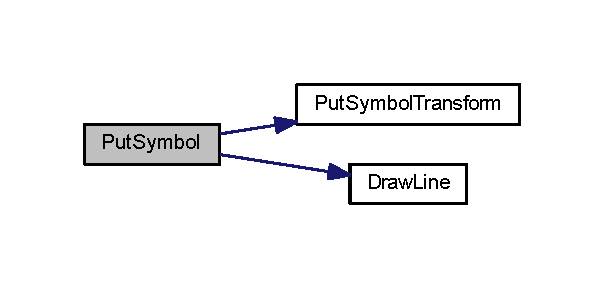
\includegraphics[width=290pt]{font_8cpp_a2492fc8b784f947550b7cf0fda9f62cf_cgraph}
\end{center}
\end{figure}


\hypertarget{font_8cpp_a13f05cf4f10d9e9aa29bb3c41fc8fbbc}{\index{font.\-cpp@{font.\-cpp}!Put\-Symbol\-Transform@{Put\-Symbol\-Transform}}
\index{Put\-Symbol\-Transform@{Put\-Symbol\-Transform}!font.cpp@{font.\-cpp}}
\subsubsection[{Put\-Symbol\-Transform}]{\setlength{\rightskip}{0pt plus 5cm}void Put\-Symbol\-Transform (
\begin{DoxyParamCaption}
\item[{int \&}]{x, }
\item[{int \&}]{y, }
\item[{int}]{sx, }
\item[{int}]{sy}
\end{DoxyParamCaption}
)}}\label{font_8cpp_a13f05cf4f10d9e9aa29bb3c41fc8fbbc}


Definition at line 65 of file font.\-cpp.

\hypertarget{font_8cpp_a708194f6b8fd011ef16e6730546c5850}{\index{font.\-cpp@{font.\-cpp}!Put\-Text@{Put\-Text}}
\index{Put\-Text@{Put\-Text}!font.cpp@{font.\-cpp}}
\subsubsection[{Put\-Text}]{\setlength{\rightskip}{0pt plus 5cm}void Put\-Text (
\begin{DoxyParamCaption}
\item[{int $\ast$}]{img, }
\item[{int}]{N1, }
\item[{int}]{N2, }
\item[{char $\ast$}]{str, }
\item[{int}]{x0, }
\item[{int}]{y0, }
\item[{char $\ast$}]{font, }
\item[{int}]{sx, }
\item[{int}]{sy, }
\item[{double}]{kern, }
\item[{int}]{color}
\end{DoxyParamCaption}
)}}\label{font_8cpp_a708194f6b8fd011ef16e6730546c5850}


Definition at line 74 of file font.\-cpp.



Here is the call graph for this function\-:
\nopagebreak
\begin{figure}[H]
\begin{center}
\leavevmode
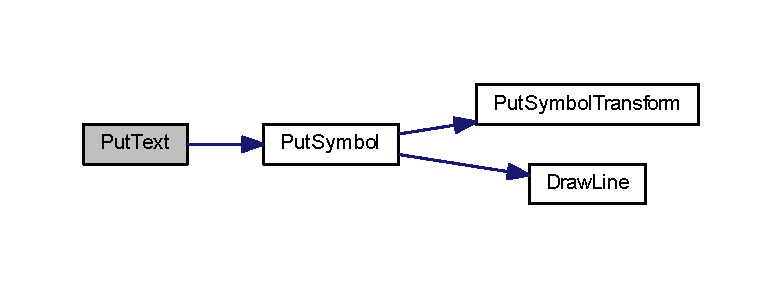
\includegraphics[width=350pt]{font_8cpp_a708194f6b8fd011ef16e6730546c5850_cgraph}
\end{center}
\end{figure}



\hypertarget{graph_8cpp}{\section{build/core/graph.cpp File Reference}
\label{graph_8cpp}\index{build/core/graph.\-cpp@{build/core/graph.\-cpp}}
}
{\ttfamily \#include $<$iostream$>$}\\*
{\ttfamily \#include $<$list$>$}\\*
{\ttfamily \#include $<$string$>$}\\*
{\ttfamily \#include $<$fstream$>$}\\*
{\ttfamily \#include \char`\"{}core/core.\-h\char`\"{}}\\*
Include dependency graph for graph.\-cpp\-:
\nopagebreak
\begin{figure}[H]
\begin{center}
\leavevmode
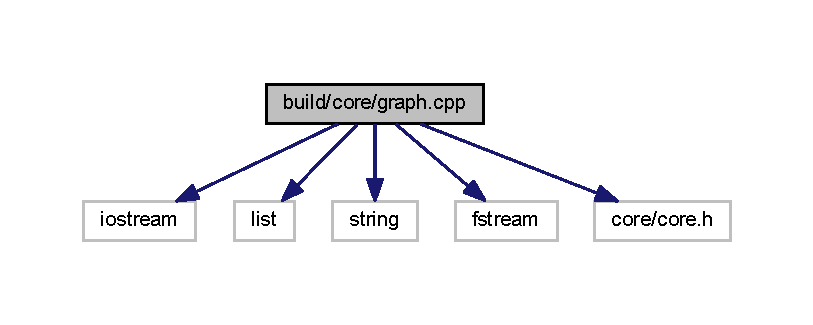
\includegraphics[width=350pt]{graph_8cpp__incl}
\end{center}
\end{figure}

\hypertarget{graph__image_8cpp}{\section{build/core/graph\-\_\-image.cpp File Reference}
\label{graph__image_8cpp}\index{build/core/graph\-\_\-image.\-cpp@{build/core/graph\-\_\-image.\-cpp}}
}
{\ttfamily \#include \char`\"{}core/core.\-h\char`\"{}}\\*
{\ttfamily \#include $<$list$>$}\\*
{\ttfamily \#include $<$math.\-h$>$}\\*
Include dependency graph for graph\-\_\-image.\-cpp\-:
\nopagebreak
\begin{figure}[H]
\begin{center}
\leavevmode
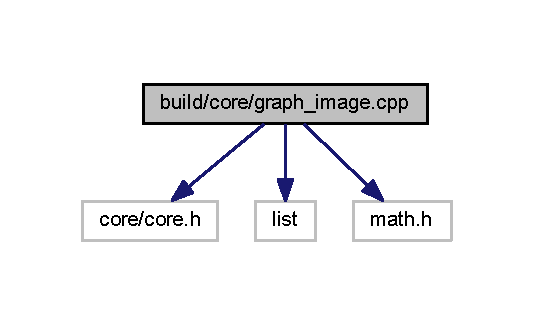
\includegraphics[width=256pt]{graph__image_8cpp__incl}
\end{center}
\end{figure}
\subsection*{Functions}
\begin{DoxyCompactItemize}
\item 
void \hyperlink{graph__image_8cpp_ae036a00a194002b0401a26d4b6bc7227}{Draw\-Graph} (int $\ast$img, int w, int h, Graph $\ast$G, point\-Double $\ast$pts)
\item 
void \hyperlink{graph__image_8cpp_ab203c5b0c23b11d43e9b489fcbf359d3}{Draw\-Arrow} (int $\ast$\&img, int w, int h, double x1, double y1, double x2, double y2, int color, double r, double phi)
\item 
void \hyperlink{graph__image_8cpp_a69b98d60d7e0cef72293ed7f8cdf3bc6}{Draw\-Node} (int $\ast$img, int w, int h, Node v, point\-Double p, double \&r)
\end{DoxyCompactItemize}


\subsection{Function Documentation}
\hypertarget{graph__image_8cpp_ab203c5b0c23b11d43e9b489fcbf359d3}{\index{graph\-\_\-image.\-cpp@{graph\-\_\-image.\-cpp}!Draw\-Arrow@{Draw\-Arrow}}
\index{Draw\-Arrow@{Draw\-Arrow}!graph_image.cpp@{graph\-\_\-image.\-cpp}}
\subsubsection[{Draw\-Arrow}]{\setlength{\rightskip}{0pt plus 5cm}void Draw\-Arrow (
\begin{DoxyParamCaption}
\item[{int $\ast$\&}]{img, }
\item[{int}]{w, }
\item[{int}]{h, }
\item[{double}]{x1, }
\item[{double}]{y1, }
\item[{double}]{x2, }
\item[{double}]{y2, }
\item[{int}]{color, }
\item[{double}]{r, }
\item[{double}]{phi}
\end{DoxyParamCaption}
)}}\label{graph__image_8cpp_ab203c5b0c23b11d43e9b489fcbf359d3}


Definition at line 36 of file graph\-\_\-image.\-cpp.



Here is the call graph for this function\-:
\nopagebreak
\begin{figure}[H]
\begin{center}
\leavevmode
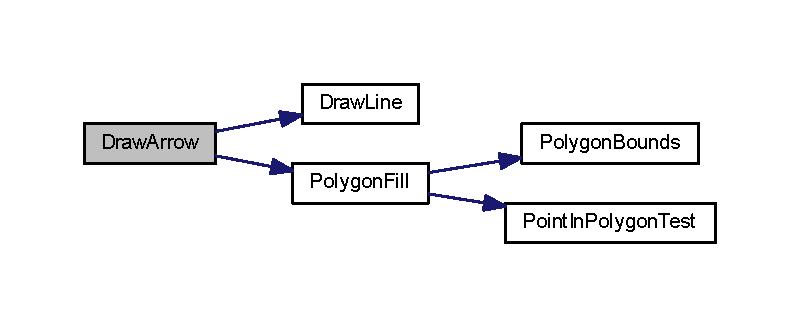
\includegraphics[width=350pt]{graph__image_8cpp_ab203c5b0c23b11d43e9b489fcbf359d3_cgraph}
\end{center}
\end{figure}


\hypertarget{graph__image_8cpp_ae036a00a194002b0401a26d4b6bc7227}{\index{graph\-\_\-image.\-cpp@{graph\-\_\-image.\-cpp}!Draw\-Graph@{Draw\-Graph}}
\index{Draw\-Graph@{Draw\-Graph}!graph_image.cpp@{graph\-\_\-image.\-cpp}}
\subsubsection[{Draw\-Graph}]{\setlength{\rightskip}{0pt plus 5cm}void Draw\-Graph (
\begin{DoxyParamCaption}
\item[{int $\ast$}]{img, }
\item[{int}]{w, }
\item[{int}]{h, }
\item[{Graph $\ast$}]{G, }
\item[{point\-Double $\ast$}]{pts}
\end{DoxyParamCaption}
)}}\label{graph__image_8cpp_ae036a00a194002b0401a26d4b6bc7227}


Definition at line 5 of file graph\-\_\-image.\-cpp.



Here is the call graph for this function\-:
\nopagebreak
\begin{figure}[H]
\begin{center}
\leavevmode
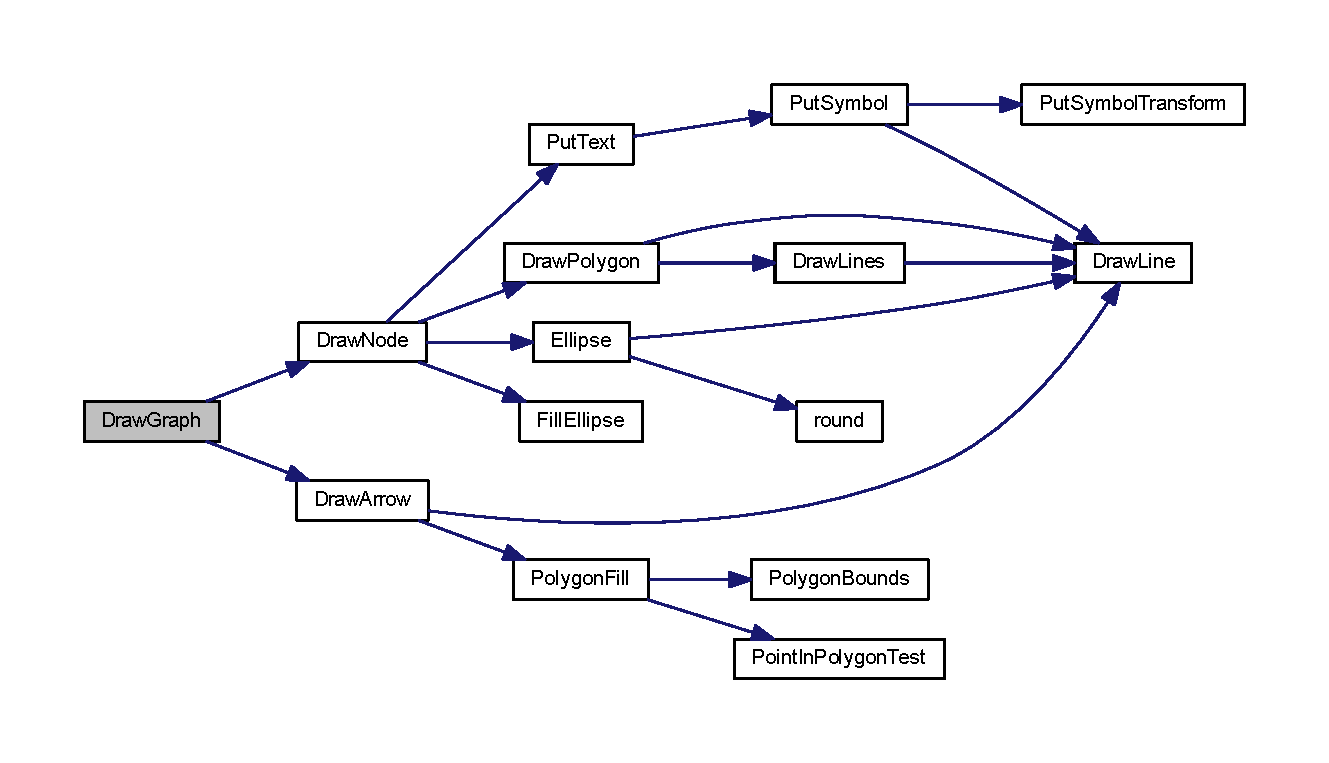
\includegraphics[width=350pt]{graph__image_8cpp_ae036a00a194002b0401a26d4b6bc7227_cgraph}
\end{center}
\end{figure}


\hypertarget{graph__image_8cpp_a69b98d60d7e0cef72293ed7f8cdf3bc6}{\index{graph\-\_\-image.\-cpp@{graph\-\_\-image.\-cpp}!Draw\-Node@{Draw\-Node}}
\index{Draw\-Node@{Draw\-Node}!graph_image.cpp@{graph\-\_\-image.\-cpp}}
\subsubsection[{Draw\-Node}]{\setlength{\rightskip}{0pt plus 5cm}void Draw\-Node (
\begin{DoxyParamCaption}
\item[{int $\ast$}]{img, }
\item[{int}]{w, }
\item[{int}]{h, }
\item[{Node}]{v, }
\item[{point\-Double}]{p, }
\item[{double \&}]{r}
\end{DoxyParamCaption}
)}}\label{graph__image_8cpp_a69b98d60d7e0cef72293ed7f8cdf3bc6}


Definition at line 58 of file graph\-\_\-image.\-cpp.



Here is the call graph for this function\-:
\nopagebreak
\begin{figure}[H]
\begin{center}
\leavevmode
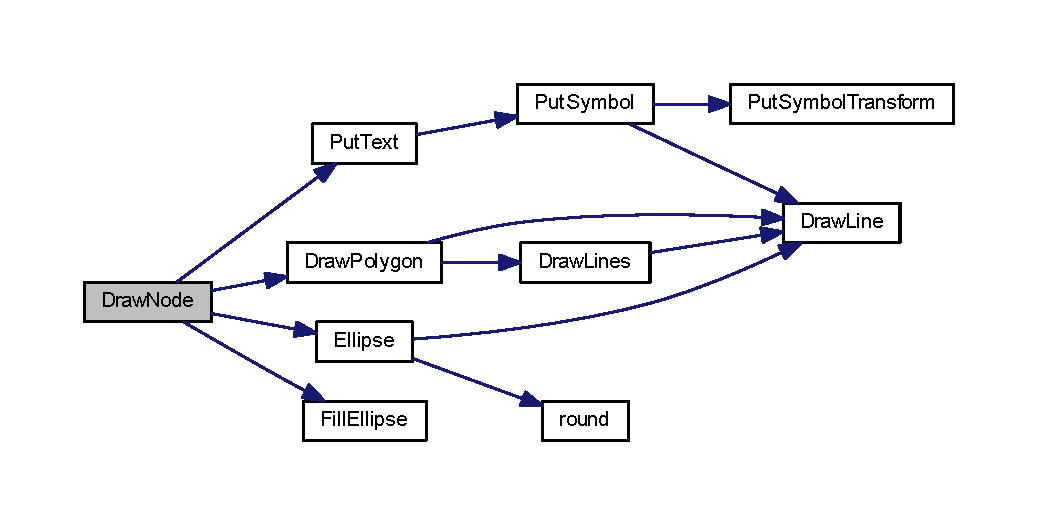
\includegraphics[width=350pt]{graph__image_8cpp_a69b98d60d7e0cef72293ed7f8cdf3bc6_cgraph}
\end{center}
\end{figure}



\hypertarget{int__images_8cpp}{\section{build/core/int\-\_\-images.cpp File Reference}
\label{int__images_8cpp}\index{build/core/int\-\_\-images.\-cpp@{build/core/int\-\_\-images.\-cpp}}
}
{\ttfamily \#include \char`\"{}core/int\-\_\-images.\-h\char`\"{}}\\*
{\ttfamily \#include $<$math.\-h$>$}\\*
Include dependency graph for int\-\_\-images.\-cpp\-:
\nopagebreak
\begin{figure}[H]
\begin{center}
\leavevmode
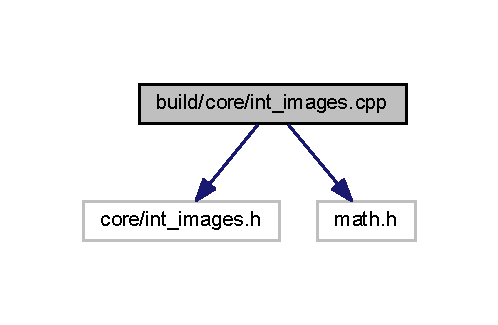
\includegraphics[width=239pt]{int__images_8cpp__incl}
\end{center}
\end{figure}
\subsection*{Functions}
\begin{DoxyCompactItemize}
\item 
void \hyperlink{int__images_8cpp_a568053681a5be2f596275673cc5e1ca8}{Transpose\-Int\-Array} (int $\ast$image, int N1, int N2, int $\ast$\&image\-T, int \&M1, int \&M2)
\item 
void \hyperlink{int__images_8cpp_a9d494ac577b8f730f707bccca450c709}{Set\-Int\-Array} (int $\ast$\&image, int N1, int N2, int val)
\item 
void \hyperlink{int__images_8cpp_a5e71256621170542d1cdf2ad8e4014ae}{Zero\-Int\-Array} (int $\ast$\&image, int N1, int N2)
\item 
void \hyperlink{int__images_8cpp_a3cc4ac0921702a9e1444dec0b1ac6c67}{Copy\-Double\-To\-Int\-Array} (double $\ast$arr, int $\ast$\&image, int N1, int N2)
\item 
void \hyperlink{int__images_8cpp_a52256a9a6fe5c6129391f2314bedf948}{Copy\-Int\-To\-Double\-Array} (int $\ast$image, double $\ast$\&arr, int N1, int N2)
\item 
void \hyperlink{int__images_8cpp_aba51d8e304322c1c4ae2283aca9ea218}{Concat\-Two\-Images\-By\-Width} (int $\ast$image\-A, int $\ast$image\-B, int $\ast$\&image\-Out, int Width\-A, int Width\-B, int Height)
\item 
void \hyperlink{int__images_8cpp_a78fd5c1f36ae8a7e7371412aef1ec4e0}{Convolve\-Int\-Arrays} (int $\ast$image1, int $\ast$image2, int $\ast$\&image3, int N1, int N2, int M1, int M2)
\item 
void \hyperlink{int__images_8cpp_a4bd82ce1c04b38108353551c51211a00}{Correct\-Signed\-Word\-Image} (int $\ast$\&image, int N1, int N2)
\end{DoxyCompactItemize}


\subsection{Function Documentation}
\hypertarget{int__images_8cpp_aba51d8e304322c1c4ae2283aca9ea218}{\index{int\-\_\-images.\-cpp@{int\-\_\-images.\-cpp}!Concat\-Two\-Images\-By\-Width@{Concat\-Two\-Images\-By\-Width}}
\index{Concat\-Two\-Images\-By\-Width@{Concat\-Two\-Images\-By\-Width}!int_images.cpp@{int\-\_\-images.\-cpp}}
\subsubsection[{Concat\-Two\-Images\-By\-Width}]{\setlength{\rightskip}{0pt plus 5cm}void Concat\-Two\-Images\-By\-Width (
\begin{DoxyParamCaption}
\item[{int $\ast$}]{image\-A, }
\item[{int $\ast$}]{image\-B, }
\item[{int $\ast$\&}]{image\-Out, }
\item[{int}]{Width\-A, }
\item[{int}]{Width\-B, }
\item[{int}]{Height}
\end{DoxyParamCaption}
)}}\label{int__images_8cpp_aba51d8e304322c1c4ae2283aca9ea218}


Definition at line 47 of file int\-\_\-images.\-cpp.

\hypertarget{int__images_8cpp_a78fd5c1f36ae8a7e7371412aef1ec4e0}{\index{int\-\_\-images.\-cpp@{int\-\_\-images.\-cpp}!Convolve\-Int\-Arrays@{Convolve\-Int\-Arrays}}
\index{Convolve\-Int\-Arrays@{Convolve\-Int\-Arrays}!int_images.cpp@{int\-\_\-images.\-cpp}}
\subsubsection[{Convolve\-Int\-Arrays}]{\setlength{\rightskip}{0pt plus 5cm}void Convolve\-Int\-Arrays (
\begin{DoxyParamCaption}
\item[{int $\ast$}]{image1, }
\item[{int $\ast$}]{image2, }
\item[{int $\ast$\&}]{image3, }
\item[{int}]{N1, }
\item[{int}]{N2, }
\item[{int}]{M1, }
\item[{int}]{M2}
\end{DoxyParamCaption}
)}}\label{int__images_8cpp_a78fd5c1f36ae8a7e7371412aef1ec4e0}


Definition at line 76 of file int\-\_\-images.\-cpp.

\hypertarget{int__images_8cpp_a3cc4ac0921702a9e1444dec0b1ac6c67}{\index{int\-\_\-images.\-cpp@{int\-\_\-images.\-cpp}!Copy\-Double\-To\-Int\-Array@{Copy\-Double\-To\-Int\-Array}}
\index{Copy\-Double\-To\-Int\-Array@{Copy\-Double\-To\-Int\-Array}!int_images.cpp@{int\-\_\-images.\-cpp}}
\subsubsection[{Copy\-Double\-To\-Int\-Array}]{\setlength{\rightskip}{0pt plus 5cm}void Copy\-Double\-To\-Int\-Array (
\begin{DoxyParamCaption}
\item[{double $\ast$}]{arr, }
\item[{int $\ast$\&}]{image, }
\item[{int}]{N1, }
\item[{int}]{N2}
\end{DoxyParamCaption}
)}}\label{int__images_8cpp_a3cc4ac0921702a9e1444dec0b1ac6c67}


Definition at line 27 of file int\-\_\-images.\-cpp.

\hypertarget{int__images_8cpp_a52256a9a6fe5c6129391f2314bedf948}{\index{int\-\_\-images.\-cpp@{int\-\_\-images.\-cpp}!Copy\-Int\-To\-Double\-Array@{Copy\-Int\-To\-Double\-Array}}
\index{Copy\-Int\-To\-Double\-Array@{Copy\-Int\-To\-Double\-Array}!int_images.cpp@{int\-\_\-images.\-cpp}}
\subsubsection[{Copy\-Int\-To\-Double\-Array}]{\setlength{\rightskip}{0pt plus 5cm}void Copy\-Int\-To\-Double\-Array (
\begin{DoxyParamCaption}
\item[{int $\ast$}]{image, }
\item[{double $\ast$\&}]{arr, }
\item[{int}]{N1, }
\item[{int}]{N2}
\end{DoxyParamCaption}
)}}\label{int__images_8cpp_a52256a9a6fe5c6129391f2314bedf948}


Definition at line 37 of file int\-\_\-images.\-cpp.

\hypertarget{int__images_8cpp_a4bd82ce1c04b38108353551c51211a00}{\index{int\-\_\-images.\-cpp@{int\-\_\-images.\-cpp}!Correct\-Signed\-Word\-Image@{Correct\-Signed\-Word\-Image}}
\index{Correct\-Signed\-Word\-Image@{Correct\-Signed\-Word\-Image}!int_images.cpp@{int\-\_\-images.\-cpp}}
\subsubsection[{Correct\-Signed\-Word\-Image}]{\setlength{\rightskip}{0pt plus 5cm}void Correct\-Signed\-Word\-Image (
\begin{DoxyParamCaption}
\item[{int $\ast$\&}]{image, }
\item[{int}]{N1, }
\item[{int}]{N2}
\end{DoxyParamCaption}
)}}\label{int__images_8cpp_a4bd82ce1c04b38108353551c51211a00}


Definition at line 97 of file int\-\_\-images.\-cpp.

\hypertarget{int__images_8cpp_a9d494ac577b8f730f707bccca450c709}{\index{int\-\_\-images.\-cpp@{int\-\_\-images.\-cpp}!Set\-Int\-Array@{Set\-Int\-Array}}
\index{Set\-Int\-Array@{Set\-Int\-Array}!int_images.cpp@{int\-\_\-images.\-cpp}}
\subsubsection[{Set\-Int\-Array}]{\setlength{\rightskip}{0pt plus 5cm}void Set\-Int\-Array (
\begin{DoxyParamCaption}
\item[{int $\ast$\&}]{image, }
\item[{int}]{N1, }
\item[{int}]{N2, }
\item[{int}]{val}
\end{DoxyParamCaption}
)}}\label{int__images_8cpp_a9d494ac577b8f730f707bccca450c709}


Definition at line 14 of file int\-\_\-images.\-cpp.

\hypertarget{int__images_8cpp_a568053681a5be2f596275673cc5e1ca8}{\index{int\-\_\-images.\-cpp@{int\-\_\-images.\-cpp}!Transpose\-Int\-Array@{Transpose\-Int\-Array}}
\index{Transpose\-Int\-Array@{Transpose\-Int\-Array}!int_images.cpp@{int\-\_\-images.\-cpp}}
\subsubsection[{Transpose\-Int\-Array}]{\setlength{\rightskip}{0pt plus 5cm}void Transpose\-Int\-Array (
\begin{DoxyParamCaption}
\item[{int $\ast$}]{image, }
\item[{int}]{N1, }
\item[{int}]{N2, }
\item[{int $\ast$\&}]{image\-T, }
\item[{int \&}]{M1, }
\item[{int \&}]{M2}
\end{DoxyParamCaption}
)}}\label{int__images_8cpp_a568053681a5be2f596275673cc5e1ca8}


Definition at line 5 of file int\-\_\-images.\-cpp.

\hypertarget{int__images_8cpp_a5e71256621170542d1cdf2ad8e4014ae}{\index{int\-\_\-images.\-cpp@{int\-\_\-images.\-cpp}!Zero\-Int\-Array@{Zero\-Int\-Array}}
\index{Zero\-Int\-Array@{Zero\-Int\-Array}!int_images.cpp@{int\-\_\-images.\-cpp}}
\subsubsection[{Zero\-Int\-Array}]{\setlength{\rightskip}{0pt plus 5cm}void Zero\-Int\-Array (
\begin{DoxyParamCaption}
\item[{int $\ast$\&}]{image, }
\item[{int}]{N1, }
\item[{int}]{N2}
\end{DoxyParamCaption}
)}}\label{int__images_8cpp_a5e71256621170542d1cdf2ad8e4014ae}


Definition at line 22 of file int\-\_\-images.\-cpp.



Here is the call graph for this function\-:
\nopagebreak
\begin{figure}[H]
\begin{center}
\leavevmode
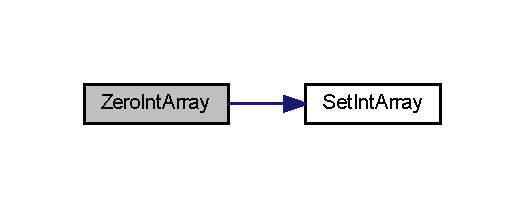
\includegraphics[width=252pt]{int__images_8cpp_a5e71256621170542d1cdf2ad8e4014ae_cgraph}
\end{center}
\end{figure}



\hypertarget{line_8cpp}{\section{build/core/line.cpp File Reference}
\label{line_8cpp}\index{build/core/line.\-cpp@{build/core/line.\-cpp}}
}
{\ttfamily \#include \char`\"{}core/core.\-h\char`\"{}}\\*
{\ttfamily \#include $<$math.\-h$>$}\\*
{\ttfamily \#include $<$iostream$>$}\\*
Include dependency graph for line.\-cpp\-:
\nopagebreak
\begin{figure}[H]
\begin{center}
\leavevmode
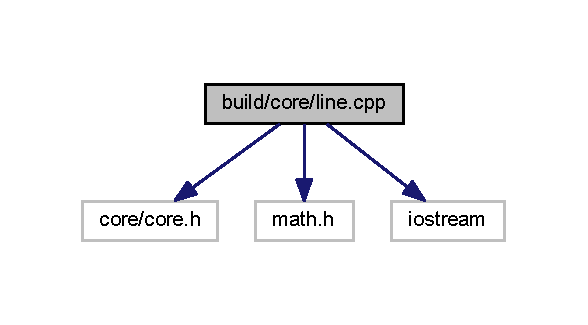
\includegraphics[width=282pt]{line_8cpp__incl}
\end{center}
\end{figure}
\subsection*{Functions}
\begin{DoxyCompactItemize}
\item 
void \hyperlink{line_8cpp_a2dd3334da574f750cad3e1cdc200499b}{Draw\-Line} (Color\-Image img, point p1, point p2, color col)
\item 
void \hyperlink{line_8cpp_a3b772dbfd8b6661761cdc84af64a5786}{Draw\-Line} (int $\ast$\&arr, int N1, int N2, point p1, point p2, int val)
\item 
void \hyperlink{line_8cpp_a1b247393c82acd409e94e15ec3ebf0c6}{Draw\-Line} (int $\ast$\&arr, int N1, int N2, double x1, double y1, double x2, double y2, int val)
\item 
void \hyperlink{line_8cpp_aebb58c3b3fd25a786fa9c580b5614943}{Draw\-Line\-\_\-\-Bresenham} (int $\ast$\&arr, int N1, int N2, double x1, double y1, double x2, double y2, int val)
\end{DoxyCompactItemize}


\subsection{Function Documentation}
\hypertarget{line_8cpp_a2dd3334da574f750cad3e1cdc200499b}{\index{line.\-cpp@{line.\-cpp}!Draw\-Line@{Draw\-Line}}
\index{Draw\-Line@{Draw\-Line}!line.cpp@{line.\-cpp}}
\subsubsection[{Draw\-Line}]{\setlength{\rightskip}{0pt plus 5cm}void Draw\-Line (
\begin{DoxyParamCaption}
\item[{Color\-Image}]{img, }
\item[{point}]{p1, }
\item[{point}]{p2, }
\item[{color}]{col}
\end{DoxyParamCaption}
)}}\label{line_8cpp_a2dd3334da574f750cad3e1cdc200499b}


Definition at line 8 of file line.\-cpp.

\hypertarget{line_8cpp_a3b772dbfd8b6661761cdc84af64a5786}{\index{line.\-cpp@{line.\-cpp}!Draw\-Line@{Draw\-Line}}
\index{Draw\-Line@{Draw\-Line}!line.cpp@{line.\-cpp}}
\subsubsection[{Draw\-Line}]{\setlength{\rightskip}{0pt plus 5cm}void Draw\-Line (
\begin{DoxyParamCaption}
\item[{int $\ast$\&}]{arr, }
\item[{int}]{N1, }
\item[{int}]{N2, }
\item[{point}]{p1, }
\item[{point}]{p2, }
\item[{int}]{val}
\end{DoxyParamCaption}
)}}\label{line_8cpp_a3b772dbfd8b6661761cdc84af64a5786}


Definition at line 17 of file line.\-cpp.



Here is the call graph for this function\-:
\nopagebreak
\begin{figure}[H]
\begin{center}
\leavevmode
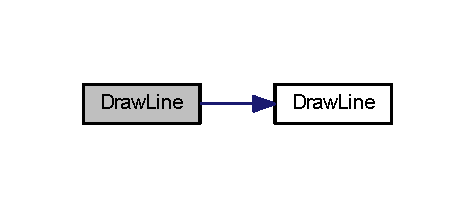
\includegraphics[width=228pt]{line_8cpp_a3b772dbfd8b6661761cdc84af64a5786_cgraph}
\end{center}
\end{figure}


\hypertarget{line_8cpp_a1b247393c82acd409e94e15ec3ebf0c6}{\index{line.\-cpp@{line.\-cpp}!Draw\-Line@{Draw\-Line}}
\index{Draw\-Line@{Draw\-Line}!line.cpp@{line.\-cpp}}
\subsubsection[{Draw\-Line}]{\setlength{\rightskip}{0pt plus 5cm}void Draw\-Line (
\begin{DoxyParamCaption}
\item[{int $\ast$\&}]{arr, }
\item[{int}]{N1, }
\item[{int}]{N2, }
\item[{double}]{x1, }
\item[{double}]{y1, }
\item[{double}]{x2, }
\item[{double}]{y2, }
\item[{int}]{val}
\end{DoxyParamCaption}
)}}\label{line_8cpp_a1b247393c82acd409e94e15ec3ebf0c6}


Definition at line 24 of file line.\-cpp.



Here is the call graph for this function\-:
\nopagebreak
\begin{figure}[H]
\begin{center}
\leavevmode
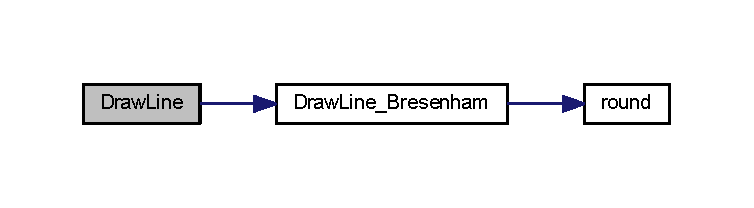
\includegraphics[width=350pt]{line_8cpp_a1b247393c82acd409e94e15ec3ebf0c6_cgraph}
\end{center}
\end{figure}


\hypertarget{line_8cpp_aebb58c3b3fd25a786fa9c580b5614943}{\index{line.\-cpp@{line.\-cpp}!Draw\-Line\-\_\-\-Bresenham@{Draw\-Line\-\_\-\-Bresenham}}
\index{Draw\-Line\-\_\-\-Bresenham@{Draw\-Line\-\_\-\-Bresenham}!line.cpp@{line.\-cpp}}
\subsubsection[{Draw\-Line\-\_\-\-Bresenham}]{\setlength{\rightskip}{0pt plus 5cm}void Draw\-Line\-\_\-\-Bresenham (
\begin{DoxyParamCaption}
\item[{int $\ast$\&}]{arr, }
\item[{int}]{N1, }
\item[{int}]{N2, }
\item[{double}]{x1, }
\item[{double}]{y1, }
\item[{double}]{x2, }
\item[{double}]{y2, }
\item[{int}]{val}
\end{DoxyParamCaption}
)}}\label{line_8cpp_aebb58c3b3fd25a786fa9c580b5614943}


Definition at line 30 of file line.\-cpp.



Here is the call graph for this function\-:
\nopagebreak
\begin{figure}[H]
\begin{center}
\leavevmode
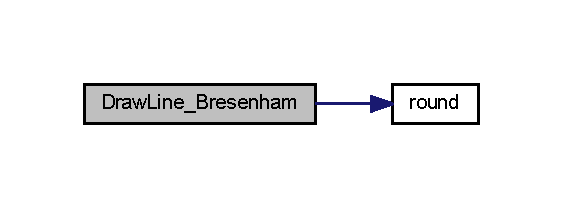
\includegraphics[width=270pt]{line_8cpp_aebb58c3b3fd25a786fa9c580b5614943_cgraph}
\end{center}
\end{figure}



\hypertarget{node_8cpp}{\section{build/core/node.cpp File Reference}
\label{node_8cpp}\index{build/core/node.\-cpp@{build/core/node.\-cpp}}
}
{\ttfamily \#include $<$iostream$>$}\\*
{\ttfamily \#include $<$string$>$}\\*
{\ttfamily \#include $<$math.\-h$>$}\\*
{\ttfamily \#include \char`\"{}core/core.\-h\char`\"{}}\\*
Include dependency graph for node.\-cpp\-:
\nopagebreak
\begin{figure}[H]
\begin{center}
\leavevmode
\includegraphics[width=341pt]{node_8cpp__incl}
\end{center}
\end{figure}
\subsection*{Functions}
\begin{DoxyCompactItemize}
\item 
ostream \& \hyperlink{node_8cpp_ab41a961147c1059c8ae60d0bc1ae3adb}{operator$<$$<$} (ostream \&os, const Node \&v)
\item 
istream \& \hyperlink{node_8cpp_aade4a2cbe6bd4591b0fbce0700e6f8f6}{operator$>$$>$} (istream \&is, Node \&v)
\end{DoxyCompactItemize}


\subsection{Function Documentation}
\hypertarget{node_8cpp_ab41a961147c1059c8ae60d0bc1ae3adb}{\index{node.\-cpp@{node.\-cpp}!operator$<$$<$@{operator$<$$<$}}
\index{operator$<$$<$@{operator$<$$<$}!node.cpp@{node.\-cpp}}
\subsubsection[{operator$<$$<$}]{\setlength{\rightskip}{0pt plus 5cm}ostream\& operator$<$$<$ (
\begin{DoxyParamCaption}
\item[{ostream \&}]{os, }
\item[{const Node \&}]{v}
\end{DoxyParamCaption}
)}}\label{node_8cpp_ab41a961147c1059c8ae60d0bc1ae3adb}


Definition at line 8 of file node.\-cpp.

\hypertarget{node_8cpp_aade4a2cbe6bd4591b0fbce0700e6f8f6}{\index{node.\-cpp@{node.\-cpp}!operator$>$$>$@{operator$>$$>$}}
\index{operator$>$$>$@{operator$>$$>$}!node.cpp@{node.\-cpp}}
\subsubsection[{operator$>$$>$}]{\setlength{\rightskip}{0pt plus 5cm}istream\& operator$>$$>$ (
\begin{DoxyParamCaption}
\item[{istream \&}]{is, }
\item[{Node \&}]{v}
\end{DoxyParamCaption}
)}}\label{node_8cpp_aade4a2cbe6bd4591b0fbce0700e6f8f6}


Definition at line 32 of file node.\-cpp.


\hypertarget{paint_8cpp}{\section{build/core/paint.cpp File Reference}
\label{paint_8cpp}\index{build/core/paint.\-cpp@{build/core/paint.\-cpp}}
}
{\ttfamily \#include \char`\"{}core/core.\-h\char`\"{}}\\*
{\ttfamily \#include $<$deque$>$}\\*
{\ttfamily \#include $<$iostream$>$}\\*
{\ttfamily \#include $<$math.\-h$>$}\\*
Include dependency graph for paint.\-cpp\-:
\nopagebreak
\begin{figure}[H]
\begin{center}
\leavevmode
\includegraphics[width=343pt]{paint_8cpp__incl}
\end{center}
\end{figure}
\subsection*{Functions}
\begin{DoxyCompactItemize}
\item 
void \hyperlink{paint_8cpp_afdc958a7074406769b8fc3ccba93e9f6}{Polygon\-Fill\-Mean} (int $\ast$arr, int N1, int N2, point\-Double $\ast$pp, int N, double val)
\item 
void \hyperlink{paint_8cpp_abb3f588d240c300d2d049660e7064237}{Polygon\-Bounds} (point\-Double $\ast$p, int N, int \&i0, int \&i1, int \&j0, int \&j1)
\item 
void \hyperlink{paint_8cpp_ad69b78615f1146a1e415419f68d21c4e}{Polygon\-Fill} (int $\ast$arr, int N1, int N2, point\-Double $\ast$p, int N, double val)
\item 
void \hyperlink{paint_8cpp_afff8f2a2edda6424b0b602b35a8949bf}{Fill\-Bucket} (int $\ast$\&arr, int N1, int N2, double x, double y, double val, double threshold)
\end{DoxyCompactItemize}


\subsection{Function Documentation}
\hypertarget{paint_8cpp_afff8f2a2edda6424b0b602b35a8949bf}{\index{paint.\-cpp@{paint.\-cpp}!Fill\-Bucket@{Fill\-Bucket}}
\index{Fill\-Bucket@{Fill\-Bucket}!paint.cpp@{paint.\-cpp}}
\subsubsection[{Fill\-Bucket}]{\setlength{\rightskip}{0pt plus 5cm}void Fill\-Bucket (
\begin{DoxyParamCaption}
\item[{int $\ast$\&}]{arr, }
\item[{int}]{N1, }
\item[{int}]{N2, }
\item[{double}]{x, }
\item[{double}]{y, }
\item[{double}]{val, }
\item[{double}]{threshold}
\end{DoxyParamCaption}
)}}\label{paint_8cpp_afff8f2a2edda6424b0b602b35a8949bf}


Definition at line 98 of file paint.\-cpp.



Here is the call graph for this function\-:
\nopagebreak
\begin{figure}[H]
\begin{center}
\leavevmode
\includegraphics[width=256pt]{paint_8cpp_afff8f2a2edda6424b0b602b35a8949bf_cgraph}
\end{center}
\end{figure}


\hypertarget{paint_8cpp_abb3f588d240c300d2d049660e7064237}{\index{paint.\-cpp@{paint.\-cpp}!Polygon\-Bounds@{Polygon\-Bounds}}
\index{Polygon\-Bounds@{Polygon\-Bounds}!paint.cpp@{paint.\-cpp}}
\subsubsection[{Polygon\-Bounds}]{\setlength{\rightskip}{0pt plus 5cm}void Polygon\-Bounds (
\begin{DoxyParamCaption}
\item[{point\-Double $\ast$}]{p, }
\item[{int}]{N, }
\item[{int \&}]{i0, }
\item[{int \&}]{i1, }
\item[{int \&}]{j0, }
\item[{int \&}]{j1}
\end{DoxyParamCaption}
)}}\label{paint_8cpp_abb3f588d240c300d2d049660e7064237}


Definition at line 65 of file paint.\-cpp.

\hypertarget{paint_8cpp_ad69b78615f1146a1e415419f68d21c4e}{\index{paint.\-cpp@{paint.\-cpp}!Polygon\-Fill@{Polygon\-Fill}}
\index{Polygon\-Fill@{Polygon\-Fill}!paint.cpp@{paint.\-cpp}}
\subsubsection[{Polygon\-Fill}]{\setlength{\rightskip}{0pt plus 5cm}void Polygon\-Fill (
\begin{DoxyParamCaption}
\item[{int $\ast$}]{arr, }
\item[{int}]{N1, }
\item[{int}]{N2, }
\item[{point\-Double $\ast$}]{p, }
\item[{int}]{N, }
\item[{double}]{val}
\end{DoxyParamCaption}
)}}\label{paint_8cpp_ad69b78615f1146a1e415419f68d21c4e}


Definition at line 81 of file paint.\-cpp.



Here is the call graph for this function\-:
\nopagebreak
\begin{figure}[H]
\begin{center}
\leavevmode
\includegraphics[width=284pt]{paint_8cpp_ad69b78615f1146a1e415419f68d21c4e_cgraph}
\end{center}
\end{figure}


\hypertarget{paint_8cpp_afdc958a7074406769b8fc3ccba93e9f6}{\index{paint.\-cpp@{paint.\-cpp}!Polygon\-Fill\-Mean@{Polygon\-Fill\-Mean}}
\index{Polygon\-Fill\-Mean@{Polygon\-Fill\-Mean}!paint.cpp@{paint.\-cpp}}
\subsubsection[{Polygon\-Fill\-Mean}]{\setlength{\rightskip}{0pt plus 5cm}void Polygon\-Fill\-Mean (
\begin{DoxyParamCaption}
\item[{int $\ast$}]{arr, }
\item[{int}]{N1, }
\item[{int}]{N2, }
\item[{point\-Double $\ast$}]{pp, }
\item[{int}]{N, }
\item[{double}]{val}
\end{DoxyParamCaption}
)}}\label{paint_8cpp_afdc958a7074406769b8fc3ccba93e9f6}


Definition at line 8 of file paint.\-cpp.



Here is the call graph for this function\-:
\nopagebreak
\begin{figure}[H]
\begin{center}
\leavevmode
\includegraphics[width=308pt]{paint_8cpp_afdc958a7074406769b8fc3ccba93e9f6_cgraph}
\end{center}
\end{figure}



\hypertarget{plot_8cpp}{\section{build/core/plot.cpp File Reference}
\label{plot_8cpp}\index{build/core/plot.\-cpp@{build/core/plot.\-cpp}}
}
{\ttfamily \#include \char`\"{}core/core.\-h\char`\"{}}\\*
{\ttfamily \#include \char`\"{}io/io.\-h\char`\"{}}\\*
{\ttfamily \#include $<$math.\-h$>$}\\*
{\ttfamily \#include $<$iostream$>$}\\*
{\ttfamily \#include $<$fstream$>$}\\*
Include dependency graph for plot.\-cpp\-:
\nopagebreak
\begin{figure}[H]
\begin{center}
\leavevmode
\includegraphics[width=350pt]{plot_8cpp__incl}
\end{center}
\end{figure}
\subsection*{Functions}
\begin{DoxyCompactItemize}
\item 
void \hyperlink{plot_8cpp_ae2a051ac8a896f0274ac928c429bef73}{Plot} (char $\ast$data\-\_\-file, int $\ast$img, int w, int h, int maxval, int x0, int y0, int x1, int y1, bool plot\-\_\-points, bool draw\-\_\-lines, bool draw\-\_\-bars)
\item 
void \hyperlink{plot_8cpp_ac015766db7d2fc6bd12966c73c71fbcb}{Graph\-Paper} (int $\ast$\&img, int w, int h, int maxval, int ni, int nj, int col)
\item 
void \hyperlink{plot_8cpp_ae4572006c82a2c1eed42c7c845e41956}{Graph\-Polygon} (int $\ast$img, int w, int h, int maxval, char $\ast$filename, int xsize, int ysize, int line\-\_\-color, int grid\-\_\-color)
\item 
void \hyperlink{plot_8cpp_a896b061d8c5334d1db327ca0b1f49b71}{Graph\-Polygon2} (int $\ast$img, int w, int h, int maxval, polygon $\ast$ship, int xsize, int ysize, int line\-\_\-color, int grid\-\_\-color)
\end{DoxyCompactItemize}


\subsection{Function Documentation}
\hypertarget{plot_8cpp_ac015766db7d2fc6bd12966c73c71fbcb}{\index{plot.\-cpp@{plot.\-cpp}!Graph\-Paper@{Graph\-Paper}}
\index{Graph\-Paper@{Graph\-Paper}!plot.cpp@{plot.\-cpp}}
\subsubsection[{Graph\-Paper}]{\setlength{\rightskip}{0pt plus 5cm}void Graph\-Paper (
\begin{DoxyParamCaption}
\item[{int $\ast$\&}]{img, }
\item[{int}]{w, }
\item[{int}]{h, }
\item[{int}]{maxval, }
\item[{int}]{ni, }
\item[{int}]{nj, }
\item[{int}]{col}
\end{DoxyParamCaption}
)}}\label{plot_8cpp_ac015766db7d2fc6bd12966c73c71fbcb}


Definition at line 102 of file plot.\-cpp.



Here is the call graph for this function\-:
\nopagebreak
\begin{figure}[H]
\begin{center}
\leavevmode
\includegraphics[width=350pt]{plot_8cpp_ac015766db7d2fc6bd12966c73c71fbcb_cgraph}
\end{center}
\end{figure}


\hypertarget{plot_8cpp_ae4572006c82a2c1eed42c7c845e41956}{\index{plot.\-cpp@{plot.\-cpp}!Graph\-Polygon@{Graph\-Polygon}}
\index{Graph\-Polygon@{Graph\-Polygon}!plot.cpp@{plot.\-cpp}}
\subsubsection[{Graph\-Polygon}]{\setlength{\rightskip}{0pt plus 5cm}void Graph\-Polygon (
\begin{DoxyParamCaption}
\item[{int $\ast$}]{img, }
\item[{int}]{w, }
\item[{int}]{h, }
\item[{int}]{maxval, }
\item[{char $\ast$}]{filename, }
\item[{int}]{xsize, }
\item[{int}]{ysize, }
\item[{int}]{line\-\_\-color, }
\item[{int}]{grid\-\_\-color}
\end{DoxyParamCaption}
)}}\label{plot_8cpp_ae4572006c82a2c1eed42c7c845e41956}


Definition at line 122 of file plot.\-cpp.



Here is the call graph for this function\-:
\nopagebreak
\begin{figure}[H]
\begin{center}
\leavevmode
\includegraphics[width=350pt]{plot_8cpp_ae4572006c82a2c1eed42c7c845e41956_cgraph}
\end{center}
\end{figure}


\hypertarget{plot_8cpp_a896b061d8c5334d1db327ca0b1f49b71}{\index{plot.\-cpp@{plot.\-cpp}!Graph\-Polygon2@{Graph\-Polygon2}}
\index{Graph\-Polygon2@{Graph\-Polygon2}!plot.cpp@{plot.\-cpp}}
\subsubsection[{Graph\-Polygon2}]{\setlength{\rightskip}{0pt plus 5cm}void Graph\-Polygon2 (
\begin{DoxyParamCaption}
\item[{int $\ast$}]{img, }
\item[{int}]{w, }
\item[{int}]{h, }
\item[{int}]{maxval, }
\item[{polygon $\ast$}]{ship, }
\item[{int}]{xsize, }
\item[{int}]{ysize, }
\item[{int}]{line\-\_\-color, }
\item[{int}]{grid\-\_\-color}
\end{DoxyParamCaption}
)}}\label{plot_8cpp_a896b061d8c5334d1db327ca0b1f49b71}


Definition at line 148 of file plot.\-cpp.



Here is the call graph for this function\-:
\nopagebreak
\begin{figure}[H]
\begin{center}
\leavevmode
\includegraphics[width=350pt]{plot_8cpp_a896b061d8c5334d1db327ca0b1f49b71_cgraph}
\end{center}
\end{figure}


\hypertarget{plot_8cpp_ae2a051ac8a896f0274ac928c429bef73}{\index{plot.\-cpp@{plot.\-cpp}!Plot@{Plot}}
\index{Plot@{Plot}!plot.cpp@{plot.\-cpp}}
\subsubsection[{Plot}]{\setlength{\rightskip}{0pt plus 5cm}void Plot (
\begin{DoxyParamCaption}
\item[{char $\ast$}]{data\-\_\-file, }
\item[{int $\ast$}]{img, }
\item[{int}]{w, }
\item[{int}]{h, }
\item[{int}]{maxval, }
\item[{int}]{x0, }
\item[{int}]{y0, }
\item[{int}]{x1, }
\item[{int}]{y1, }
\item[{bool}]{plot\-\_\-points, }
\item[{bool}]{draw\-\_\-lines, }
\item[{bool}]{draw\-\_\-bars}
\end{DoxyParamCaption}
)}}\label{plot_8cpp_ae2a051ac8a896f0274ac928c429bef73}


Definition at line 9 of file plot.\-cpp.



Here is the call graph for this function\-:
\nopagebreak
\begin{figure}[H]
\begin{center}
\leavevmode
\includegraphics[width=350pt]{plot_8cpp_ae2a051ac8a896f0274ac928c429bef73_cgraph}
\end{center}
\end{figure}



\hypertarget{polygon_8cpp}{\section{build/core/polygon.cpp File Reference}
\label{polygon_8cpp}\index{build/core/polygon.\-cpp@{build/core/polygon.\-cpp}}
}
{\ttfamily \#include \char`\"{}core/core.\-h\char`\"{}}\\*
{\ttfamily \#include $<$math.\-h$>$}\\*
{\ttfamily \#include $<$iostream$>$}\\*
Include dependency graph for polygon.\-cpp\-:
\nopagebreak
\begin{figure}[H]
\begin{center}
\leavevmode
\includegraphics[width=282pt]{polygon_8cpp__incl}
\end{center}
\end{figure}
\subsection*{Functions}
\begin{DoxyCompactItemize}
\item 
void \hyperlink{polygon_8cpp_ab0b6a45f2592b9234b25f15c174c080d}{Draw\-Lines} (int $\ast$\&image, int w, int h, point\-Double $\ast$p, int N, int val)
\item 
void \hyperlink{polygon_8cpp_ae435ec75eef851cca7efed6c9fbcee38}{Draw\-Polygon} (int $\ast$\&image, int w, int h, point\-Double $\ast$p, int N, int val)
\item 
int \hyperlink{polygon_8cpp_a10d5ec59ad89effaa33ef1ae3aaf514b}{Point\-In\-Polygon\-Test} (point\-Double $\ast$p, int N, double x, double y)
\item 
double \hyperlink{polygon_8cpp_a65e121aab73f795af35656b884a4f36d}{B\-Spline\-\_\-\-Patch} (double u, double v, double $\ast$P)
\item 
double \hyperlink{polygon_8cpp_a530da8b290fe86dbb356f49b2f8ebe0a}{Bezier\-\_\-\-Patch} (double u, double v, double $\ast$P)
\end{DoxyCompactItemize}


\subsection{Function Documentation}
\hypertarget{polygon_8cpp_a530da8b290fe86dbb356f49b2f8ebe0a}{\index{polygon.\-cpp@{polygon.\-cpp}!Bezier\-\_\-\-Patch@{Bezier\-\_\-\-Patch}}
\index{Bezier\-\_\-\-Patch@{Bezier\-\_\-\-Patch}!polygon.cpp@{polygon.\-cpp}}
\subsubsection[{Bezier\-\_\-\-Patch}]{\setlength{\rightskip}{0pt plus 5cm}double Bezier\-\_\-\-Patch (
\begin{DoxyParamCaption}
\item[{double}]{u, }
\item[{double}]{v, }
\item[{double $\ast$}]{P}
\end{DoxyParamCaption}
)}}\label{polygon_8cpp_a530da8b290fe86dbb356f49b2f8ebe0a}


Definition at line 94 of file polygon.\-cpp.



Here is the call graph for this function\-:
\nopagebreak
\begin{figure}[H]
\begin{center}
\leavevmode
\includegraphics[width=302pt]{polygon_8cpp_a530da8b290fe86dbb356f49b2f8ebe0a_cgraph}
\end{center}
\end{figure}


\hypertarget{polygon_8cpp_a65e121aab73f795af35656b884a4f36d}{\index{polygon.\-cpp@{polygon.\-cpp}!B\-Spline\-\_\-\-Patch@{B\-Spline\-\_\-\-Patch}}
\index{B\-Spline\-\_\-\-Patch@{B\-Spline\-\_\-\-Patch}!polygon.cpp@{polygon.\-cpp}}
\subsubsection[{B\-Spline\-\_\-\-Patch}]{\setlength{\rightskip}{0pt plus 5cm}double B\-Spline\-\_\-\-Patch (
\begin{DoxyParamCaption}
\item[{double}]{u, }
\item[{double}]{v, }
\item[{double $\ast$}]{P}
\end{DoxyParamCaption}
)}}\label{polygon_8cpp_a65e121aab73f795af35656b884a4f36d}


Definition at line 45 of file polygon.\-cpp.



Here is the call graph for this function\-:
\nopagebreak
\begin{figure}[H]
\begin{center}
\leavevmode
\includegraphics[width=308pt]{polygon_8cpp_a65e121aab73f795af35656b884a4f36d_cgraph}
\end{center}
\end{figure}


\hypertarget{polygon_8cpp_ab0b6a45f2592b9234b25f15c174c080d}{\index{polygon.\-cpp@{polygon.\-cpp}!Draw\-Lines@{Draw\-Lines}}
\index{Draw\-Lines@{Draw\-Lines}!polygon.cpp@{polygon.\-cpp}}
\subsubsection[{Draw\-Lines}]{\setlength{\rightskip}{0pt plus 5cm}void Draw\-Lines (
\begin{DoxyParamCaption}
\item[{int $\ast$\&}]{image, }
\item[{int}]{w, }
\item[{int}]{h, }
\item[{point\-Double $\ast$}]{p, }
\item[{int}]{N, }
\item[{int}]{val}
\end{DoxyParamCaption}
)}}\label{polygon_8cpp_ab0b6a45f2592b9234b25f15c174c080d}


Definition at line 7 of file polygon.\-cpp.



Here is the call graph for this function\-:
\nopagebreak
\begin{figure}[H]
\begin{center}
\leavevmode
\includegraphics[width=234pt]{polygon_8cpp_ab0b6a45f2592b9234b25f15c174c080d_cgraph}
\end{center}
\end{figure}


\hypertarget{polygon_8cpp_ae435ec75eef851cca7efed6c9fbcee38}{\index{polygon.\-cpp@{polygon.\-cpp}!Draw\-Polygon@{Draw\-Polygon}}
\index{Draw\-Polygon@{Draw\-Polygon}!polygon.cpp@{polygon.\-cpp}}
\subsubsection[{Draw\-Polygon}]{\setlength{\rightskip}{0pt plus 5cm}void Draw\-Polygon (
\begin{DoxyParamCaption}
\item[{int $\ast$\&}]{image, }
\item[{int}]{w, }
\item[{int}]{h, }
\item[{point\-Double $\ast$}]{p, }
\item[{int}]{N, }
\item[{int}]{val}
\end{DoxyParamCaption}
)}}\label{polygon_8cpp_ae435ec75eef851cca7efed6c9fbcee38}


Definition at line 17 of file polygon.\-cpp.



Here is the call graph for this function\-:
\nopagebreak
\begin{figure}[H]
\begin{center}
\leavevmode
\includegraphics[width=344pt]{polygon_8cpp_ae435ec75eef851cca7efed6c9fbcee38_cgraph}
\end{center}
\end{figure}


\hypertarget{polygon_8cpp_a10d5ec59ad89effaa33ef1ae3aaf514b}{\index{polygon.\-cpp@{polygon.\-cpp}!Point\-In\-Polygon\-Test@{Point\-In\-Polygon\-Test}}
\index{Point\-In\-Polygon\-Test@{Point\-In\-Polygon\-Test}!polygon.cpp@{polygon.\-cpp}}
\subsubsection[{Point\-In\-Polygon\-Test}]{\setlength{\rightskip}{0pt plus 5cm}int Point\-In\-Polygon\-Test (
\begin{DoxyParamCaption}
\item[{point\-Double $\ast$}]{p, }
\item[{int}]{N, }
\item[{double}]{x, }
\item[{double}]{y}
\end{DoxyParamCaption}
)}}\label{polygon_8cpp_a10d5ec59ad89effaa33ef1ae3aaf514b}


Definition at line 29 of file polygon.\-cpp.


\hypertarget{usr__misc_8cpp}{\section{build/core/usr\-\_\-misc.cpp File Reference}
\label{usr__misc_8cpp}\index{build/core/usr\-\_\-misc.\-cpp@{build/core/usr\-\_\-misc.\-cpp}}
}
{\ttfamily \#include \char`\"{}core/usr\-\_\-misc.\-h\char`\"{}}\\*
{\ttfamily \#include $<$iostream$>$}\\*
{\ttfamily \#include $<$math.\-h$>$}\\*
Include dependency graph for usr\-\_\-misc.\-cpp\-:
\nopagebreak
\begin{figure}[H]
\begin{center}
\leavevmode
\includegraphics[width=303pt]{usr__misc_8cpp__incl}
\end{center}
\end{figure}
\subsection*{Functions}
\begin{DoxyCompactItemize}
\item 
char $\ast$ \hyperlink{usr__misc_8cpp_a7a621f07d1f3d8efab05dbb3721d0184}{String\-To\-Uppercase} (char $\ast$\&str)
\item 
void \hyperlink{usr__misc_8cpp_abd9af5ff430750a645fffb17208a8733}{Correct\-Signed\-Byte\-Image} (int $\ast$\&image, int N1, int N2)
\item 
bool \hyperlink{usr__misc_8cpp_aa73bc4e41ee4072e934e2f4635d074f4}{Array\-\_\-\-Support} (int N1, int N2, int x, int y)
\item 
void \hyperlink{usr__misc_8cpp_a1369905afee62639dc2ed307f2f41a1e}{False\-Color} (double t, double mid, int \&r, int \&g, int \&b)
\item 
double \hyperlink{usr__misc_8cpp_a7d54bc171b23d92b6c7ea822c95667df}{Fleck\-\_\-\-L} (double x)
\item 
int \hyperlink{usr__misc_8cpp_a35abf8e6bc22bc3736fbd65416d8c3a2}{round} (double x)
\item 
void \hyperlink{usr__misc_8cpp_a489d747d9f8c2c44426a138df483d6b3}{swap} (double x, double y)
\item 
double \hyperlink{usr__misc_8cpp_a99d386c61332efa7305d0ec6cbb818fe}{My\-\_\-atan2} (double x, double y)
\end{DoxyCompactItemize}


\subsection{Function Documentation}
\hypertarget{usr__misc_8cpp_aa73bc4e41ee4072e934e2f4635d074f4}{\index{usr\-\_\-misc.\-cpp@{usr\-\_\-misc.\-cpp}!Array\-\_\-\-Support@{Array\-\_\-\-Support}}
\index{Array\-\_\-\-Support@{Array\-\_\-\-Support}!usr_misc.cpp@{usr\-\_\-misc.\-cpp}}
\subsubsection[{Array\-\_\-\-Support}]{\setlength{\rightskip}{0pt plus 5cm}bool Array\-\_\-\-Support (
\begin{DoxyParamCaption}
\item[{int}]{N1, }
\item[{int}]{N2, }
\item[{int}]{x, }
\item[{int}]{y}
\end{DoxyParamCaption}
)}}\label{usr__misc_8cpp_aa73bc4e41ee4072e934e2f4635d074f4}


Definition at line 37 of file usr\-\_\-misc.\-cpp.

\hypertarget{usr__misc_8cpp_abd9af5ff430750a645fffb17208a8733}{\index{usr\-\_\-misc.\-cpp@{usr\-\_\-misc.\-cpp}!Correct\-Signed\-Byte\-Image@{Correct\-Signed\-Byte\-Image}}
\index{Correct\-Signed\-Byte\-Image@{Correct\-Signed\-Byte\-Image}!usr_misc.cpp@{usr\-\_\-misc.\-cpp}}
\subsubsection[{Correct\-Signed\-Byte\-Image}]{\setlength{\rightskip}{0pt plus 5cm}void Correct\-Signed\-Byte\-Image (
\begin{DoxyParamCaption}
\item[{int $\ast$\&}]{image, }
\item[{int}]{N1, }
\item[{int}]{N2}
\end{DoxyParamCaption}
)}}\label{usr__misc_8cpp_abd9af5ff430750a645fffb17208a8733}


Definition at line 23 of file usr\-\_\-misc.\-cpp.

\hypertarget{usr__misc_8cpp_a1369905afee62639dc2ed307f2f41a1e}{\index{usr\-\_\-misc.\-cpp@{usr\-\_\-misc.\-cpp}!False\-Color@{False\-Color}}
\index{False\-Color@{False\-Color}!usr_misc.cpp@{usr\-\_\-misc.\-cpp}}
\subsubsection[{False\-Color}]{\setlength{\rightskip}{0pt plus 5cm}void False\-Color (
\begin{DoxyParamCaption}
\item[{double}]{t, }
\item[{double}]{mid, }
\item[{int \&}]{r, }
\item[{int \&}]{g, }
\item[{int \&}]{b}
\end{DoxyParamCaption}
)}}\label{usr__misc_8cpp_a1369905afee62639dc2ed307f2f41a1e}


Definition at line 42 of file usr\-\_\-misc.\-cpp.



Here is the call graph for this function\-:
\nopagebreak
\begin{figure}[H]
\begin{center}
\leavevmode
\includegraphics[width=222pt]{usr__misc_8cpp_a1369905afee62639dc2ed307f2f41a1e_cgraph}
\end{center}
\end{figure}


\hypertarget{usr__misc_8cpp_a7d54bc171b23d92b6c7ea822c95667df}{\index{usr\-\_\-misc.\-cpp@{usr\-\_\-misc.\-cpp}!Fleck\-\_\-\-L@{Fleck\-\_\-\-L}}
\index{Fleck\-\_\-\-L@{Fleck\-\_\-\-L}!usr_misc.cpp@{usr\-\_\-misc.\-cpp}}
\subsubsection[{Fleck\-\_\-\-L}]{\setlength{\rightskip}{0pt plus 5cm}double Fleck\-\_\-\-L (
\begin{DoxyParamCaption}
\item[{double}]{x}
\end{DoxyParamCaption}
)}}\label{usr__misc_8cpp_a7d54bc171b23d92b6c7ea822c95667df}


Definition at line 56 of file usr\-\_\-misc.\-cpp.

\hypertarget{usr__misc_8cpp_a99d386c61332efa7305d0ec6cbb818fe}{\index{usr\-\_\-misc.\-cpp@{usr\-\_\-misc.\-cpp}!My\-\_\-atan2@{My\-\_\-atan2}}
\index{My\-\_\-atan2@{My\-\_\-atan2}!usr_misc.cpp@{usr\-\_\-misc.\-cpp}}
\subsubsection[{My\-\_\-atan2}]{\setlength{\rightskip}{0pt plus 5cm}double My\-\_\-atan2 (
\begin{DoxyParamCaption}
\item[{double}]{x, }
\item[{double}]{y}
\end{DoxyParamCaption}
)}}\label{usr__misc_8cpp_a99d386c61332efa7305d0ec6cbb818fe}


Definition at line 78 of file usr\-\_\-misc.\-cpp.

\hypertarget{usr__misc_8cpp_a35abf8e6bc22bc3736fbd65416d8c3a2}{\index{usr\-\_\-misc.\-cpp@{usr\-\_\-misc.\-cpp}!round@{round}}
\index{round@{round}!usr_misc.cpp@{usr\-\_\-misc.\-cpp}}
\subsubsection[{round}]{\setlength{\rightskip}{0pt plus 5cm}int round (
\begin{DoxyParamCaption}
\item[{double}]{x}
\end{DoxyParamCaption}
)}}\label{usr__misc_8cpp_a35abf8e6bc22bc3736fbd65416d8c3a2}


Definition at line 62 of file usr\-\_\-misc.\-cpp.

\hypertarget{usr__misc_8cpp_a7a621f07d1f3d8efab05dbb3721d0184}{\index{usr\-\_\-misc.\-cpp@{usr\-\_\-misc.\-cpp}!String\-To\-Uppercase@{String\-To\-Uppercase}}
\index{String\-To\-Uppercase@{String\-To\-Uppercase}!usr_misc.cpp@{usr\-\_\-misc.\-cpp}}
\subsubsection[{String\-To\-Uppercase}]{\setlength{\rightskip}{0pt plus 5cm}char$\ast$ String\-To\-Uppercase (
\begin{DoxyParamCaption}
\item[{char $\ast$\&}]{str}
\end{DoxyParamCaption}
)}}\label{usr__misc_8cpp_a7a621f07d1f3d8efab05dbb3721d0184}


Definition at line 8 of file usr\-\_\-misc.\-cpp.

\hypertarget{usr__misc_8cpp_a489d747d9f8c2c44426a138df483d6b3}{\index{usr\-\_\-misc.\-cpp@{usr\-\_\-misc.\-cpp}!swap@{swap}}
\index{swap@{swap}!usr_misc.cpp@{usr\-\_\-misc.\-cpp}}
\subsubsection[{swap}]{\setlength{\rightskip}{0pt plus 5cm}void swap (
\begin{DoxyParamCaption}
\item[{double}]{x, }
\item[{double}]{y}
\end{DoxyParamCaption}
)}}\label{usr__misc_8cpp_a489d747d9f8c2c44426a138df483d6b3}


Definition at line 70 of file usr\-\_\-misc.\-cpp.


\hypertarget{vector3d_8cpp}{\section{build/core/vector3d.cpp File Reference}
\label{vector3d_8cpp}\index{build/core/vector3d.\-cpp@{build/core/vector3d.\-cpp}}
}
{\ttfamily \#include \char`\"{}core/vector3d.\-h\char`\"{}}\\*
{\ttfamily \#include $<$math.\-h$>$}\\*
Include dependency graph for vector3d.\-cpp\-:
\nopagebreak
\begin{figure}[H]
\begin{center}
\leavevmode
\includegraphics[width=227pt]{vector3d_8cpp__incl}
\end{center}
\end{figure}
\subsection*{Functions}
\begin{DoxyCompactItemize}
\item 
float \hyperlink{vector3d_8cpp_a2061ae8a36a2314ae3cbeddbb6ac0519}{Vector\-Magnitude} (Vector3\-D v)
\item 
Vector3\-D \hyperlink{vector3d_8cpp_a73d7c68574f2d8f2076479421647a11c}{Vector\-Normalize} (Vector3\-D v)
\item 
Vector3\-D \hyperlink{vector3d_8cpp_a4b770b50cd06db670fdc0c83c503db86}{Vector\-Add} (Vector3\-D v0, Vector3\-D v1)
\item 
Vector3\-D \hyperlink{vector3d_8cpp_a84d0501de8ca4f3dbffec38bee52f79e}{Vector\-Subtract} (Vector3\-D v0, Vector3\-D v1)
\item 
Vector3\-D \hyperlink{vector3d_8cpp_ace29c7fc5ffc0c37128928cb8543f05a}{Vector\-Scalar\-Mult} (Vector3\-D v0, float scalar)
\item 
Vector3\-D \hyperlink{vector3d_8cpp_a1304cda210f06ace89c97020cb0272ee}{Vector\-Cross} (Vector3\-D v0, Vector3\-D v1)
\item 
float \hyperlink{vector3d_8cpp_aed68e6e81215b24ddab95986b5340fa7}{Vector\-Dot} (Vector3\-D v0, Vector3\-D v1)
\end{DoxyCompactItemize}


\subsection{Function Documentation}
\hypertarget{vector3d_8cpp_a4b770b50cd06db670fdc0c83c503db86}{\index{vector3d.\-cpp@{vector3d.\-cpp}!Vector\-Add@{Vector\-Add}}
\index{Vector\-Add@{Vector\-Add}!vector3d.cpp@{vector3d.\-cpp}}
\subsubsection[{Vector\-Add}]{\setlength{\rightskip}{0pt plus 5cm}Vector3\-D Vector\-Add (
\begin{DoxyParamCaption}
\item[{Vector3\-D}]{v0, }
\item[{Vector3\-D}]{v1}
\end{DoxyParamCaption}
)}}\label{vector3d_8cpp_a4b770b50cd06db670fdc0c83c503db86}


Definition at line 23 of file vector3d.\-cpp.

\hypertarget{vector3d_8cpp_a1304cda210f06ace89c97020cb0272ee}{\index{vector3d.\-cpp@{vector3d.\-cpp}!Vector\-Cross@{Vector\-Cross}}
\index{Vector\-Cross@{Vector\-Cross}!vector3d.cpp@{vector3d.\-cpp}}
\subsubsection[{Vector\-Cross}]{\setlength{\rightskip}{0pt plus 5cm}Vector3\-D Vector\-Cross (
\begin{DoxyParamCaption}
\item[{Vector3\-D}]{v0, }
\item[{Vector3\-D}]{v1}
\end{DoxyParamCaption}
)}}\label{vector3d_8cpp_a1304cda210f06ace89c97020cb0272ee}


Definition at line 48 of file vector3d.\-cpp.

\hypertarget{vector3d_8cpp_aed68e6e81215b24ddab95986b5340fa7}{\index{vector3d.\-cpp@{vector3d.\-cpp}!Vector\-Dot@{Vector\-Dot}}
\index{Vector\-Dot@{Vector\-Dot}!vector3d.cpp@{vector3d.\-cpp}}
\subsubsection[{Vector\-Dot}]{\setlength{\rightskip}{0pt plus 5cm}float Vector\-Dot (
\begin{DoxyParamCaption}
\item[{Vector3\-D}]{v0, }
\item[{Vector3\-D}]{v1}
\end{DoxyParamCaption}
)}}\label{vector3d_8cpp_aed68e6e81215b24ddab95986b5340fa7}


Definition at line 58 of file vector3d.\-cpp.

\hypertarget{vector3d_8cpp_a2061ae8a36a2314ae3cbeddbb6ac0519}{\index{vector3d.\-cpp@{vector3d.\-cpp}!Vector\-Magnitude@{Vector\-Magnitude}}
\index{Vector\-Magnitude@{Vector\-Magnitude}!vector3d.cpp@{vector3d.\-cpp}}
\subsubsection[{Vector\-Magnitude}]{\setlength{\rightskip}{0pt plus 5cm}float Vector\-Magnitude (
\begin{DoxyParamCaption}
\item[{Vector3\-D}]{v}
\end{DoxyParamCaption}
)}}\label{vector3d_8cpp_a2061ae8a36a2314ae3cbeddbb6ac0519}


Definition at line 5 of file vector3d.\-cpp.

\hypertarget{vector3d_8cpp_a73d7c68574f2d8f2076479421647a11c}{\index{vector3d.\-cpp@{vector3d.\-cpp}!Vector\-Normalize@{Vector\-Normalize}}
\index{Vector\-Normalize@{Vector\-Normalize}!vector3d.cpp@{vector3d.\-cpp}}
\subsubsection[{Vector\-Normalize}]{\setlength{\rightskip}{0pt plus 5cm}Vector3\-D Vector\-Normalize (
\begin{DoxyParamCaption}
\item[{Vector3\-D}]{v}
\end{DoxyParamCaption}
)}}\label{vector3d_8cpp_a73d7c68574f2d8f2076479421647a11c}


Definition at line 13 of file vector3d.\-cpp.



Here is the call graph for this function\-:
\nopagebreak
\begin{figure}[H]
\begin{center}
\leavevmode
\includegraphics[width=298pt]{vector3d_8cpp_a73d7c68574f2d8f2076479421647a11c_cgraph}
\end{center}
\end{figure}


\hypertarget{vector3d_8cpp_ace29c7fc5ffc0c37128928cb8543f05a}{\index{vector3d.\-cpp@{vector3d.\-cpp}!Vector\-Scalar\-Mult@{Vector\-Scalar\-Mult}}
\index{Vector\-Scalar\-Mult@{Vector\-Scalar\-Mult}!vector3d.cpp@{vector3d.\-cpp}}
\subsubsection[{Vector\-Scalar\-Mult}]{\setlength{\rightskip}{0pt plus 5cm}Vector3\-D Vector\-Scalar\-Mult (
\begin{DoxyParamCaption}
\item[{Vector3\-D}]{v0, }
\item[{float}]{scalar}
\end{DoxyParamCaption}
)}}\label{vector3d_8cpp_ace29c7fc5ffc0c37128928cb8543f05a}


Definition at line 39 of file vector3d.\-cpp.

\hypertarget{vector3d_8cpp_a84d0501de8ca4f3dbffec38bee52f79e}{\index{vector3d.\-cpp@{vector3d.\-cpp}!Vector\-Subtract@{Vector\-Subtract}}
\index{Vector\-Subtract@{Vector\-Subtract}!vector3d.cpp@{vector3d.\-cpp}}
\subsubsection[{Vector\-Subtract}]{\setlength{\rightskip}{0pt plus 5cm}Vector3\-D Vector\-Subtract (
\begin{DoxyParamCaption}
\item[{Vector3\-D}]{v0, }
\item[{Vector3\-D}]{v1}
\end{DoxyParamCaption}
)}}\label{vector3d_8cpp_a84d0501de8ca4f3dbffec38bee52f79e}


Definition at line 31 of file vector3d.\-cpp.


\hypertarget{dcm_8cpp}{\section{build/io/dcm.cpp File Reference}
\label{dcm_8cpp}\index{build/io/dcm.\-cpp@{build/io/dcm.\-cpp}}
}
{\ttfamily \#include \char`\"{}core/common.\-h\char`\"{}}\\*
{\ttfamily \#include \char`\"{}io/ppm.\-h\char`\"{}}\\*
{\ttfamily \#include $<$iostream$>$}\\*
Include dependency graph for dcm.\-cpp\-:
\nopagebreak
\begin{figure}[H]
\begin{center}
\leavevmode
\includegraphics[width=308pt]{dcm_8cpp__incl}
\end{center}
\end{figure}
\subsection*{Functions}
\begin{DoxyCompactItemize}
\item 
void \hyperlink{dcm_8cpp_aa58e827407ce18e08c71fd5e43cf61e6}{Read\-\_\-\-D\-C\-M\-\_\-\-File} (char $\ast$filename, int \&M\-A\-X\-V\-A\-L, int \&N1, int \&N2, int $\ast$\&image)
\item 
void \hyperlink{dcm_8cpp_a0582d277cff91406840dde5599551afc}{Read\-\_\-\-D\-C\-M\-\_\-\-File\-\_\-\-Info} (char $\ast$filename)
\item 
void \hyperlink{dcm_8cpp_a6466282d9e9771634889a6e4079576a5}{Read\-\_\-\-D\-C\-M\-\_\-\-Options\-\_\-\-File} (char $\ast$filename, char $\ast$options, int \&M\-A\-X\-V\-A\-L, int \&N1, int \&N2, int $\ast$\&image)
\end{DoxyCompactItemize}


\subsection{Function Documentation}
\hypertarget{dcm_8cpp_aa58e827407ce18e08c71fd5e43cf61e6}{\index{dcm.\-cpp@{dcm.\-cpp}!Read\-\_\-\-D\-C\-M\-\_\-\-File@{Read\-\_\-\-D\-C\-M\-\_\-\-File}}
\index{Read\-\_\-\-D\-C\-M\-\_\-\-File@{Read\-\_\-\-D\-C\-M\-\_\-\-File}!dcm.cpp@{dcm.\-cpp}}
\subsubsection[{Read\-\_\-\-D\-C\-M\-\_\-\-File}]{\setlength{\rightskip}{0pt plus 5cm}void Read\-\_\-\-D\-C\-M\-\_\-\-File (
\begin{DoxyParamCaption}
\item[{char $\ast$}]{filename, }
\item[{int \&}]{M\-A\-X\-V\-A\-L, }
\item[{int \&}]{N1, }
\item[{int \&}]{N2, }
\item[{int $\ast$\&}]{image}
\end{DoxyParamCaption}
)}}\label{dcm_8cpp_aa58e827407ce18e08c71fd5e43cf61e6}


Definition at line 8 of file dcm.\-cpp.



Here is the call graph for this function\-:
\nopagebreak
\begin{figure}[H]
\begin{center}
\leavevmode
\includegraphics[width=350pt]{dcm_8cpp_aa58e827407ce18e08c71fd5e43cf61e6_cgraph}
\end{center}
\end{figure}


\hypertarget{dcm_8cpp_a0582d277cff91406840dde5599551afc}{\index{dcm.\-cpp@{dcm.\-cpp}!Read\-\_\-\-D\-C\-M\-\_\-\-File\-\_\-\-Info@{Read\-\_\-\-D\-C\-M\-\_\-\-File\-\_\-\-Info}}
\index{Read\-\_\-\-D\-C\-M\-\_\-\-File\-\_\-\-Info@{Read\-\_\-\-D\-C\-M\-\_\-\-File\-\_\-\-Info}!dcm.cpp@{dcm.\-cpp}}
\subsubsection[{Read\-\_\-\-D\-C\-M\-\_\-\-File\-\_\-\-Info}]{\setlength{\rightskip}{0pt plus 5cm}void Read\-\_\-\-D\-C\-M\-\_\-\-File\-\_\-\-Info (
\begin{DoxyParamCaption}
\item[{char $\ast$}]{filename}
\end{DoxyParamCaption}
)}}\label{dcm_8cpp_a0582d277cff91406840dde5599551afc}


Definition at line 23 of file dcm.\-cpp.

\hypertarget{dcm_8cpp_a6466282d9e9771634889a6e4079576a5}{\index{dcm.\-cpp@{dcm.\-cpp}!Read\-\_\-\-D\-C\-M\-\_\-\-Options\-\_\-\-File@{Read\-\_\-\-D\-C\-M\-\_\-\-Options\-\_\-\-File}}
\index{Read\-\_\-\-D\-C\-M\-\_\-\-Options\-\_\-\-File@{Read\-\_\-\-D\-C\-M\-\_\-\-Options\-\_\-\-File}!dcm.cpp@{dcm.\-cpp}}
\subsubsection[{Read\-\_\-\-D\-C\-M\-\_\-\-Options\-\_\-\-File}]{\setlength{\rightskip}{0pt plus 5cm}void Read\-\_\-\-D\-C\-M\-\_\-\-Options\-\_\-\-File (
\begin{DoxyParamCaption}
\item[{char $\ast$}]{filename, }
\item[{char $\ast$}]{options, }
\item[{int \&}]{M\-A\-X\-V\-A\-L, }
\item[{int \&}]{N1, }
\item[{int \&}]{N2, }
\item[{int $\ast$\&}]{image}
\end{DoxyParamCaption}
)}}\label{dcm_8cpp_a6466282d9e9771634889a6e4079576a5}


Definition at line 35 of file dcm.\-cpp.



Here is the call graph for this function\-:
\nopagebreak
\begin{figure}[H]
\begin{center}
\leavevmode
\includegraphics[width=350pt]{dcm_8cpp_a6466282d9e9771634889a6e4079576a5_cgraph}
\end{center}
\end{figure}



\hypertarget{ema-fmt_8cpp}{\section{build/io/ema-\/fmt.cpp File Reference}
\label{ema-fmt_8cpp}\index{build/io/ema-\/fmt.\-cpp@{build/io/ema-\/fmt.\-cpp}}
}
{\ttfamily \#include $<$iostream$>$}\\*
{\ttfamily \#include \char`\"{}core/core.\-h\char`\"{}}\\*
{\ttfamily \#include \char`\"{}io/io.\-h\char`\"{}}\\*
{\ttfamily \#include $<$fstream$>$}\\*
{\ttfamily \#include $<$math.\-h$>$}\\*
{\ttfamily \#include $<$time.\-h$>$}\\*
Include dependency graph for ema-\/fmt.cpp\-:
\nopagebreak
\begin{figure}[H]
\begin{center}
\leavevmode
\includegraphics[width=350pt]{ema-fmt_8cpp__incl}
\end{center}
\end{figure}
\subsection*{Functions}
\begin{DoxyCompactItemize}
\item 
void \hyperlink{ema-fmt_8cpp_aa9ffd74e448df044ddd3c15b202cb9df}{Read\-\_\-\-Ema\-\_\-\-File} (char $\ast$filename, int \&M\-A\-X\-V\-A\-L, int \&N1, int \&N2, int $\ast$\&img, Vector3\-D camera, Vector3\-D center)
\item 
point\-Double \hyperlink{ema-fmt_8cpp_ac1d53d9bdaa9cd148e63ec89f5c5cfe0}{Projection} (point3 P, Vector3\-D proj)
\item 
int \hyperlink{ema-fmt_8cpp_a20725ac53f6720e2d8861abfc1dde5c9}{compare} (point3 $\ast$P, Vector3\-D proj)
\item 
void \hyperlink{ema-fmt_8cpp_a8fdeaf22db4641c22cc3711035267392}{bubblesort} (point3 $\ast$\&V\-V, int M, Vector3\-D proj)
\item 
bool \hyperlink{ema-fmt_8cpp_aa0f292641e20d262acae6cd3bf4dc26d}{Back\-Face\-Test} (point3 $\ast$V\-V, int M, Vector3\-D Proj)
\item 
void \hyperlink{ema-fmt_8cpp_a1e1b8e60938ac30930d080833004acf1}{Read\-\_\-\-Em2\-\_\-\-File} (char $\ast$filename, int \&M\-A\-X\-V\-A\-L, int \&N1, int \&N2, int $\ast$\&img)
\end{DoxyCompactItemize}


\subsection{Function Documentation}
\hypertarget{ema-fmt_8cpp_aa0f292641e20d262acae6cd3bf4dc26d}{\index{ema-\/fmt.\-cpp@{ema-\/fmt.\-cpp}!Back\-Face\-Test@{Back\-Face\-Test}}
\index{Back\-Face\-Test@{Back\-Face\-Test}!ema-fmt.cpp@{ema-\/fmt.\-cpp}}
\subsubsection[{Back\-Face\-Test}]{\setlength{\rightskip}{0pt plus 5cm}bool Back\-Face\-Test (
\begin{DoxyParamCaption}
\item[{point3 $\ast$}]{V\-V, }
\item[{int}]{M, }
\item[{Vector3\-D}]{Proj}
\end{DoxyParamCaption}
)}}\label{ema-fmt_8cpp_aa0f292641e20d262acae6cd3bf4dc26d}


Definition at line 146 of file ema-\/fmt.\-cpp.



Here is the call graph for this function\-:
\nopagebreak
\begin{figure}[H]
\begin{center}
\leavevmode
\includegraphics[width=350pt]{ema-fmt_8cpp_aa0f292641e20d262acae6cd3bf4dc26d_cgraph}
\end{center}
\end{figure}


\hypertarget{ema-fmt_8cpp_a8fdeaf22db4641c22cc3711035267392}{\index{ema-\/fmt.\-cpp@{ema-\/fmt.\-cpp}!bubblesort@{bubblesort}}
\index{bubblesort@{bubblesort}!ema-fmt.cpp@{ema-\/fmt.\-cpp}}
\subsubsection[{bubblesort}]{\setlength{\rightskip}{0pt plus 5cm}void bubblesort (
\begin{DoxyParamCaption}
\item[{point3 $\ast$\&}]{V\-V, }
\item[{int}]{M, }
\item[{Vector3\-D}]{proj}
\end{DoxyParamCaption}
)}}\label{ema-fmt_8cpp_a8fdeaf22db4641c22cc3711035267392}


Definition at line 124 of file ema-\/fmt.\-cpp.



Here is the call graph for this function\-:
\nopagebreak
\begin{figure}[H]
\begin{center}
\leavevmode
\includegraphics[width=328pt]{ema-fmt_8cpp_a8fdeaf22db4641c22cc3711035267392_cgraph}
\end{center}
\end{figure}


\hypertarget{ema-fmt_8cpp_a20725ac53f6720e2d8861abfc1dde5c9}{\index{ema-\/fmt.\-cpp@{ema-\/fmt.\-cpp}!compare@{compare}}
\index{compare@{compare}!ema-fmt.cpp@{ema-\/fmt.\-cpp}}
\subsubsection[{compare}]{\setlength{\rightskip}{0pt plus 5cm}int compare (
\begin{DoxyParamCaption}
\item[{point3 $\ast$}]{P, }
\item[{Vector3\-D}]{proj}
\end{DoxyParamCaption}
)}}\label{ema-fmt_8cpp_a20725ac53f6720e2d8861abfc1dde5c9}


Definition at line 92 of file ema-\/fmt.\-cpp.



Here is the call graph for this function\-:
\nopagebreak
\begin{figure}[H]
\begin{center}
\leavevmode
\includegraphics[width=230pt]{ema-fmt_8cpp_a20725ac53f6720e2d8861abfc1dde5c9_cgraph}
\end{center}
\end{figure}


\hypertarget{ema-fmt_8cpp_ac1d53d9bdaa9cd148e63ec89f5c5cfe0}{\index{ema-\/fmt.\-cpp@{ema-\/fmt.\-cpp}!Projection@{Projection}}
\index{Projection@{Projection}!ema-fmt.cpp@{ema-\/fmt.\-cpp}}
\subsubsection[{Projection}]{\setlength{\rightskip}{0pt plus 5cm}point\-Double Projection (
\begin{DoxyParamCaption}
\item[{point3}]{P, }
\item[{Vector3\-D}]{proj}
\end{DoxyParamCaption}
)}}\label{ema-fmt_8cpp_ac1d53d9bdaa9cd148e63ec89f5c5cfe0}


Definition at line 75 of file ema-\/fmt.\-cpp.

\hypertarget{ema-fmt_8cpp_a1e1b8e60938ac30930d080833004acf1}{\index{ema-\/fmt.\-cpp@{ema-\/fmt.\-cpp}!Read\-\_\-\-Em2\-\_\-\-File@{Read\-\_\-\-Em2\-\_\-\-File}}
\index{Read\-\_\-\-Em2\-\_\-\-File@{Read\-\_\-\-Em2\-\_\-\-File}!ema-fmt.cpp@{ema-\/fmt.\-cpp}}
\subsubsection[{Read\-\_\-\-Em2\-\_\-\-File}]{\setlength{\rightskip}{0pt plus 5cm}void Read\-\_\-\-Em2\-\_\-\-File (
\begin{DoxyParamCaption}
\item[{char $\ast$}]{filename, }
\item[{int \&}]{M\-A\-X\-V\-A\-L, }
\item[{int \&}]{N1, }
\item[{int \&}]{N2, }
\item[{int $\ast$\&}]{img}
\end{DoxyParamCaption}
)}}\label{ema-fmt_8cpp_a1e1b8e60938ac30930d080833004acf1}


Definition at line 191 of file ema-\/fmt.\-cpp.



Here is the call graph for this function\-:
\nopagebreak
\begin{figure}[H]
\begin{center}
\leavevmode
\includegraphics[width=350pt]{ema-fmt_8cpp_a1e1b8e60938ac30930d080833004acf1_cgraph}
\end{center}
\end{figure}


\hypertarget{ema-fmt_8cpp_aa9ffd74e448df044ddd3c15b202cb9df}{\index{ema-\/fmt.\-cpp@{ema-\/fmt.\-cpp}!Read\-\_\-\-Ema\-\_\-\-File@{Read\-\_\-\-Ema\-\_\-\-File}}
\index{Read\-\_\-\-Ema\-\_\-\-File@{Read\-\_\-\-Ema\-\_\-\-File}!ema-fmt.cpp@{ema-\/fmt.\-cpp}}
\subsubsection[{Read\-\_\-\-Ema\-\_\-\-File}]{\setlength{\rightskip}{0pt plus 5cm}void Read\-\_\-\-Ema\-\_\-\-File (
\begin{DoxyParamCaption}
\item[{char $\ast$}]{filename, }
\item[{int \&}]{M\-A\-X\-V\-A\-L, }
\item[{int \&}]{N1, }
\item[{int \&}]{N2, }
\item[{int $\ast$\&}]{img, }
\item[{Vector3\-D}]{camera, }
\item[{Vector3\-D}]{center}
\end{DoxyParamCaption}
)}}\label{ema-fmt_8cpp_aa9ffd74e448df044ddd3c15b202cb9df}


Definition at line 34 of file ema-\/fmt.\-cpp.



Here is the call graph for this function\-:
\nopagebreak
\begin{figure}[H]
\begin{center}
\leavevmode
\includegraphics[width=350pt]{ema-fmt_8cpp_aa9ffd74e448df044ddd3c15b202cb9df_cgraph}
\end{center}
\end{figure}



\hypertarget{graph__io_8cpp}{\section{build/io/graph\-\_\-io.cpp File Reference}
\label{graph__io_8cpp}\index{build/io/graph\-\_\-io.\-cpp@{build/io/graph\-\_\-io.\-cpp}}
}
{\ttfamily \#include \char`\"{}core/core.\-h\char`\"{}}\\*
{\ttfamily \#include \char`\"{}io/io.\-h\char`\"{}}\\*
{\ttfamily \#include $<$math.\-h$>$}\\*
Include dependency graph for graph\-\_\-io.\-cpp\-:
\nopagebreak
\begin{figure}[H]
\begin{center}
\leavevmode
\includegraphics[width=270pt]{graph__io_8cpp__incl}
\end{center}
\end{figure}
\subsection*{Functions}
\begin{DoxyCompactItemize}
\item 
void \hyperlink{graph__io_8cpp_a0d34681381be90531a6ff6ffa8dd3d70}{Display\-Graph\-File} (char $\ast$graph\-\_\-file, char $\ast$img\-\_\-file, int w, int h)
\end{DoxyCompactItemize}


\subsection{Function Documentation}
\hypertarget{graph__io_8cpp_a0d34681381be90531a6ff6ffa8dd3d70}{\index{graph\-\_\-io.\-cpp@{graph\-\_\-io.\-cpp}!Display\-Graph\-File@{Display\-Graph\-File}}
\index{Display\-Graph\-File@{Display\-Graph\-File}!graph_io.cpp@{graph\-\_\-io.\-cpp}}
\subsubsection[{Display\-Graph\-File}]{\setlength{\rightskip}{0pt plus 5cm}void Display\-Graph\-File (
\begin{DoxyParamCaption}
\item[{char $\ast$}]{graph\-\_\-file, }
\item[{char $\ast$}]{img\-\_\-file, }
\item[{int}]{w, }
\item[{int}]{h}
\end{DoxyParamCaption}
)}}\label{graph__io_8cpp_a0d34681381be90531a6ff6ffa8dd3d70}


Definition at line 6 of file graph\-\_\-io.\-cpp.



Here is the call graph for this function\-:
\nopagebreak
\begin{figure}[H]
\begin{center}
\leavevmode
\includegraphics[width=350pt]{graph__io_8cpp_a0d34681381be90531a6ff6ffa8dd3d70_cgraph}
\end{center}
\end{figure}



\hypertarget{image__io_8cpp}{\section{build/io/image\-\_\-io.cpp File Reference}
\label{image__io_8cpp}\index{build/io/image\-\_\-io.\-cpp@{build/io/image\-\_\-io.\-cpp}}
}
{\ttfamily \#include \char`\"{}io/ppm.\-h\char`\"{}}\\*
{\ttfamily \#include \char`\"{}io/jpg.\-h\char`\"{}}\\*
{\ttfamily \#include \char`\"{}io/dcm.\-h\char`\"{}}\\*
{\ttfamily \#include \char`\"{}core/usr\-\_\-misc.\-h\char`\"{}}\\*
{\ttfamily \#include $<$iostream$>$}\\*
Include dependency graph for image\-\_\-io.\-cpp\-:
\nopagebreak
\begin{figure}[H]
\begin{center}
\leavevmode
\includegraphics[width=350pt]{image__io_8cpp__incl}
\end{center}
\end{figure}
\subsection*{Functions}
\begin{DoxyCompactItemize}
\item 
void \hyperlink{image__io_8cpp_a543f0bdfe2d8eaecd4f8640f5c8036e1}{Read\-\_\-\-Any\-\_\-\-File} (char $\ast$filename, int \&M\-A\-X\-V\-A\-L, int \&N1, int \&N2, int $\ast$\&image)
\end{DoxyCompactItemize}


\subsection{Function Documentation}
\hypertarget{image__io_8cpp_a543f0bdfe2d8eaecd4f8640f5c8036e1}{\index{image\-\_\-io.\-cpp@{image\-\_\-io.\-cpp}!Read\-\_\-\-Any\-\_\-\-File@{Read\-\_\-\-Any\-\_\-\-File}}
\index{Read\-\_\-\-Any\-\_\-\-File@{Read\-\_\-\-Any\-\_\-\-File}!image_io.cpp@{image\-\_\-io.\-cpp}}
\subsubsection[{Read\-\_\-\-Any\-\_\-\-File}]{\setlength{\rightskip}{0pt plus 5cm}void Read\-\_\-\-Any\-\_\-\-File (
\begin{DoxyParamCaption}
\item[{char $\ast$}]{filename, }
\item[{int \&}]{M\-A\-X\-V\-A\-L, }
\item[{int \&}]{N1, }
\item[{int \&}]{N2, }
\item[{int $\ast$\&}]{image}
\end{DoxyParamCaption}
)}}\label{image__io_8cpp_a543f0bdfe2d8eaecd4f8640f5c8036e1}


Definition at line 9 of file image\-\_\-io.\-cpp.



Here is the call graph for this function\-:
\nopagebreak
\begin{figure}[H]
\begin{center}
\leavevmode
\includegraphics[width=350pt]{image__io_8cpp_a543f0bdfe2d8eaecd4f8640f5c8036e1_cgraph}
\end{center}
\end{figure}



\hypertarget{jpg_8cpp}{\section{build/io/jpg.cpp File Reference}
\label{jpg_8cpp}\index{build/io/jpg.\-cpp@{build/io/jpg.\-cpp}}
}
{\ttfamily \#include \char`\"{}core/common.\-h\char`\"{}}\\*
{\ttfamily \#include \char`\"{}core/colorimage.\-h\char`\"{}}\\*
{\ttfamily \#include \char`\"{}io/ppm.\-h\char`\"{}}\\*
{\ttfamily \#include $<$iostream$>$}\\*
Include dependency graph for jpg.\-cpp\-:
\nopagebreak
\begin{figure}[H]
\begin{center}
\leavevmode
\includegraphics[width=350pt]{jpg_8cpp__incl}
\end{center}
\end{figure}
\subsection*{Functions}
\begin{DoxyCompactItemize}
\item 
void \hyperlink{jpg_8cpp_a86aa5ad9e944bd2072135b36c8c2564a}{Read\-\_\-\-Color\-\_\-\-J\-P\-G\-\_\-\-File} (char $\ast$filename, int \&M\-A\-X\-V\-A\-L, int \&N1, int \&N2, color $\ast$\&image)
\item 
void \hyperlink{jpg_8cpp_a3a9d23ac6ff7f3032f9532aa8e5de8fc}{J\-P\-G\-\_\-\-From\-\_\-\-Image} (char $\ast$filename, int $\ast$image, int N1, int N2)
\item 
void \hyperlink{jpg_8cpp_a015916cafadc1e069b7eb5f3ea6016d9}{J\-P\-G\-\_\-\-From\-\_\-\-Color\-Image} (char $\ast$filename, color $\ast$image, int N1, int N2)
\item 
void \hyperlink{jpg_8cpp_adf3f94106852bc5fc0806cdb76c01907}{Read\-\_\-\-J\-P\-G\-\_\-\-File} (char $\ast$filename, int \&M\-A\-X\-V\-A\-L, int \&N1, int \&N2, int $\ast$\&image)
\item 
void \hyperlink{jpg_8cpp_af458fb5800fd9b1740a7f8b7243d3fca}{Save\-\_\-\-J\-P\-G\-\_\-\-P6} (Color\-Image $\ast$img, char $\ast$imagefile)
\end{DoxyCompactItemize}


\subsection{Function Documentation}
\hypertarget{jpg_8cpp_a015916cafadc1e069b7eb5f3ea6016d9}{\index{jpg.\-cpp@{jpg.\-cpp}!J\-P\-G\-\_\-\-From\-\_\-\-Color\-Image@{J\-P\-G\-\_\-\-From\-\_\-\-Color\-Image}}
\index{J\-P\-G\-\_\-\-From\-\_\-\-Color\-Image@{J\-P\-G\-\_\-\-From\-\_\-\-Color\-Image}!jpg.cpp@{jpg.\-cpp}}
\subsubsection[{J\-P\-G\-\_\-\-From\-\_\-\-Color\-Image}]{\setlength{\rightskip}{0pt plus 5cm}void J\-P\-G\-\_\-\-From\-\_\-\-Color\-Image (
\begin{DoxyParamCaption}
\item[{char $\ast$}]{filename, }
\item[{color $\ast$}]{image, }
\item[{int}]{N1, }
\item[{int}]{N2}
\end{DoxyParamCaption}
)}}\label{jpg_8cpp_a015916cafadc1e069b7eb5f3ea6016d9}


Definition at line 40 of file jpg.\-cpp.



Here is the call graph for this function\-:
\nopagebreak
\begin{figure}[H]
\begin{center}
\leavevmode
\includegraphics[width=350pt]{jpg_8cpp_a015916cafadc1e069b7eb5f3ea6016d9_cgraph}
\end{center}
\end{figure}


\hypertarget{jpg_8cpp_a3a9d23ac6ff7f3032f9532aa8e5de8fc}{\index{jpg.\-cpp@{jpg.\-cpp}!J\-P\-G\-\_\-\-From\-\_\-\-Image@{J\-P\-G\-\_\-\-From\-\_\-\-Image}}
\index{J\-P\-G\-\_\-\-From\-\_\-\-Image@{J\-P\-G\-\_\-\-From\-\_\-\-Image}!jpg.cpp@{jpg.\-cpp}}
\subsubsection[{J\-P\-G\-\_\-\-From\-\_\-\-Image}]{\setlength{\rightskip}{0pt plus 5cm}void J\-P\-G\-\_\-\-From\-\_\-\-Image (
\begin{DoxyParamCaption}
\item[{char $\ast$}]{filename, }
\item[{int $\ast$}]{image, }
\item[{int}]{N1, }
\item[{int}]{N2}
\end{DoxyParamCaption}
)}}\label{jpg_8cpp_a3a9d23ac6ff7f3032f9532aa8e5de8fc}


Definition at line 26 of file jpg.\-cpp.



Here is the call graph for this function\-:
\nopagebreak
\begin{figure}[H]
\begin{center}
\leavevmode
\includegraphics[width=350pt]{jpg_8cpp_a3a9d23ac6ff7f3032f9532aa8e5de8fc_cgraph}
\end{center}
\end{figure}


\hypertarget{jpg_8cpp_a86aa5ad9e944bd2072135b36c8c2564a}{\index{jpg.\-cpp@{jpg.\-cpp}!Read\-\_\-\-Color\-\_\-\-J\-P\-G\-\_\-\-File@{Read\-\_\-\-Color\-\_\-\-J\-P\-G\-\_\-\-File}}
\index{Read\-\_\-\-Color\-\_\-\-J\-P\-G\-\_\-\-File@{Read\-\_\-\-Color\-\_\-\-J\-P\-G\-\_\-\-File}!jpg.cpp@{jpg.\-cpp}}
\subsubsection[{Read\-\_\-\-Color\-\_\-\-J\-P\-G\-\_\-\-File}]{\setlength{\rightskip}{0pt plus 5cm}void Read\-\_\-\-Color\-\_\-\-J\-P\-G\-\_\-\-File (
\begin{DoxyParamCaption}
\item[{char $\ast$}]{filename, }
\item[{int \&}]{M\-A\-X\-V\-A\-L, }
\item[{int \&}]{N1, }
\item[{int \&}]{N2, }
\item[{color $\ast$\&}]{image}
\end{DoxyParamCaption}
)}}\label{jpg_8cpp_a86aa5ad9e944bd2072135b36c8c2564a}


Definition at line 8 of file jpg.\-cpp.



Here is the call graph for this function\-:
\nopagebreak
\begin{figure}[H]
\begin{center}
\leavevmode
\includegraphics[width=350pt]{jpg_8cpp_a86aa5ad9e944bd2072135b36c8c2564a_cgraph}
\end{center}
\end{figure}


\hypertarget{jpg_8cpp_adf3f94106852bc5fc0806cdb76c01907}{\index{jpg.\-cpp@{jpg.\-cpp}!Read\-\_\-\-J\-P\-G\-\_\-\-File@{Read\-\_\-\-J\-P\-G\-\_\-\-File}}
\index{Read\-\_\-\-J\-P\-G\-\_\-\-File@{Read\-\_\-\-J\-P\-G\-\_\-\-File}!jpg.cpp@{jpg.\-cpp}}
\subsubsection[{Read\-\_\-\-J\-P\-G\-\_\-\-File}]{\setlength{\rightskip}{0pt plus 5cm}void Read\-\_\-\-J\-P\-G\-\_\-\-File (
\begin{DoxyParamCaption}
\item[{char $\ast$}]{filename, }
\item[{int \&}]{M\-A\-X\-V\-A\-L, }
\item[{int \&}]{N1, }
\item[{int \&}]{N2, }
\item[{int $\ast$\&}]{image}
\end{DoxyParamCaption}
)}}\label{jpg_8cpp_adf3f94106852bc5fc0806cdb76c01907}


Definition at line 55 of file jpg.\-cpp.



Here is the call graph for this function\-:
\nopagebreak
\begin{figure}[H]
\begin{center}
\leavevmode
\includegraphics[width=350pt]{jpg_8cpp_adf3f94106852bc5fc0806cdb76c01907_cgraph}
\end{center}
\end{figure}


\hypertarget{jpg_8cpp_af458fb5800fd9b1740a7f8b7243d3fca}{\index{jpg.\-cpp@{jpg.\-cpp}!Save\-\_\-\-J\-P\-G\-\_\-\-P6@{Save\-\_\-\-J\-P\-G\-\_\-\-P6}}
\index{Save\-\_\-\-J\-P\-G\-\_\-\-P6@{Save\-\_\-\-J\-P\-G\-\_\-\-P6}!jpg.cpp@{jpg.\-cpp}}
\subsubsection[{Save\-\_\-\-J\-P\-G\-\_\-\-P6}]{\setlength{\rightskip}{0pt plus 5cm}void Save\-\_\-\-J\-P\-G\-\_\-\-P6 (
\begin{DoxyParamCaption}
\item[{Color\-Image $\ast$}]{img, }
\item[{char $\ast$}]{imagefile}
\end{DoxyParamCaption}
)}}\label{jpg_8cpp_af458fb5800fd9b1740a7f8b7243d3fca}


Definition at line 69 of file jpg.\-cpp.



Here is the call graph for this function\-:
\nopagebreak
\begin{figure}[H]
\begin{center}
\leavevmode
\includegraphics[width=350pt]{jpg_8cpp_af458fb5800fd9b1740a7f8b7243d3fca_cgraph}
\end{center}
\end{figure}



\hypertarget{plot__io_8cpp}{\section{build/io/plot\-\_\-io.cpp File Reference}
\label{plot__io_8cpp}\index{build/io/plot\-\_\-io.\-cpp@{build/io/plot\-\_\-io.\-cpp}}
}
{\ttfamily \#include \char`\"{}core/core.\-h\char`\"{}}\\*
{\ttfamily \#include \char`\"{}io/io.\-h\char`\"{}}\\*
{\ttfamily \#include $<$math.\-h$>$}\\*
{\ttfamily \#include $<$iostream$>$}\\*
Include dependency graph for plot\-\_\-io.\-cpp\-:
\nopagebreak
\begin{figure}[H]
\begin{center}
\leavevmode
\includegraphics[width=343pt]{plot__io_8cpp__incl}
\end{center}
\end{figure}
\subsection*{Functions}
\begin{DoxyCompactItemize}
\item 
void \hyperlink{plot__io_8cpp_aa4ca193ee4bc111df0e42493522274da}{Plot} (char $\ast$data\-\_\-file, char $\ast$image\-\_\-file, bool plot\-\_\-points, bool draw\-\_\-lines, bool draw\-\_\-bars)
\end{DoxyCompactItemize}


\subsection{Function Documentation}
\hypertarget{plot__io_8cpp_aa4ca193ee4bc111df0e42493522274da}{\index{plot\-\_\-io.\-cpp@{plot\-\_\-io.\-cpp}!Plot@{Plot}}
\index{Plot@{Plot}!plot_io.cpp@{plot\-\_\-io.\-cpp}}
\subsubsection[{Plot}]{\setlength{\rightskip}{0pt plus 5cm}void Plot (
\begin{DoxyParamCaption}
\item[{char $\ast$}]{data\-\_\-file, }
\item[{char $\ast$}]{image\-\_\-file, }
\item[{bool}]{plot\-\_\-points, }
\item[{bool}]{draw\-\_\-lines, }
\item[{bool}]{draw\-\_\-bars}
\end{DoxyParamCaption}
)}}\label{plot__io_8cpp_aa4ca193ee4bc111df0e42493522274da}


Definition at line 8 of file plot\-\_\-io.\-cpp.



Here is the call graph for this function\-:
\nopagebreak
\begin{figure}[H]
\begin{center}
\leavevmode
\includegraphics[width=350pt]{plot__io_8cpp_aa4ca193ee4bc111df0e42493522274da_cgraph}
\end{center}
\end{figure}



\hypertarget{ppm_8cpp}{\section{build/io/ppm.cpp File Reference}
\label{ppm_8cpp}\index{build/io/ppm.\-cpp@{build/io/ppm.\-cpp}}
}
{\ttfamily \#include $<$stdio.\-h$>$}\\*
{\ttfamily \#include $<$iostream$>$}\\*
{\ttfamily \#include \char`\"{}core/common.\-h\char`\"{}}\\*
{\ttfamily \#include \char`\"{}core/int\-\_\-images.\-h\char`\"{}}\\*
{\ttfamily \#include \char`\"{}core/colorimage.\-h\char`\"{}}\\*
{\ttfamily \#include \char`\"{}io/ppm.\-h\char`\"{}}\\*
Include dependency graph for ppm.\-cpp\-:
\nopagebreak
\begin{figure}[H]
\begin{center}
\leavevmode
\includegraphics[width=350pt]{ppm_8cpp__incl}
\end{center}
\end{figure}
\subsection*{Functions}
\begin{DoxyCompactItemize}
\item 
void \hyperlink{ppm_8cpp_a085da9e334ebfb46e6f827ea950e6352}{Read\-\_\-\-P\-G\-M\-\_\-\-Header} (F\-I\-L\-E $\ast$\&fp, char header\mbox{[}$\,$\mbox{]}, int \&M\-A\-X\-V\-A\-L, int \&N1, int \&N2)
\item 
void \hyperlink{ppm_8cpp_a49481275f378b7c488c573c8e6ef6873}{Read\-\_\-\-P\-G\-M\-\_\-\-File} (char $\ast$filename, int \&M\-A\-X\-V\-A\-L, int \&N1, int \&N2, int $\ast$\&image)
\item 
void \hyperlink{ppm_8cpp_a43c3f07d2f4769ef69305ce8d6cc0e05}{Read\-\_\-\-P\-P\-M\-\_\-\-File} (char $\ast$filename, int \&M\-A\-X\-V\-A\-L, int \&N1, int \&N2, color $\ast$\&image)
\item 
void \hyperlink{ppm_8cpp_a4351c29e118e4c71deeb12bdb666d33b}{Read\-\_\-\-P\-G\-M\-\_\-\-P2\-\_\-\-File\-\_\-\-Helper} (F\-I\-L\-E $\ast$\&fp, int \&N1, int \&N2, int $\ast$\&image)
\item 
void \hyperlink{ppm_8cpp_a9092e4ddc0e41f1b63e663e10df83553}{Read\-\_\-\-P\-G\-M\-\_\-\-P5\-\_\-\-File\-\_\-\-Helper} (F\-I\-L\-E $\ast$\&fp, int \&N1, int \&N2, int $\ast$\&image)
\item 
void \hyperlink{ppm_8cpp_ab9c6ebd6dce0a557006b4ab429458ce3}{Read\-\_\-\-P\-P\-M\-\_\-\-P6\-\_\-\-File\-\_\-\-Helper} (F\-I\-L\-E $\ast$\&fp, int \&N1, int \&N2, color $\ast$\&image)
\item 
void \hyperlink{ppm_8cpp_a1561f4b24aaceedabe389397068f2a2e}{P\-G\-M\-\_\-\-P2\-\_\-\-From\-\_\-\-Image} (char $\ast$filename, int $\ast$image, int N1, int N2, int maxval)
\item 
void \hyperlink{ppm_8cpp_a83476112cd14cea1a46711f429371603}{P\-G\-M\-\_\-\-P5\-\_\-\-From\-\_\-\-Image} (char $\ast$filename, int $\ast$image, int N1, int N2)
\item 
void \hyperlink{ppm_8cpp_a194be32f44473b54e70a66e6f70be142}{P\-P\-M\-\_\-\-P6\-\_\-\-From\-\_\-\-Color\-Image} (char $\ast$filename, color $\ast$Color\-Image, int N1, int N2)
\item 
void \hyperlink{ppm_8cpp_ab3c4dba97b14baa168e46e711aeb95bb}{Read\-\_\-\-P\-P\-M\-\_\-\-Header} (F\-I\-L\-E $\ast$\&fp, char header\mbox{[}$\,$\mbox{]}, int \&M\-A\-X\-V\-A\-L, int \&N1, int \&N2)
\end{DoxyCompactItemize}


\subsection{Function Documentation}
\hypertarget{ppm_8cpp_a1561f4b24aaceedabe389397068f2a2e}{\index{ppm.\-cpp@{ppm.\-cpp}!P\-G\-M\-\_\-\-P2\-\_\-\-From\-\_\-\-Image@{P\-G\-M\-\_\-\-P2\-\_\-\-From\-\_\-\-Image}}
\index{P\-G\-M\-\_\-\-P2\-\_\-\-From\-\_\-\-Image@{P\-G\-M\-\_\-\-P2\-\_\-\-From\-\_\-\-Image}!ppm.cpp@{ppm.\-cpp}}
\subsubsection[{P\-G\-M\-\_\-\-P2\-\_\-\-From\-\_\-\-Image}]{\setlength{\rightskip}{0pt plus 5cm}void P\-G\-M\-\_\-\-P2\-\_\-\-From\-\_\-\-Image (
\begin{DoxyParamCaption}
\item[{char $\ast$}]{filename, }
\item[{int $\ast$}]{image, }
\item[{int}]{N1, }
\item[{int}]{N2, }
\item[{int}]{maxval}
\end{DoxyParamCaption}
)}}\label{ppm_8cpp_a1561f4b24aaceedabe389397068f2a2e}


Definition at line 132 of file ppm.\-cpp.

\hypertarget{ppm_8cpp_a83476112cd14cea1a46711f429371603}{\index{ppm.\-cpp@{ppm.\-cpp}!P\-G\-M\-\_\-\-P5\-\_\-\-From\-\_\-\-Image@{P\-G\-M\-\_\-\-P5\-\_\-\-From\-\_\-\-Image}}
\index{P\-G\-M\-\_\-\-P5\-\_\-\-From\-\_\-\-Image@{P\-G\-M\-\_\-\-P5\-\_\-\-From\-\_\-\-Image}!ppm.cpp@{ppm.\-cpp}}
\subsubsection[{P\-G\-M\-\_\-\-P5\-\_\-\-From\-\_\-\-Image}]{\setlength{\rightskip}{0pt plus 5cm}void P\-G\-M\-\_\-\-P5\-\_\-\-From\-\_\-\-Image (
\begin{DoxyParamCaption}
\item[{char $\ast$}]{filename, }
\item[{int $\ast$}]{image, }
\item[{int}]{N1, }
\item[{int}]{N2}
\end{DoxyParamCaption}
)}}\label{ppm_8cpp_a83476112cd14cea1a46711f429371603}


Definition at line 148 of file ppm.\-cpp.



Here is the call graph for this function\-:
\nopagebreak
\begin{figure}[H]
\begin{center}
\leavevmode
\includegraphics[width=328pt]{ppm_8cpp_a83476112cd14cea1a46711f429371603_cgraph}
\end{center}
\end{figure}


\hypertarget{ppm_8cpp_a194be32f44473b54e70a66e6f70be142}{\index{ppm.\-cpp@{ppm.\-cpp}!P\-P\-M\-\_\-\-P6\-\_\-\-From\-\_\-\-Color\-Image@{P\-P\-M\-\_\-\-P6\-\_\-\-From\-\_\-\-Color\-Image}}
\index{P\-P\-M\-\_\-\-P6\-\_\-\-From\-\_\-\-Color\-Image@{P\-P\-M\-\_\-\-P6\-\_\-\-From\-\_\-\-Color\-Image}!ppm.cpp@{ppm.\-cpp}}
\subsubsection[{P\-P\-M\-\_\-\-P6\-\_\-\-From\-\_\-\-Color\-Image}]{\setlength{\rightskip}{0pt plus 5cm}void P\-P\-M\-\_\-\-P6\-\_\-\-From\-\_\-\-Color\-Image (
\begin{DoxyParamCaption}
\item[{char $\ast$}]{filename, }
\item[{color $\ast$}]{Color\-Image, }
\item[{int}]{N1, }
\item[{int}]{N2}
\end{DoxyParamCaption}
)}}\label{ppm_8cpp_a194be32f44473b54e70a66e6f70be142}


Definition at line 172 of file ppm.\-cpp.

\hypertarget{ppm_8cpp_a49481275f378b7c488c573c8e6ef6873}{\index{ppm.\-cpp@{ppm.\-cpp}!Read\-\_\-\-P\-G\-M\-\_\-\-File@{Read\-\_\-\-P\-G\-M\-\_\-\-File}}
\index{Read\-\_\-\-P\-G\-M\-\_\-\-File@{Read\-\_\-\-P\-G\-M\-\_\-\-File}!ppm.cpp@{ppm.\-cpp}}
\subsubsection[{Read\-\_\-\-P\-G\-M\-\_\-\-File}]{\setlength{\rightskip}{0pt plus 5cm}void Read\-\_\-\-P\-G\-M\-\_\-\-File (
\begin{DoxyParamCaption}
\item[{char $\ast$}]{filename, }
\item[{int \&}]{M\-A\-X\-V\-A\-L, }
\item[{int \&}]{N1, }
\item[{int \&}]{N2, }
\item[{int $\ast$\&}]{image}
\end{DoxyParamCaption}
)}}\label{ppm_8cpp_a49481275f378b7c488c573c8e6ef6873}


Definition at line 37 of file ppm.\-cpp.



Here is the call graph for this function\-:
\nopagebreak
\begin{figure}[H]
\begin{center}
\leavevmode
\includegraphics[width=350pt]{ppm_8cpp_a49481275f378b7c488c573c8e6ef6873_cgraph}
\end{center}
\end{figure}


\hypertarget{ppm_8cpp_a085da9e334ebfb46e6f827ea950e6352}{\index{ppm.\-cpp@{ppm.\-cpp}!Read\-\_\-\-P\-G\-M\-\_\-\-Header@{Read\-\_\-\-P\-G\-M\-\_\-\-Header}}
\index{Read\-\_\-\-P\-G\-M\-\_\-\-Header@{Read\-\_\-\-P\-G\-M\-\_\-\-Header}!ppm.cpp@{ppm.\-cpp}}
\subsubsection[{Read\-\_\-\-P\-G\-M\-\_\-\-Header}]{\setlength{\rightskip}{0pt plus 5cm}void Read\-\_\-\-P\-G\-M\-\_\-\-Header (
\begin{DoxyParamCaption}
\item[{F\-I\-L\-E $\ast$\&}]{fp, }
\item[{char}]{header\mbox{[}$\,$\mbox{]}, }
\item[{int \&}]{M\-A\-X\-V\-A\-L, }
\item[{int \&}]{N1, }
\item[{int \&}]{N2}
\end{DoxyParamCaption}
)}}\label{ppm_8cpp_a085da9e334ebfb46e6f827ea950e6352}


Definition at line 10 of file ppm.\-cpp.

\hypertarget{ppm_8cpp_a4351c29e118e4c71deeb12bdb666d33b}{\index{ppm.\-cpp@{ppm.\-cpp}!Read\-\_\-\-P\-G\-M\-\_\-\-P2\-\_\-\-File\-\_\-\-Helper@{Read\-\_\-\-P\-G\-M\-\_\-\-P2\-\_\-\-File\-\_\-\-Helper}}
\index{Read\-\_\-\-P\-G\-M\-\_\-\-P2\-\_\-\-File\-\_\-\-Helper@{Read\-\_\-\-P\-G\-M\-\_\-\-P2\-\_\-\-File\-\_\-\-Helper}!ppm.cpp@{ppm.\-cpp}}
\subsubsection[{Read\-\_\-\-P\-G\-M\-\_\-\-P2\-\_\-\-File\-\_\-\-Helper}]{\setlength{\rightskip}{0pt plus 5cm}void Read\-\_\-\-P\-G\-M\-\_\-\-P2\-\_\-\-File\-\_\-\-Helper (
\begin{DoxyParamCaption}
\item[{F\-I\-L\-E $\ast$\&}]{fp, }
\item[{int \&}]{N1, }
\item[{int \&}]{N2, }
\item[{int $\ast$\&}]{image}
\end{DoxyParamCaption}
)}}\label{ppm_8cpp_a4351c29e118e4c71deeb12bdb666d33b}


Definition at line 73 of file ppm.\-cpp.



Here is the call graph for this function\-:
\nopagebreak
\begin{figure}[H]
\begin{center}
\leavevmode
\includegraphics[width=350pt]{ppm_8cpp_a4351c29e118e4c71deeb12bdb666d33b_cgraph}
\end{center}
\end{figure}


\hypertarget{ppm_8cpp_a9092e4ddc0e41f1b63e663e10df83553}{\index{ppm.\-cpp@{ppm.\-cpp}!Read\-\_\-\-P\-G\-M\-\_\-\-P5\-\_\-\-File\-\_\-\-Helper@{Read\-\_\-\-P\-G\-M\-\_\-\-P5\-\_\-\-File\-\_\-\-Helper}}
\index{Read\-\_\-\-P\-G\-M\-\_\-\-P5\-\_\-\-File\-\_\-\-Helper@{Read\-\_\-\-P\-G\-M\-\_\-\-P5\-\_\-\-File\-\_\-\-Helper}!ppm.cpp@{ppm.\-cpp}}
\subsubsection[{Read\-\_\-\-P\-G\-M\-\_\-\-P5\-\_\-\-File\-\_\-\-Helper}]{\setlength{\rightskip}{0pt plus 5cm}void Read\-\_\-\-P\-G\-M\-\_\-\-P5\-\_\-\-File\-\_\-\-Helper (
\begin{DoxyParamCaption}
\item[{F\-I\-L\-E $\ast$\&}]{fp, }
\item[{int \&}]{N1, }
\item[{int \&}]{N2, }
\item[{int $\ast$\&}]{image}
\end{DoxyParamCaption}
)}}\label{ppm_8cpp_a9092e4ddc0e41f1b63e663e10df83553}


Definition at line 90 of file ppm.\-cpp.



Here is the call graph for this function\-:
\nopagebreak
\begin{figure}[H]
\begin{center}
\leavevmode
\includegraphics[width=350pt]{ppm_8cpp_a9092e4ddc0e41f1b63e663e10df83553_cgraph}
\end{center}
\end{figure}


\hypertarget{ppm_8cpp_a43c3f07d2f4769ef69305ce8d6cc0e05}{\index{ppm.\-cpp@{ppm.\-cpp}!Read\-\_\-\-P\-P\-M\-\_\-\-File@{Read\-\_\-\-P\-P\-M\-\_\-\-File}}
\index{Read\-\_\-\-P\-P\-M\-\_\-\-File@{Read\-\_\-\-P\-P\-M\-\_\-\-File}!ppm.cpp@{ppm.\-cpp}}
\subsubsection[{Read\-\_\-\-P\-P\-M\-\_\-\-File}]{\setlength{\rightskip}{0pt plus 5cm}void Read\-\_\-\-P\-P\-M\-\_\-\-File (
\begin{DoxyParamCaption}
\item[{char $\ast$}]{filename, }
\item[{int \&}]{M\-A\-X\-V\-A\-L, }
\item[{int \&}]{N1, }
\item[{int \&}]{N2, }
\item[{color $\ast$\&}]{image}
\end{DoxyParamCaption}
)}}\label{ppm_8cpp_a43c3f07d2f4769ef69305ce8d6cc0e05}


Definition at line 55 of file ppm.\-cpp.



Here is the call graph for this function\-:
\nopagebreak
\begin{figure}[H]
\begin{center}
\leavevmode
\includegraphics[width=342pt]{ppm_8cpp_a43c3f07d2f4769ef69305ce8d6cc0e05_cgraph}
\end{center}
\end{figure}


\hypertarget{ppm_8cpp_ab3c4dba97b14baa168e46e711aeb95bb}{\index{ppm.\-cpp@{ppm.\-cpp}!Read\-\_\-\-P\-P\-M\-\_\-\-Header@{Read\-\_\-\-P\-P\-M\-\_\-\-Header}}
\index{Read\-\_\-\-P\-P\-M\-\_\-\-Header@{Read\-\_\-\-P\-P\-M\-\_\-\-Header}!ppm.cpp@{ppm.\-cpp}}
\subsubsection[{Read\-\_\-\-P\-P\-M\-\_\-\-Header}]{\setlength{\rightskip}{0pt plus 5cm}void Read\-\_\-\-P\-P\-M\-\_\-\-Header (
\begin{DoxyParamCaption}
\item[{F\-I\-L\-E $\ast$\&}]{fp, }
\item[{char}]{header\mbox{[}$\,$\mbox{]}, }
\item[{int \&}]{M\-A\-X\-V\-A\-L, }
\item[{int \&}]{N1, }
\item[{int \&}]{N2}
\end{DoxyParamCaption}
)}}\label{ppm_8cpp_ab3c4dba97b14baa168e46e711aeb95bb}


Definition at line 182 of file ppm.\-cpp.

\hypertarget{ppm_8cpp_ab9c6ebd6dce0a557006b4ab429458ce3}{\index{ppm.\-cpp@{ppm.\-cpp}!Read\-\_\-\-P\-P\-M\-\_\-\-P6\-\_\-\-File\-\_\-\-Helper@{Read\-\_\-\-P\-P\-M\-\_\-\-P6\-\_\-\-File\-\_\-\-Helper}}
\index{Read\-\_\-\-P\-P\-M\-\_\-\-P6\-\_\-\-File\-\_\-\-Helper@{Read\-\_\-\-P\-P\-M\-\_\-\-P6\-\_\-\-File\-\_\-\-Helper}!ppm.cpp@{ppm.\-cpp}}
\subsubsection[{Read\-\_\-\-P\-P\-M\-\_\-\-P6\-\_\-\-File\-\_\-\-Helper}]{\setlength{\rightskip}{0pt plus 5cm}void Read\-\_\-\-P\-P\-M\-\_\-\-P6\-\_\-\-File\-\_\-\-Helper (
\begin{DoxyParamCaption}
\item[{F\-I\-L\-E $\ast$\&}]{fp, }
\item[{int \&}]{N1, }
\item[{int \&}]{N2, }
\item[{color $\ast$\&}]{image}
\end{DoxyParamCaption}
)}}\label{ppm_8cpp_ab9c6ebd6dce0a557006b4ab429458ce3}


Definition at line 113 of file ppm.\-cpp.


\printindex
\end{document}
